\chapter{Non-Uniform Dependence and Well-posedness for 
HR}
\section{Introduction}
%
We consider the  initial value problem for
the hyperelastic rod (HR)  equation
%
%
\begin{gather}
\label{hr}
\p_t u
-
\p_t \p_x^2 u
+
3u\p_x u
=
\gamma \big (
2\p_x u \p_x^2 u
+
u \p_x^3 u
\big ),
\\
\label{hr-data} u(x, 0) = u_0 (x),
\quad x \in \ci, \ \text{or} \ \rr \quad t \in \rr,
\end{gather}
%
%
where  $\gamma$  is a  nonzero constant,
and prove that the dependence of solutions on initial data is not uniformly 
continuous in Sobolev spaces $H^s(\ci)$, $s>3/2$.
Thus, we extend the result proved by Olson 
\cite{Olson_2006_Non-uniform-dep} in the periodic
case (for $s\ge 2$ and $\gamma \ne 3$)  to  $s>3/2$ (the entire 
well-posedness range) for HR\@. Furthermore,  motivated by the work of
Himonas  and Kenig \cite{Himonas:2009fk},
we establish non-uniform dependence
in the non-periodic case, where the method of traveling wave solutions used in  
\cite{Olson_2006_Non-uniform-dep} does not seem to work.
%
%

The HR equation was first
derived by Dai in \cite{Dai_1998_Model-equations} as a one-dimensional 
model for finite-length and
small-amplitude axial deformation waves in thin cylindrical
rods composed of a compressible Mooney-Rivlin
material. The derivation relied upon a reductive perturbation technique, 
and took into account the nonlinear dispersion of pulses propagating 
along a rod. It was assumed that each cross-section of the rod is 
subject to a stretching and rotation in space. The solution $u(x,t)$ to the 
HR equation represents the radial stretch relative
to a pre-stressed state, while $\gamma$ is a fixed constant depending upon 
the pre-stress and the material used in
the rod, with values ranging from $- 29.4760$ to $3.4174$.

%
The well-posedness of the HR equation has been studied by several authors. 
In Yin \cite{Yin_2003_On-the-Cauchy-p} and Zhou 
\cite{Zhou_2005_Local-well-pose}, a proof of local well-posedness in Sobolev 
spaces $H^s$,  $s > 3/2$, is described  on the line and the circle, respectively. 
Their approach is to rewrite the HR equation   
in its non-local form, and then to verify the conditions needed to apply 
Kato's semi-group theory \cite{Kato:1975}. 
For details on how this is done for CH on the line, see Rodriguez-Blanco 
\cite{Rodriguez-Blanco_2001_On-the-Cauchy-p}. Blow-up criteria 
is also investigated in \cite{Yin_2003_On-the-Cauchy-p} and 
\cite{Zhou_2005_Local-well-pose}, as well as by Constantin and Strauss 
\cite{Constantin_2000_Stability-of-a-}. 


Setting $\gamma = 0$ gives the celebrated 
BBM equation, which was proposed by 
Benjamin, Bona, and Mahony 
\cite{Benjamin_1972_Model-equations} as a model for 
the unidirectional evolution of long waves.
Solitary-wave solutions to this 
equation are global and orbitally stable (see Benjamin 
\cite{Benjamin_1972_The-stability-o}, 
\cite{Benjamin_1972_Model-equations}, and 
\cite{Constantin_2000_Stability-of-a-}).
For more general $\gamma$, the existence of global 
solutions to HR on the line with constant $H^1$ energy
was proved recently by Mustafa \cite{Mustafa:2007}
using the approach developed by Bressan and 
Constantin in \cite{Bressan_2007_Global-conserva}. Using a vanishing 
viscosity argument, Coclite, 
Holden, and Karlsen \cite{Coclite_2005_Global-weak-sol}
established existence of a strongly continuous semigroup of global 
weak solutions of HR on the line for initial data in $H^1$.
Bendahmane, Coclite, and Karlsen 
\cite{Bendahmane:2006p1301} extended this result to traveling 
wave solutions that are supersonic solitary shockwaves.
For more information on the existence of global solutions to the HR
equation, see Holden and Raynaud \cite{Holden_2007_Global-conserva}
and \cite{Yin_2003_On-the-Cauchy-p}. 

There is a variety of traveling wave solutions to the HR equation that can be 
obtained using various combinations of peaks, cusps, compactons, 
fractal-like waves, and plateaus (see Lenells 
\cite{Lenells_2006_Traveling-waves}). Orbital stability of solitary wave 
solutions was proved in \cite{Constantin_2000_Stability-of-a-}.
Solitary shock wave formation was 
analyzed in Dai and Huo \cite{Dai_2000_Solitary-shock-} using traveling 
wave solutions of the HR equation to derive a system of ordinary differential 
equations, with a vertical singular line in the phase plane corresponding with the 
formation of shock waves. Head-on collisions between two solitary 
waves was investigated in the work of Hui-Hui Dai, 
Shiqiang Dai, and Huo \cite{Dai_2000_Head-on-collisi} using a reductive 
perturbation method coupled with the technique of strained coordinates. 

In this work we study the continuity of the data-to-solution map for the HR 
equation.
Using the method of traveling wave solutions it was shown in  
\cite{Olson_2006_Non-uniform-dep} that the data-to-solution map
$u_0  \mapsto u$ of the periodic HR equation is not uniformly continuous 
from any bounded set in $H^s(\ci)$ into $C([0, T ], H^s(\ci))$ for $s \ge 
2$ and $\gamma \neq 3$. Non-uniform dependence for the non-periodic CH 
equation in 
$H^s(\rr)$ for $s>3/2$ was proven in \cite{Himonas:2009fk} 
using the method of approximate solutions and well-posedness estimates. The 
case $s=1$ for both the line and the circle
was proved earlier by Himonas, Misio{\l}ek, and Ponce in 
\cite{Himonas_2007_Non-uniform-con}.
Recently in \cite{Himonas:2010} non-uniform 
continuity of the solution map for the CH equation
on the circle has been proved
for the whole range of Sobolev exponents for which local well-posedness of 
CH is known.

We mention that the continuity of the data-to-solution map  for CH has 
been studied in  \cite{Himonas_2007_Non-uniform-con},
\cite{Himonas_2001_The-Cauchy-prob}, and 
\cite{Himonas:2005}, and for the Euler equations in 
\cite{Himonas:2010a}. Continuity of this map for  
the Benjamin-Ono equation was studied in Koch and Tzvetkov 
\cite{Koch:2005}. For related ill-posedness results, we 
refer the reader to Kenig, Ponce, and  Vega 
\cite{Kenig_2001_On-the-ill-pose}, Christ, Colliander, and Tao 
\cite{Christ_2003_Asymptotics-fre}, and the references 
therein.

Here we consider the initial value problem for the HR equation
in both the periodic and non-periodic cases
and prove non-uniform  continuity of the solution map. 
More precisely, we show the following result:
%
%%%%%%%%%%%%%%%%%%%%%%%%
%
%
%    Theorem:  thm:hr-non-unif-dependence
%
%
%%%%%%%%%%%%%%%%%%%%%
%
\begin{theorem}
\label{thm:hr-non-unif-dependence}
Let $\gamma$ be a nonzero constant. Then 
the data-to-solution map $u(0) \mapsto u(t)$ of the Cauchy-problem
for the HR equation
\eqref{hr}-\eqref{hr-data}
is not uniformly continuous
from any bounded subset of  $H^s$ into $C([-T, T], H^s)$
for $s>3/2$ on the line and circle.
%
\end{theorem}
%
%
%
As we mentioned above, when  $\gamma=0$ the HR equation
becomes the BBM equation.
Bona and Tzvetkov \cite{Bona_2009_Sharp-well-pose} have recently proved  that this equation  
is globally well-posed in  Sobolev spaces $H^s$, if $s \ge 0$,
and that its data-to-solution map is smooth.
%
%
%
Our approach  for proving \cref{thm:hr-non-unif-dependence}  
mirrors  that in Himonas and Kenig \cite{Himonas:2009fk} and 
Himonas, Kenig, and Misio{\l}ek \cite{Himonas:2010}.
That is, we will choose 
approximate solutions to the HR equation such that the size of the difference between approximate and actual solutions with 
identical initial data is negligible. Hence, to understand the degree of 
dependence, it will suffice to focus on the behavior of the approximate 
solutions (which will be simple in form), rather than on the behavior of the 
actual solutions. In order for the method to go through, we will 
need well-posedness estimates for  the size of the 
actual solutions to the HR equation, as well a 
lower bound for their lifespan. This will permit us to obtain an upper 
bound for the size of the difference of approximate and actual solutions. 
More precisely, we will need the following well-posedness result  with estimates,  
stated in both the  periodic and non-periodic case:


%%%%%%%%%%%%%%%%%%%%%%%%
%
%            wp of theorem in R and T
%
%%%%%%%%%%%%%%%%%%%%%%%%
%
%
%
%
\begin{theorem}
\label{thm:HR_existence_continuous_dependence}
If   $s>3/2$  then we have:

(i) If $u_0\in H^s$  then  there exists a unique solution to
the Cauchy problem  \eqref{hr}--\eqref{hr-data} in $C([-T, T], H^s)$, where 
the lifespan  $T$ depends on the size
of the initial data $u_0$. Moreover, 
the  lifespan $T$ satisfies the lower bound estimate 
%
%
%
\begin{equation}
\label{Life-span-est}
T
\ge
\frac{1}{2c_s \|u_0\|_{H^s}}.
\end{equation}
%

(ii)
The flow map $u_0 \mapsto u(t)$ is continuous from
bounded sets of $H^s$ into \\ $C([-T, T], H^s)$,
and the solution $u$ satisfies the estimate
%
%
%
\begin{equation}
\label{u_x-Linfty-Hs}
\|
u(t)
\|_ {H^s}
\le
2
\|
u_0
\|_{H^s}, \ \ |t|\le T.
\end{equation}
%
%
%
\end{theorem}
%
%
A proof of existence, uniqueness, and continuous dependence in this 
theorem for $\gamma =1$ (CH) 
is given  by Li and Olver in 
\cite{Li_2000_Well-posedness-} using a regularization method, and in
\cite{Rodriguez-Blanco_2001_On-the-Cauchy-p} using 
Kato's semi-group method \cite{Kato:1975}. As mentioned 
above, proofs of 
existence, uniqueness, and continuous dependence for  HR
have been outlined in \cite{Yin_2003_On-the-Cauchy-p} and 
\cite{Zhou_2005_Local-well-pose} for the line and circle, 
respectively. Both outlines rely upon an application of Kato's semi-group 
method. However, we have not been able to find estimates  
\eqref{Life-span-est} and \eqref{u_x-Linfty-Hs}  in the literature.
Here we shall give a proof of local well-posedness of HR,
including  estimates \eqref{Life-span-est} and \eqref{u_x-Linfty-Hs},
which are key ingredients in our work, 
following an alternative approach used for nonlinear hyperbolic equations
in Taylor \cite{Taylor:1991}.
\\
\\
For the Burgers equation, it is also known that for $s > 3/2$, dependence is not
better than continuous. Furthermore, Kato \cite{Kato:1975}
showed that for $s > 3/2$ the data to solution map $u_{0} \mapsto u(t)$ is not
H\"older continuous from a closed ball in $H^{s}(\rr)$ centered at $0$ and measured
in the $H^{r}(\rr)$ norm, $r < s$, to $C([0, T], H^{r}(\rr))$, where $T$ depends upon
the $H^{s}(\rr)$ radius of the ball. More precisely, for fixed $0 < \gamma < 1$
and fixed constant $c > 0$,
there exist solutions $u, v$ of Burgers with bounded initial data in $H^{s}(\rr)$
(and hence, a common lifespan $T$) and $0 < t_{0} < T$ such that
%
%
\begin{equation*}
\begin{split}
\| u(t_{0}) - v(t_{0}) \|_{H^{r}(\rr)} 
& > c \| u_{0} - v_{0} \|^{\gamma}_{H^{r}(\rr)}.
\end{split}
\end{equation*}
However, for certain general quasi-linear hyperbolic systems, Kato also obtained
uniform continuity of the data to solution map for initial data in Sobolev
spaces with integer index, measured in a weaker Sobolev norm. More recently, Tao
\cite{Tao:2004} obtained Lipschitz continuity of the data to solution map
for the Benjamin-Ono equation for $H^{1}(\rr)$ initial data measured in $L^{2}(\rr)$.
Herr, Ionescu, Kenig, and Koch \cite{Herr:2010p886} have also obtained Lipschitz
continuity in a weaker topology for the Benjamin-Ono with generalized
dispersion. Hence, it is reasonable to ask whether a result similar to these
holds for HR\@. Our main motivation stems from the work of Chen, Liu, and Zhang
\cite{Chen:2011fk} on the
b-family
%
%
\begin{gather}
\p_t u =  -u \p_x u -
\p_{x} (1 - \p_{x}^{2})^{-1} \left[ \frac{b}{2}u^2 +
\frac{3-b}{2} \left( \p_x u \right)^2
\right],
\label{b-family}
\\
u(x,0) = u_0(x), \ x \in \ci \ \text{or} \ \rr, \ t \in \rr
\label{init-cond-iu-b-fam}
\end{gather}
%
%
for which they proved H\"older continuity of the data to solution map from a closed ball $B(0, h)$ in $H^{s}(\rr)$, $s >
3/2$ (measured in the $H^{r}(\rr)$ topology, $r <s$) to $C([0, T], H^{r}(\rr))$, with $T
= T(h)> 0$ and H\"older index $\alpha = \alpha(b, s, r)$ given by 
%
%
\begin{equation*}
\begin{split}
\alpha = 
\begin{cases}
1, \quad & (s, r) \in \Omega_{1}
\\
1, \quad & b=3 \ \ \text{and} \ \ (s, r) \in \Omega_{2}
\\
2(s-1)/(s-r), \quad  & b\neq 3 \ \ \text{and} \ \ (s, r) \in \Omega_{2}
\\
s-r, \quad & (s, r) \in \Omega_{3}
\end{cases}
\end{split}
\end{equation*}
%
%
where
\begin{equation*}
\begin{split}
\Omega_{1} & = \left\{ (s, r): \   s > 3/2, \ 0 \le r \le s-1, \  r \ge 2-s \right\}
\\
\Omega_{2} & = \left\{(s, r): \  3/2 < s < 2, \ 0 < r < 2-s   \right\}
\\
\Omega_{3} & = \left\{ (s,r): \  s > 3/2, \ s-1 < r < s  \right\}.
\end{split}
\end{equation*}
Given this result, and the similarities between the $b$-family and HR (both can
be thought of as weakly dispersive nonlocal perturbations of Burgers), in this
work we study the continuity properties of the
data-to-solution map for the HR equation, expanding upon \cref{thm:hr-non-unif-dependence}. More precisely, following \cite{Chen:2011fk} we show
the following result:
%
%
\begin{theorem}
For $\gamma \neq 0$, the
data to solution map for HR is H\"older continuous on both the line and circle from $B_{H^{s}}(R)$ (in
the topology of $H^{r}$) to $C([0, T], H^{r})$, where $T = T(R)$, for $s >
3/2$, $-1 \le r < s$. More
precisely, consider the following sets 
%
%
\begin{equation*}
\begin{split}
& \Omega_{1} = \left\{ (s, \ r) \in \rr^{2}:
\ s>3/2, \ -1 \le r \le s-1, \  r \ge 2 -s  \right\}
\\
& \Omega_{2} = \left\{ (s, \ r) \in \rr^{2}:
\ 3/2 < s < 3, \ -1 \le r < 2-s \right\}
\\
& \Omega_{3} = \left\{ (s, \ r) \in \rr^{2}:
\  s>3/2, \  s-1 < r < s  \right\}.
\end{split}
\end{equation*}
%
%
\label{thm:main-thm}
\end{theorem}
%
\begin{center}
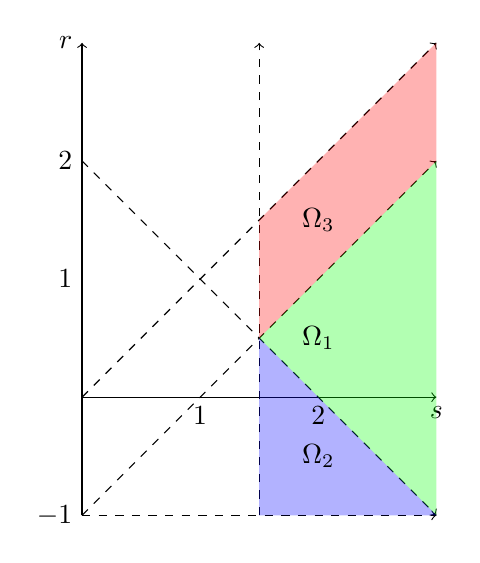
\begin{tikzpicture}[scale=1.5]
% Draw thin grid lines with color 40% gray + 60% white
% Draw x and y axis lines
\draw [->] (0,0) -- (3,0) node [below] {$s$};
\draw [->] (0,-1) -- (0,3) node [left] {$r$};
\draw [->, dashed] (0,0) -- (3,3);
\draw [->, dashed] (0,-1) -- (3,2);
\draw [->, dashed] (0,2) -- (3,-1);
\draw [->, dashed] (0,-1) -- (3,-1);
\draw [->, dashed] (3/2,-1) -- (3/2, 3);
\fill[color=green, fill opacity=0.3] (1.5, 0.5) -- (3,2) -- (3,0) -- (3,-1);
\fill[color=red, fill opacity=0.3] (1.5, 0.5) -- (1.5,1.5) -- (3,3) -- (3,2);
\fill[color=blue, fill opacity=0.3] (1.5, 0.5) -- (1.5, -1) -- (3, -1);
\foreach \x/\xtext in {1, 2}
\draw[shift={(\x,0)}]  node[below] {$\xtext$};
\foreach \y/\ytext in {-1, 1, 2}
\draw[shift={(0,\y)}]  node[left] {$\ytext$};
\draw (2,1.5) node {$\Omega_{3}$};
\draw (2,0.5) node {$\Omega_{1}$};
\draw (2,-0.5) node {$\Omega_{2}$};
\end{tikzpicture}
\end{center}
%
%
Then for two initial data $u_{0}, v_{0} \in B_{H^{s}}(R)$, there exist unique
corresponding solutions \\ $u(x,t), v(x,t)$ for $0 \le t \le T= T(R)$ to the
HR equation \eqref{hyperelastic-rod-equation} which satisfy 
%
%
\begin{equation*}
\begin{split}
\| u(t) - v(t) \|_{H^{r}} \le C \| u_{0} - v_{0} \|_{H^{r}}^{\alpha(s, r)},
\quad 0
\le t \le T
\end{split}
\end{equation*}
%
%
where 
%
%
\begin{equation*}
\begin{split}
\alpha = 
\begin{cases}
1, \quad & (s,r) \in \Omega_{1} 
\\
2(s-1)/(s-r),  \quad & (s, r) \in \Omega_{2}
\\
s-r, \quad & (s, r) \in \Omega_{3}.
\end{cases}
\end{split}
\end{equation*}
%
%
%%%%%%%%%%%%%%%%%%%%%%%%%%%%%%%%%%%%%%%%%%%%%%%%%%%%%
%
%
%                Main theorem
%
%
%%%%%%%%%%%%%%%%%%%%%%%%%%%%%%%%%%%%%%%%%%%%%%%%%%%%%
%
%
We remark that this result is sharper then the analogue obtained in
\cite{Chen:2011fk} for the $b$-family. We are confident that the techniques
applied here can be applied to sharpen the results obtained in
\cite{Chen:2011fk}.

The document is structured as follows. We first prove 
\cref{thm:hr-non-unif-dependence} on the line and 
then on the circle.
As mentioned above, we begin with two sequences of
appropriate approximate solutions and then 
we construct  actual solutions
coinciding at time zero  with the approximate solutions.
The key step is to show that  the $H^s$-size of
the difference between approximate and actual solutions 
converges to zero (see \cref{applelem:bound_for_difference-of-approx-and-actual-soln}
and \cref{prop:bound_for_difference-of-approx-actual-soln}). 
We then prove \cref{thm:HR_existence_continuous_dependence} 
using a Galerkin-type argument and energy estimates. Using the tools (energy estimates, commutator estimate, and multiplier estimate) used to prove \cref{thm:HR_existence_continuous_dependence}, we will then prove \cref{thm:main-thm}. 
%
%
%	
%
%
%
%
%%%%%%%%%%%%%%%%%%%%%%%%
%
%           Proof of  \cref on the line
%
%%%%%%%%%%%%%%%%%%%%%%%%
%
%
%
%
%
\section{Proof of Non-Uniform Dependence on the Line}
\label{sec:2}
%
%
%
%
We begin by outlining the method of the proof,
as it has been applied for the case $\gamma=1$ in \cite{Himonas:2009fk}.
We will show  that there there exist two sequences of solutions 
$u_n(t)$
and $v_n(t)$ in $C([-T, T], H^s)$ such that
%
%
%
%
\begin{equation}
\label{h-s-bdd}
\| u_n(t)  \|_{H^s}
+
\| v_n(t)  \|_{H^s}
\lesssim
1,
\end{equation}
%
%
%
%
%
\begin{equation}
\label{zero-limit-at-0}
\lim_{n\to\infty}
\|
u_n(0)
-
v_n(0)
\|_{H^s}
=
0,
\end{equation}
%
%
%
%
and
%
%
%
%
\begin{equation}
\label{bdd-away-from-0}
\liminf_{n\to\infty}
\|
u_n(t)
-
v_n(t)
\|_{H^s}
\gtrsim
|\sin ( \gamma t)|,
\quad
| \gamma t|\le 1.
\end{equation}%
%
%
We accomplish this in two steps.
First, we will construct two sequences of approximate solutions
satisfying the above properties.
Then, we will construct two sequences of actual solutions 
coinciding with the approximate solutions at time zero.
The key point of this method is that 
the difference between solutions and approximate solutions
decays rapidly.

%
%
For this method, it is more convenient 
to rewrite the Cauchy problem for the HR equation 
in the following non-local form
%
%
\begin{align}
& \p_t u =  -\gamma u \p_x u -
\Lambda^{-1} \left[ \frac{3-\gamma}{2}u^2 +
\frac{\gamma}{2} \left( \p_x u \right)^2
\right],
\label{apple1'}
\\
&  u(x,0) = u_0(x), \; \; x \in \rr, \; \; t \in \rr
\label{apple2'}
\end{align}
%
%
where 
\begin{equation*}
\Lambda^{-1} = \p_x (1 - \p_x^2)^{-1}.
\end{equation*}
%
%
%
%
%
%

\subsection{Approximate solutions}
Following \cite{Himonas:2009fk}, our approximate solutions
\\ $u^{\omega, \lambda} = u^{\omega,
\lambda}(x,t)$ to \eqref{apple1'}-\eqref{apple2'} will
consist of a low frequency and a high frequency part,
i.e.
%
%
%
%
\begin{equation}
\label{apple1}
u^{\omega,\lambda} = u_\ell + u^h
\end{equation}
%
%
%
%
where $\omega$ is in a bounded set of $\rr$ and $\lambda > 0$. The high frequency part is given by 
%
%
%
%
\begin{equation}
\begin{split}
u^h = u^{h,\omega,\lambda}(x,t) =
\lambda^{-\frac{\delta}{2} -s}
\phi \left (\frac{x}{\lambda^\delta}\right )
\cos(\lambda x - \gamma \omega t)
\end{split}
\end{equation}
%
%
%
%
where $\phi$ is a $C^\infty$ cut-off function such that
%
%
%
%
\begin{equation*}
\phi = \begin{cases}
1, &\text{if $|x|<1$,} \\
0, &\text{if $|x| \ge 2,$} \end{cases}
\end{equation*}
%
%
%
%
and by \cref{thm:HR_existence_continuous_dependence} 
we let the low frequency part $u_\ell = u_{l,
\omega, \lambda}(x,t)$ be the unique solution to the Cauchy problem
%
%
\begin{align}
\label{u-l-apple1'}
& \p_t u_\ell = -\gamma u_\ell \p_x u_\ell -
\Lambda^{-1} \left[ \frac{3-\gamma}{2}(u_\ell)^2 +
\frac{\gamma}{2} \left( \p_x u_\ell \right)^2
\right],
\\
& u_\ell(x,0) = \omega \lambda^{-1} \tilde{\phi} \left(
\frac{x}{\lambda^{\delta}}
\right), \quad x \in \rr, \quad t \in \rr
\label{apple1ah}
\end{align}
%
%
%
%
where $\tilde{\phi}$ is a $C^{\infty}_0(\rr)$ function such that
%
%
%
%
\begin{equation}
\label{apple1ah7}
\tilde{\phi}(x) = 1 \; \;  \text{if} \; \;
x \in \text{supp} \; \phi.
\end{equation}
%
%
%
%
We remark that for $\lambda >>1$ and $\delta < 2$ the approximate solutions 
$u^{\omega, \lambda}$ share a common lifespan $T >> 1$. To see why, we 
first note that the high frequency part $u^{h, \omega, \lambda}$ has 
infinite lifespan by the following, whose 
proof can be found in \cite{Himonas:2009fk}: 
%
%
\begin{lemma}
\label{applea}
Let $\psi \in S(\rr)$, $\alpha \in \rr$. Then for $s \ge 0$ we have
%
%
\begin{equation}
\begin{split}
\lim_{\lambda \to \infty} \lambda^{-\frac{\delta}{2}-s}
\|\psi \left( \frac{x}{\lambda^\delta} \right)\cos(\lambda
x - \alpha) \|_{H^s(\rr)} = \frac{1}{\sqrt
2}\|\psi\|_{L^2(\rr)}.
\label{apple6}
\end{split}
\end{equation}
%
%
Relation \eqref{apple6} remains true if $\cos$ is
replaced by $\sin$.
\end{lemma}
%
%
For the low frequency part $u_{\ell, \omega, \lambda}$, we apply \eqref{Life-span-est} and the estimate
%
%
\begin{equation}
\begin{split}
\label{tildphi}
\|\tilde{\phi}\left( \frac{x}{\lambda^\delta}
\right)\|_{H^{k}(\rr)} \le
\lambda^{\frac{\delta}{2}}\|\tilde{\phi}\|_{H^{k}(\rr)},
\quad k\ge 0
\end{split}
\end{equation}
%
%
to obtain a lower bound for its lifespan
%
\begin{equation*}
\label{lifespan-bound-1}
\begin{split}
T_{\ell, \omega,\lambda} \ge \frac{1}{2 c_s \|u_{\ell, \omega, \lambda}(0)\|_{H^s(\rr)}} = 
\frac{1}{2 c_s |\omega|
\lambda^{\frac{\delta}{2}-1}\|\tilde{\phi}\|_{H^s(\rr)}} >> 1.
\end{split}
\end{equation*}
%
%
Since $\omega$ belongs to a bounded subset of $\rr$, the existence of a 
common lifespan $T >> 1$ follows. 
%
%

Substituting the
approximate solution $u^{\omega, \lambda} = u_\ell + u^h$ into the HR
equation, we see that the error
$E$ of our approximate solution is given by
%
%
\begin{equation*}
E=E_1 + E_2 + \dots + E_8
\end{equation*}
%
%
where
%
%
\begin{equation}
\label{all_errors_together}
\begin{split}
E_1 & = \gamma \lambda^{1 -\frac{\delta}{2}-s}  \left[ u_\ell(x,0) - u_\ell(x,t)
\right] \phi\left(
\frac{x}{\lambda^ \delta}
\right)\sin(\lambda x - \gamma \omega t),
\\
E_2 & = \gamma \lambda^{-\frac{3\delta}{2}-s}
u_\ell(x,t) \cdot \phi'\left( \frac{x}{\lambda^\delta} \right)\cos\left( \lambda
x - \gamma \omega t
\right),
\\
E_3 & = \gamma u^h \p_x u_\ell, \; \; E_4 = \gamma u^h \p_x u^h, \ E_5  = 
\frac{3-\gamma}{2} \Lambda^{-1} \left[  \left( u^h \right)^2 \right], \\
E_6 & = (3- \gamma)\Lambda^{-1}
\left[ u_\ell u^h \right], \  E_7 = \frac{\gamma}{2} \Lambda^{-1} \left[ 
\left(
\p_x u^h \right)^2 \right ], \ E_8 = \gamma \Lambda^{-1} \left[  \p_x u_\ell \p_x u^h \right].
\end{split}
\end{equation}
%
%
%
Next we prove the decay of the error:
%
%
\begin{proposition}
Let $1<\delta<2$. Then for $s > 1$, bounded $\omega$, and
$\lambda >>1$ we are assured the decay of the error $E$ of the
approximate solutions to the HR equation. Specifically
%
%
%
\begin{equation}
\label{E-est}
\|E(t)\|_{H^1(\rr)} \lesssim \lambda^{\frac{\delta}{2} -s}, \quad |t| \le 
T.
\end{equation}
%
%
%
\end{proposition}
%
%
%
\begin{proof}
    It will suffice to estimate the $H^1$ norms of each $E_i$. \vspace{0.25cm}\\
{\bf Estimating the $H^1$ norm of $\hyperref[all_errors_together]{E_1}$.} 
We have
%
%
\begin{equation}
\label{fw-est}
\begin{split}
\|E_1\|_{H^1(\rr)}
& = \| \gamma \lambda^{1 -\frac{\delta}{2}-s} \left[ u_\ell(x,0) - u_\ell(x,t) \right]
\phi\left( \frac{x}{\lambda^\delta}
\right ) \sin (\lambda x - \gamma \omega t )\|_{H^1(\rr)}
\\
& \lesssim \lambda^{1 -\frac{\delta}{2} -s } \|\left[ u_\ell(x,0) - 
u_\ell(x,t)
\right] \phi\left( \frac{x}{\lambda^\delta} \right )
\sin\left( \lambda x - \gamma \omega t
\right) \|_{H^1(\rr)}.
\end{split}
\end{equation}
%
%
Applying the inequality 
%
%
\begin{equation*}
\label{applec}
\|fg\|_{H^1(\rr)} \lesssim \|f\|_{C^1(\rr)} \|g\|_{H^1(\rr)}
\end{equation*}
%
%
%
%
%
%
%
%
to estimate \eqref{fw-est} gives
%
%
\begin{equation}
\begin{split}
\|E_1\|_{H^1(\rr)} \lesssim \lambda^{1 - \frac{\delta}{2} -s } \|\phi
\left( \frac{x}{\lambda^\delta} \right) \sin (\lambda x - \gamma \omega t)
\|_{C^1(\rr)} \|[u_\ell (x,0) - u_\ell (x,t) ] \|_{H^1(\rr)}.
\label{apple14}
\end{split}
\end{equation}
%
%
We now estimate the right-hand side of \eqref{apple14} in pieces. First, 
note that routine computations give
%
%
\begin{equation}
\begin{split}
\|\phi\left( \frac{x}{\lambda^\delta} \right) \sin(\lambda x - \gamma 
\omega t)
\|_{C^1(\rr)}
\lesssim \lambda.
\label{apple15}
\end{split}
\end{equation}
%
%
Next, we observe that the fundamental 
theorem
of calculus and Minkowski's inequality give
%
%
%
%
\begin{equation}
\begin{split}
\|u_\ell(x,t) - u_\ell(x,0)\|_{H^1(\rr)}
& =  \| \int_0^t \p_\tau
u_\ell(x,\tau) \; d \tau \|_{H^1(\rr)}
\le \int_0^t \|\p_\tau u_\ell (x,\tau) \|_{H^1(\rr)} \; d \tau.
\label{apple100}
\end{split}
\end{equation}
%
%
We want to estimate the right-hand side of \eqref{apple100}. Recalling
\eqref{apple1'}, we have
%
%
\begin{equation}
\label{apple101}
\begin{split}
\|\p_\tau u_\ell(x,\tau) \|_{H^1(\rr)}
& \le \|\gamma u_\ell \p_x u_\ell \|_{H^1(\rr)}
+ \|\Lambda^{-1} \left[
\frac{3-\gamma}{2} (u_\ell)^2 + \frac{\gamma}{2} \left( \p_x u_\ell 
\right)^2
\right] \|_{H^1(\rr)}.
\end{split}
\end{equation}
%
%
Applying the algebra property of Sobolev spaces, we obtain
%
%
\begin{equation*}
\begin{split}
\|\gamma u_\ell \p_x u_\ell \|_{H^1(\rr)} &
\lesssim \|u_\ell\|_{H^2(\rr)}^2
\end{split}
\end{equation*}
%
%
which yields 
%
%
\begin{equation}
\begin{split}
\|\gamma u_\ell \p_x u_\ell \|_{H^1(\rr)} \lesssim \lambda^{-2 + \delta}
\label{apple102}
\end{split}
\end{equation}
%
%
%
%
by the following:
%
%
%
%%%%%%%%%%%%%%%%%%%%%%%%%%%%%%%%%%%%%%%%%%%%%%%%%%%%%
%
%
% 				
%
%
%%%%%%%%%%%%%%%%%%%%%%%%%%%%%%%%%%%%%%%%%%%%%%%%%%%%%
%
%
%
\begin{lemma}
\label{appleb}
Let $0<\delta<2$, $\lambda >>1$, with $\omega$ belonging to a bounded
subset of $\rr$. Then the initial value problem
\eqref{u-l-apple1'}-\eqref{apple1ah}
has a unique solution
$u_\ell \in C( [-T,T], H^s(\rr))$ for all $s
> 3/2$ which satisfies
%
%
\begin{equation}
\label{apple10'}
\|u_\ell(t)\|_{H^s(\rr)} \le c_s \lambda^{-1 +
\frac{\delta}{2}}, \quad |t| \le T.
\end{equation}
%
%
\end{lemma}
%
An analogous result can be found in \cite{Himonas:2009fk}. 
%
%
%
Applying the inequality 
%
\begin{equation*}
\begin{split}
\|\Lambda^{-1} f \|_{H^1(\rr)} \le \|f\|_{L^2(\rr)},
\label{apple27}
\end{split}
\end{equation*}
%
%
and the algebra property of Sobolev spaces, we obtain
%
%
\begin{equation*}
\begin{split}
\|\Lambda^{-1} \left[ \frac{3-\gamma}{2}(u_\ell)^2 +
\frac{\gamma}{2}\left( \p_x u_\ell \right)^2 \right] \|_{H^1(\rr)}
& \lesssim \|u_\ell\|_{H^2(\rr)}^2
\end{split}
\end{equation*}
%
%
which by \cref{appleb} gives
%
%
\begin{equation}
\begin{split}
\|\Lambda^{-1} \left[ \frac{3-\gamma}{2}(u_\ell)^2 +
\frac{\gamma}{2}\left( \p_x u_\ell \right)^2 \right] \|_{H^1(\rr)}
\lesssim \lambda^{-2 + \delta}, \quad |t| \le T.
\label{apple104}
\end{split}
\end{equation}
%
%
Substituting \eqref{apple102} and \eqref{apple104} into the right-hand side 
of
\eqref{apple101}, and recalling \eqref{apple100}, we obtain
%
%
\begin{equation}
\begin{split}
\|u_\ell(x,t) - u_\ell(x,0)\|_{H^1(\rr)} \lesssim \lambda^{-2 + \delta}, 
\quad |t| \le T.
\label{apple1055}
\end{split}
\end{equation}
%
Substituting \eqref{apple1055} and \eqref{apple15} into \eqref{apple14}, we obtain
%
%
\begin{equation}
  \label{apple105}
\begin{split}
  \| E_{1} \|_{H^{1}} \lesssim \lambda^{\delta/2 -s}.
\end{split}
\end{equation}
%
%

{\bf Estimating the $H^1$ norm of $\hyperref[all_errors_together]{E_2}$.} Applying  \eqref{applec}, we have
\begin{equation}
	\begin{split}
		\|E_2\|_{H^1(\rr)} 
		& = \gamma \lambda^{-\frac{3 \delta}{2} -s } \|u_\ell(x,t) \cdot
		\phi'\left( \frac{x}{\lambda^\delta} \right) \cos (\lambda x - \gamma \omega t)
		\|_{H^1(\rr)}
		\\
		& \lesssim_{s} \gamma \lambda^{\frac{-3 \delta}{2} -s } \|u_\ell(x,t) \|_{H^1(\rr)}
		\|\phi'\left( \frac{x}{\lambda^\delta} \right )
		\cos(\lambda x - \gamma \omega t 
		\|_{C^1(\rr)}.
		\label{apple18} 
	\end{split}
\end{equation}
We note that
\begin{equation*}
	\begin{split}
		& \|\phi'\left( \frac{x}{\lambda^\delta} \right) \cos(\lambda x - \gamma \omega t)
		\|_{C^1(\rr)}
		\\
		& \le \|\phi' \left( \frac{x}{\lambda^\delta} \right)\|_{L^\infty(\rr)} +
		\lambda \|\phi'\left( \frac{x}{\lambda^\delta} \right)\|_{L^\infty(\rr)}
		+ \lambda^{-\delta} \|\phi''\left( \frac{x}{\lambda^\delta} \right)
		\|_{L^\infty(\rr)}
	\end{split}
\end{equation*}
which gives
\begin{equation}
	\begin{split}
		\|\phi'\left( \frac{x}{\lambda^\delta} \right) \cos(\lambda x - \gamma \omega t)
		\|_{C^1(\rr)} \lesssim \lambda.
		\label{apple19}
	\end{split}
\end{equation}
Applying estimates \eqref{apple19} and \eqref{apple10'} to \eqref{apple18}, we obtain
\begin{equation*}
	\begin{split}
	\label{apple20}
	\|E_2\|_{H^1(\rr)} \lesssim \lambda^{-\delta -s }.
\end{split}
\end{equation*}
%
%
%
%
{\bf Estimating the $H^1$ norm of $\hyperref[all_errors_together]{E_3}$.} 
By  \eqref{applec}, we deduce
\begin{equation}
	\begin{split}
		\|\gamma u^h \p_x u_\ell \| \lesssim \|u^h\|_{C^1(\rr)}
		\|u_\ell\|_{H^1(\rr)}.
		\label{apple21}
	\end{split}
\end{equation}
Now, note that
\begin{equation}
	\begin{split}
		\|u^h\|_{L^\infty(\rr)} 
		& = \lambda^{-\frac{\delta}{2} -s } \|\phi\left( \frac{x}{\lambda^\delta}
		\right) \cos \left( \lambda x - \gamma \omega t \right) \|_{L^\infty(\rr)}
		\\
		& \lesssim \lambda^{-\frac{\delta}{2} -s }
		\label{apple22}
	\end{split}
\end{equation}
and 
\begin{equation}
	\begin{split}
		& \|\p_x u^h \|_{L^\infty(\rr)}
		\\
		& = \lambda^{-\frac{\delta}{2}-s} \|\phi\left(
		\frac{x}{\lambda^\delta}
		\right) \cdot -\lambda \sin(\lambda x - \gamma \omega t) + \lambda^{-\delta}
		\phi'\left( \frac{x}{\lambda^\delta}\right) \cos(\lambda x - \gamma \omega
		t) \|_{L^\infty(\rr)}
		\\
		& \lesssim \lambda^{1 - \frac{\delta}{2} -s }.
		\label{apple23}
	\end{split}
\end{equation}
Therefore, from \eqref{apple22} and \eqref{apple23} it follows that
\begin{equation}
	\begin{split}
		\|u^h\|_{C^1(\rr)} \lesssim \lambda^{-\frac{\delta}{2} -s } + \lambda^{1
		-\frac{\delta}{2} -s}
		\approx \lambda^{1- \frac{\delta}{2} -s}.
		\label{apple24}
	\end{split}
\end{equation}
Substituting estimates \eqref{apple24} and  \eqref{apple10'} into \eqref{apple21} we obtain
\begin{equation}
	\begin{split}
		\|\gamma u^h \p_x u_\ell \|_{H^1(\rr)} \lesssim \lambda^{-s}.
		\label{apple24'}
	\end{split}
\end{equation}
%
{\bf Estimating the $H^1$ norm of $\hyperref[all_errors_together]{E_4}$.} Applying  \eqref{applec} we have
\begin{equation}
	\begin{split}
		\|\gamma u^h \p_x u^h\|_{H^1(\rr)} \lesssim \|u^h\|_{C^1(\rr)}
		\|u^h\|_{H^1(\rr)}.
		\label{apple25}
	\end{split}
\end{equation}
Substituting in \eqref{apple24}, and observing that $\|u^h\|_{H^1(\rr)} \lesssim 1$ for $\lambda >>1$ by 
\cref{applea}, we obtain
\begin{equation}
	\begin{split}
		\|u^h \p_x u^h \|_{H^1(\rr)} \lesssim \lambda^{1-\frac{\delta}{2}-s}.
		\label{apple26}
	\end{split}
\end{equation}
%
%
%
{\bf Estimating the $H^1$ norm of $\hyperref[all_errors_together]{E_5}$.}
Applying \eqref{apple27}, we obtain
\begin{equation}
	\begin{split}
		\|E_5\|_{H^1(\rr)}
		& = \|\Lambda^{-1}\left[ \frac{3-\gamma}{2}(u^h)^2
		\right]\|_{H^1(\rr)}
		\\
		& \lesssim \|u^h\|_{L^\infty(\rr)} \|u^h\|_{L^2(\rr)}.
		\label{apple28}
	\end{split}
\end{equation}
Substituting \eqref{apple6} and \eqref{apple22} into \eqref{apple28}, we conclude that
\begin{equation}
	\begin{split}
		\|E_5\|_{H^1(\rr)} \lesssim \lambda^{-\frac{\delta}{2}-s}.
		\label{apple29}
	\end{split}
\end{equation}
%
%
%
%
%
{\bf Estimating the $H^1$ norm of $\hyperref[all_errors_together]{E_6}$.} Applying \eqref{apple27}, we obtain
\begin{equation}
	\begin{split}
		\|E_6\|_{H^1(\rr)} 
		& = \|\Lambda^{-1} \left[ (3 -\gamma) u_\ell u^h \right]\|_{H^1(\rr)}
		\\
		& \lesssim \|u_\ell\|_{L^2(\rr)} \|u^h\|_{L^\infty(\rr)}
		\label{apple30}
	\end{split}
\end{equation}
which by  \cref{appleb} and \eqref{apple22} reduces to
\begin{equation}
	\begin{split}
		\|E_6\|_{H^1(\rr)} \lesssim \lambda^{-1-s}.
		\label{apple31}
	\end{split}
\end{equation}
%
%
%
%
%
{\bf Estimating the $H^1$ norm of $\hyperref[all_errors_together]{E_7}$.} Applying \eqref{apple27}, we obtain
\begin{equation}
	\begin{split}
		\|E_7\|_{H^1(\rr)} 
		& = \|\Lambda^{-1} \left[ \frac{\gamma}{2}\left( \p_x u \right)^2
		\right]\|_{H^1(\rr)}
		\\
		& \lesssim  \|\p_x u^h\|_{L^\infty(\rr)} \|u^h\|_{H^1(\rr)}.
		\label{apple32}
	\end{split}
\end{equation}
which by  \cref{applea} and \eqref{apple23} reduces to
\begin{equation}
	\begin{split}
		\|E_7\|_{H^1(\rr)} \lesssim \lambda^{1-\frac{\delta}{2}-s}.
		\label{apple33'}
	\end{split}
\end{equation}
%
%
%
%
%
{\bf Estimating the $H^1$ norm of $\hyperref[all_errors_together]{E_8}$.} Applying \eqref{apple27}, we have
\begin{equation}
	\begin{split}
		\|E_8\|_{H^1(\rr)}
		& = \|\Lambda^{-1}\left[ \gamma \p_x u_\ell \p_x u^h \right]\|_{H^1(\rr)}
		\\
		& \lesssim \|u_\ell\|_{H^2(\rr)} \|\p_x u^h\|_{L^\infty(\rr)}
		\label{apple33}
	\end{split}
\end{equation}
which by  \cref{appleb} and \eqref{apple23} reduces to
\begin{equation}
	\begin{split}
		\|E_8\|_{H^1(\rr)} \lesssim \lambda^{-s}.
		\label{apple34}
	\end{split}
\end{equation}
Collecting all our estimates for the $E_i$ and recalling that we have assumed
$1<\delta<2$, we obtain
\begin{equation*}
	\begin{split}
		\|E\|_{H^1(\rr)}
		 \lesssim \lambda^{\frac{\delta}{2} -s }, \qquad \lambda >>1
	\end{split}
\end{equation*}
which completes the proof.
\end{proof}
%
%
%
%
%
\subsection{Construction of solutions}
We wish now to estimate the difference between approximate and actual 
solutions to
the HR i.v.p.\ with common initial data. Let
$u_{\omega,\lambda}(x,t)$ be the unique solution to the HR equation
with initial data $u^{\omega,\lambda}(x,0)$. That is,
$u_{\omega,\lambda}$ solves the initial value problem
\begin{align}
& \p_t u_{\omega,\lambda} = - \gamma u_{\omega,\lambda} \p_x 
u_{\omega,\lambda} - \Lambda^{-1} \left[
\frac{3- \gamma}{2}\left( u_{\omega,\lambda} \right)^2 + 
\frac{\gamma}{2}\left(
\p_x u_{\omega,\lambda} \right)^2
\right], \label{apple50}
\\
& u_{\omega,\lambda}(x, 0) = u^{\omega,\lambda}(x,0) = \omega \lambda^{-1}
\tilde{\phi} \left( \frac{x}{\lambda^\delta} \right)
+ \lambda^{-\frac{\delta}{2} -s}
\phi\left( \frac{x}{\lambda^\delta} \right) \cos(\lambda x).
\label{apple41}
\end{align}
%
%
%
We will now prove that the $H^1(\rr)$ norm of the difference decays: 
%
%%%%%%%%%%%%%%%%%%%%%%%%%%%%%%%%%%
%
%
%
%
%
%    : H^1 bound_for_difference-of-approx-and-actual-soln
%
%
%
%
%
%
%%%%%%%%%%%%%%%%%%%%%%%%%%%%%%%%%
%
%
%
\begin{proposition}
\label{applelem:bound_for_difference-of-approx-and-actual-soln}
%
Let $v = u^{\omega,\lambda} - u_{\omega,\lambda}$, with $\lambda >>1$.
Then, for $s > 1$ and $1<\delta<2$ we have
%
%
\begin{equation} \|
v(t)
\|_{H^1(\rr)}
\lesssim \lambda^{\frac{\delta}{2} -s}, \quad
|t| \le T.
\end{equation}
%
%
\end{proposition}
%
%
\begin{proof} First we observe that $v$ satisfies 
%
%
\begin{equation*}
\begin{split}
\p_t v & = E + \gamma(v \p_x v - v \p_x u^{\omega,\lambda} - 
u^{\omega,\lambda} \p_x v) \\
& + \Lambda^{-1}  \left[ \frac{3-
\gamma}{2}v^2 + \frac{\gamma}{2}\left( \p_x v \right)^2 - \left(
3 - \gamma \right)u^{\omega,\lambda} v -
\gamma \p_x u^{\omega,\lambda} \p_x v \right].
\end{split}
\end{equation*}
%%
It follows immediately that
\begin{equation}
\label{applev-dtv-pseudo-functional-equalityu}
\begin{split}
v(1-\p_x^2)\p_t v &= v(1- \p_x^2)E + v\gamma(1- \p_x^2)(v\p_x v 
- v\p_x u^{\omega,\lambda} -
u^{\omega,\lambda} \p_x v)
\\
&+ v\p_x \left[ \frac{3-\gamma}{2}v^2 + \frac{\gamma}{2}(\p_x v)^2 -
(3-\gamma)u^{\omega,\lambda} v - \gamma \p_x u^{\omega,\lambda} \p_x v \right].
\end{split}
\end{equation}
Applying the relation $v\p_t v = v(1-\p_x^2) \p_t v + v\p_x^2 \p_t v$ to
\eqref{applev-dtv-pseudo-functional-equalityu}, we obtain
\begin{equation}
\label{pre-int}
\begin{split}
v \p_t v &= v(1- \p_x^2)E + v\gamma(1- \p_x^2)(v\p_x v - v\p_x u^{\omega,\lambda} -
u^{\omega,\lambda} \p_x v)
\\
&+ v\p_x \left[ \frac{3-\gamma}{2}v^2 + \frac{\gamma}{2}(\p_x v)^2 -
(3-\gamma)u^{\omega,\lambda} v - \gamma \p_x u^{\omega,\lambda} \p_x v
\right] + v\p_x^2 \p_t v.
\end{split}
\end{equation}
Adding $\p_x v \p_t \p_x v$ to both sides of \eqref{pre-int} and 
integrating gives
\begin{equation}
\label{appleenergy-estu}
\begin{split}
&\frac{1}{2} \frac{d}{dt} \|v\|_{H^1(\rr)}^2  
\\
& =  \int_{\rr} v(1-\p_x^2)E dx
\\
& - \gamma \int_{\rr}  v(1-\p_x^2)(v\p_x u^{\omega,\lambda} + u^{\omega,\lambda} \p_x v) dx
\\
&- \int_{\rr}\left[ \left( 3-\gamma \right)v \p_x\left( u^{\omega,\lambda}v \right) + \gamma v
\p_x \left( \p_x u^{\omega,\lambda} \p_x v \right)\right]dx
\\
&+  \int_{\rr}
\left[ \gamma v \left( 1-\p_x^2 \right)\left( v \p_x v \right) + v
\p_x \left( \frac{3-\gamma}{2} v^2 + \frac{\gamma}{2}\left( \p_x v \right)^2
\right) \right . +  v \p_x^2 \p_t v + \p_x v \p_t \p_x v\bigg]dx.
\end{split}
\end{equation}
Noting that the last integral can be rewritten as 
\begin{equation*}
\begin{split}
\int_{\rr} \left[ \p_x (v^3) - \gamma \p_x (v^2 \p_x^2 v) + \p_x\left( v \p_t
\p_x v
\right) \right]dx  = 0
\end{split}
\end{equation*}
%
we can simplify \eqref{appleenergy-estu} to obtain
%
%
\begin{equation}
\label{appleenergy-est}
\begin{split}
\frac{1}{2} \frac{d}{dt} \|v\|_{H^1(\rr)}^2  
& = 
\int_{\rr}  v(1-\p_x^2)E dx\\
&-
\gamma \int_{\rr} v(1-\p_x^2)(v\p_x u^{\omega,\lambda} + 
u^{\omega,\lambda} \p_x v) dx
\\
&- \int_{\rr}\left[ \left( 3-\gamma \right)v \p_x\left( u^{\omega,\lambda}v 
\right) + \gamma v
\p_x \left( \p_x u^{\omega,\lambda} \p_x v \right)\right]dx.
\end{split}
\end{equation}
%
%
We now estimate the three integrals in the right-hand side of 
\eqref{appleenergy-est}. Integrating by parts and applying Cauchy-Schwartz,  
we obtain
%
%
%
\begin{equation}
\begin{split}
\label{applefirst_piece}
& \left |\int_{\rr} \left [v (1- \p_x^2)E \right ] dx \right |
\lesssim
\|v\|_{H^1(\rr)} \|E\|_{H^1(\rr)}
\end{split}
\end{equation}
for the first integral. Applying Parseval and H\"older gives
%
%
\begin{equation}
\begin{split}
\label{applesecond-piece-final}
& \left | -\gamma \int_{\rr}
\left[ v\left( 1-\p_x^2 \right)\left( v \p_x u^{\omega,\lambda} + 
u^{\omega,\lambda} \p_x v
\right) \right] dx \right |
\\
& \lesssim \left( \|u^{\omega,\lambda}\|_{L^\infty(\rr)}\| + \|\p_x 
u^{\omega,\lambda}
\|_{L^\infty(\rr)} \right .  + \|\p_x^2 u^{\omega,\lambda} 
\|_{L^\infty(\rr)}
\big )\|v\|_{H^1(\rr)}^2
\end{split}
\end{equation}
for the second integral, and applying H\"older gives 
\begin{equation}
\begin{split}
\label{applelast_piece_final}
& \left | -\int_{\rr} \left[ \left( 3-\gamma \right)v
\p_x \left( u^{\omega,\lambda} v \right) + \gamma
v \p_x \left( \p_x u^{\omega,\lambda} \p_x v \right)\right]dx \right |
\\
& \lesssim \big(
\|u^{\omega,\lambda}\|_{L^\infty(\rr)}
+ \|\p_x u^{\omega,\lambda} \|_{L^\infty(\rr)} \big)
\|v\|_{H^1(\rr)}^2
\end{split}
\end{equation}
%
%
%
for the third integral. Combining 
\eqref{applefirst_piece}-\eqref{applelast_piece_final}, we 
obtain
%
%
\begin{equation}
\begin{split}
\label{appleenergy-estimate-best}
\frac{d}{dt} \|v(t)\|_{H^1(\rr)}^2
& \lesssim \left( \|u^{\omega,\lambda}\|_{L^\infty(\rr)} + \|
\p_x u^{\omega,\lambda} \|_{L^\infty(\rr)} + \|\p_x^2 u^{\omega,\lambda} 
\|_{L^\infty (\rr)} \right)
\|v\|_{H^1(\rr)}^2 \\
&+ \|v\|_{H^1(\rr)} \|E\|_{H^1(\rr)}.
\end{split}
\end{equation}
%
%
Assume $\lambda >>1$. A straightforward calculation of derivatives yields
%
%
\begin{equation*}
\begin{split}
\|u^h\|_{L^\infty(\rr)} + \|\p_x u^h\|_{L^\infty(\rr)} + \|\p_x^2
u^h\|_{L^\infty(\rr)} \lesssim \lambda^{- \frac{\delta}{2} - s +2 }.
\label{apple53}
\end{split}
\end{equation*}
%
%
Furthermore, by the Sobolev Imbedding Theorem and \cref{appleb}, we have
%
%
%
%
\begin{equation*}
\begin{split}
\|u_\ell\|_{L^\infty(\rr)} + \|\p_x u_\ell \|_{L^\infty(\rr)} + \|\p_x^2
u_\ell\|_{L^\infty(\rr)}
& \le c_s \|u_\ell\|_{H^3(\rr)} 
\lesssim \lambda^{-1 + \frac{\delta}{2}}, 
\quad |t| \le T.
\label{apple55}
\end{split}
\end{equation*}
%
%
Hence
%
%
\begin{equation}
\begin{split}
\|u^{\omega,\lambda}\|_{L^\infty(\rr)} + \|\p_x 
u^{\omega,\lambda}\|_{L^\infty(\rr)} + \|\p_x^2
u^{\omega,\lambda}\|_{L^\infty(\rr)}
& \lesssim \lambda^{-\rho_s}, \quad |t| \le T
\label{apple56}
\end{split}
\end{equation}
%
%
where $\rho_s = \text{min} \Big\{ \frac{\delta}{2} + s -2, \; 1-
\frac{\delta}{2} \Big\}$.  Note that for $s>1$, we can assure $\rho_s > 0$
by choosing a suitable $1<\delta<2$.
Substituting \eqref{E-est} and \eqref{apple56} into \eqref{appleenergy-estimate-best},
we get
%
%
\begin{equation}
\label{apple58}
\frac{d}{dt} \|v(t)\|_{H(\rr)}^2 \lesssim \lambda^{-\rho_s}
\|v\|_{H^1(\rr)}^2 + \lambda^{-r_s}
\|v \|_{H^1(\rr)}, \quad |t| \le T.
\end{equation}
%
%
Applying Gronwall's inequality completes the proof. 
\end{proof}
%
%
%
%

\subsection{Non-Uniform Dependence for $s>3/2$}
Let $u_{\pm 1,\lambda}$ be solutions to the HR i.v.p.\ with initial 
data $u^{\pm 1,
n}(0)$. We wish to show that the $H^s$ norm of the difference of $u_{\pm 1,
n}$ and the associated approximate solution $u^{\pm 1,\lambda}$
decays as $\lambda \to \infty$. Note that
%
%
\begin{equation*}
\begin{split}
\label{apple62}
\|u^{\pm 1, \lambda}(t)\|_{H^{2s-1}(\rr)}
& \le \|u_{\ell, \pm 1, \lambda}\|_{H^{2s-1}(\rr)} +
\| \lambda^{-\frac{\delta}{2} -s} \phi \left(
\frac{x}{\lambda^\delta} \right) \cos(\lambda x \mp \gamma \omega t)
\|_{H^{2s-1}(\rr)}
\\
& \lesssim \lambda^{s-1}, \quad |t| \le T
\end{split}
\end{equation*}
%
%
where the last step follows from \cref{applea} and \cref{appleb}.
Using \eqref{u_x-Linfty-Hs}, we have 
%
\begin{equation*}
\begin{split}
\|u_{\pm 1,\lambda} (t) \|_{H^{2s-1}(\rr)}
& \lesssim  \|u^{\pm 1,\lambda}(0) \|_{H^{2s-1}(\rr)}, \quad
|t| \le T.
\label{apple60}
\end{split}
\end{equation*}
%
%
%
%
Hence
%
\begin{equation}
\begin{split}
\|u^{\pm 1, \lambda}(t) - u_{\pm 1, \lambda}(t) \|_{H^{2s-1}(\rr)}
\lesssim \lambda^{s-1}, \quad |t| \le T.
\label{apple63}
\end{split}
\end{equation}
%
%
Furthermore, by 
\cref{applelem:bound_for_difference-of-approx-and-actual-soln} 
%
%
\begin{equation}
\begin{split}
\|u^{\pm 1, \lambda}(t) - u_{\pm 1, \lambda} \|_{H^1(\rr)} \lesssim
\lambda^{\frac{\delta}{2} -s}, \quad |t| \le T.
\label{apple64}
\end{split}
\end{equation}
%
%
%
%
%
%
%
%
Interpolating between estimates \eqref{apple63} and \eqref{apple64} using 
the inequality
\begin{equation*}
\label{apple403}
\|\psi \|_{H^s (\rr)} \leq  (\| \psi \|_{H^1 (\rr)} \| \psi
\|_{H^{2s-1}(\rr)})^\frac12
\end{equation*}
%
%
gives
%
%
\begin{equation}
\begin{split}
\|u^{\pm 1, \lambda}(t) - u_{\pm 1, \lambda}(t)
\|_{H^s(\rr)}
\lesssim \lambda^{\frac{\delta -2}{4}}, \quad |t| \le T.
\label{apple65}
\end{split}
\end{equation}
%
%
Next, we will use estimate \eqref{apple65} to prove non-uniform
dependence when $s > 3/2$.

\subsection*{Behavior at time $t=0$.}  We have
%
%
%
%
\begin{equation*}
\begin{split}
\|u_{1,\lambda}(0) - u_{-1,\lambda}(0) \|_{H^s(\rr)} & = \|u^{1,\lambda}(0) 
- u^{-1,\lambda}(0) \|_{H^s(\rr)}
= 2 \lambda^{-1} \| \tilde{\phi}\left( \frac{x}{\lambda^\delta}
\right) \|_{H^s(\rr)}.
\label{apple}
\end{split}
\end{equation*}
%
%
%
%
Applying \eqref{tildphi} and recalling that $1<\delta<2$, we conclude that
%
%
\begin{equation}
\begin{split}
\|u_{1,\lambda}(0) - u_{-1,\lambda}(0) \|_{H^s(\rr)} \le 2
\lambda^{\frac{\delta}{2}-1} \|\tilde{\phi} \|_{H^s(\rr)} \to 0
\; \; \text{as} \; \; \lambda \to \infty.
\label{apple70}
\end{split}
\end{equation}
%
%
%
%
%%%%%%%%%%%%%% Behavior at time  t >0  %%%%%%%%%%%% 
%  
%

\subsection*{Behavior at time  $t>0$.}  Using the reverse triangle inequality, we 
have
%
%
%
%
%
\begin{equation} \label{appleHR-slns-differ-t-pos}
\begin{split}
\|
u_{1,\lambda}(t)
-
u_{- 1,\lambda}(t)
\|_{H^s(\rr)}
&
\ge
\|
u^{1,\lambda}(t)
-
u^{- 1,\lambda}(t)
\|_{H^s(\rr)}
\\
& -
\|
u^{1,\lambda}(t)
-
u_{1,\lambda}(t)
\|_{H^s(\rr)}
\\
& -
\|
-u^{-1,\lambda}(t)
+
u_{-1,\lambda}(t)
\|_{H^s(\rr)}.
\end{split}
\end{equation}
%
%
%
%
Using estimate \eqref{apple65} for the last two terms of 
the right-hand side of \eqref{appleHR-slns-differ-t-pos} 
and letting $\lambda$ go to $\infty$ 
yields
%
%
%
\begin{equation} \label{appleHR-slns-to-ap-est}
\liminf_{n\to\infty}
\|
u_{1,\lambda}(t)
-
u_{- 1,\lambda}(t)
\|_{H^s(\rr)}
\ge
\liminf_{n\to\infty}
\|
u^{1,\lambda}(t)
-
u^{- 1,\lambda}(t)
\|_{H^s(\rr)}.
\end{equation}
%
%
%
%
Using the identity $$
\cos \alpha -\cos \beta
=
-2
\sin(\frac{\alpha + \beta}{2})
\sin(\frac{\alpha - \beta}{2})
$$
gives
%
%
\begin{equation}
\label{apple80}
\begin{split}
u^{1,\lambda}(t)
-
u^{- 1,\lambda}(t)
=
u_{\ell,1,\lambda}(t) - u_{\ell,-1,\lambda}(t) + 
2\lambda^{-\frac{\delta}{2}-s}
\phi\left( \frac{x}{\lambda^\delta} \right)\sin(\lambda x) \sin(\gamma t).
\end{split}
\end{equation}
%
%
%
Hence, applying the reverse triangle inequality to \eqref{apple80}, we 
obtain
%
%
\begin{equation} \label{apple90}
\begin{split}
& \|
u^{1,\lambda}(t)
-
u^{- 1,\lambda}(t)
\|_{H^s(\rr)}
\\
& \ge 2 \lambda^{-\frac{\delta}{2}-s} \|\phi\left(
\frac{x}{\lambda^\delta} \right) \sin(\lambda x) \|_{H^s(\rr)} |\sin \gamma 
t|
- \|u_{\ell,-1,\lambda}(t) - u_{\ell,1,\lambda}(t)\|_{H^s(\rr)}.
\end{split}
\end{equation}
%
%
%
%
Letting $\lambda$ go to $\infty$, we see that \cref{applea}, \cref{appleb}, and \eqref{apple90} give
%
%
%
%
\begin{equation} \label{apple91}
\liminf_{\lambda \to\infty}
\|
u^{1,\lambda}(t)
-
u^{- 1,\lambda}(t)
\|_{H^s(\rr)}
\gtrsim
|\sin \gamma t|, \quad |t| \le T.
\end{equation}
%
%
Combining \eqref{appleHR-slns-to-ap-est} with \eqref{apple91}, and 
recalling that $T >>1$, we obtain \eqref{bdd-away-from-0}. This completes 
the proof of \cref{thm:hr-non-unif-dependence} for the
non-periodic case.  \qed
%
%%%%%%%%%%%%%%%%%%%%%%%%%%%%%%%%%%
%
%
%
%             Proof of  in the Periodic case
%
%
%
%%%%%%%%%%%%%%%%%%%%%%%%%%%%%%%%%%
%
\section{Proof of Non-Uniform Dependence 
on the Circle}
\label{sec:3}

%
Here we follow the proof in \cite{Himonas:2010}. 
Consider the periodic Cauchy problem for the HR equation
%
\begin{align}
& \p_t u = -\gamma u \p_x u  - \Lambda^{-1} \left[ \frac{3 - 
\gamma}{2}u^2 +
\frac{\gamma}{2}(\p_x u)^2 \right] ,
\label{hyperelastic-rod-equation}
\\
& u(x,0) = u_0(x), \; \; x \in \ci, \; \; t \in \rr.  \label{init-cond}
\end{align}
%
%
%
In this case the  approximate solutions are of the form
%
%
\begin{equation}
\label{approx-solutions-form}
u^{\omega,n}(x,t) = \omega n^{-1} + n^{-s} \cos \left( nx - \gamma \omega t
\right), 
\end{equation}
where $n$ is a positive integer and $\omega$ is in a bounded subset of 
$\rr$. We remark that the approximate 
solutions are in $C^\infty(\ci)$ for all $t \in \rr$, and hence have 
infinite lifespan in $H^s(\ci)$ for $s  \ge 0$. Furthermore, for $n>>1$ we 
have 
%
%
\begin{equation}
\label{bound-approx}
\begin{split}
\|u^{\omega,n} \|_{H^s(\ci)} \approx 1	
\end{split}
\end{equation}
%
%
from the inequality
\begin{equation}
\label{1m}
\begin{split}
\|\cos(k(nx-c))\|_{H^s(\ci)} \simeq n^s, \quad k \in \rr \setminus
\{0\}.
\end{split}
\end{equation}
%
%
%
%
Note that for $\gamma=1$ 
one gets the  approximate solutions
used for the CH equation in \cite{Himonas:2010}.
%
%
Substituting the approximate solutions into 
\eqref{hyperelastic-rod-equation}, we obtain the error
%
%
\begin{equation}
\begin{split}
E=
E_1 + E_2 + E_3 \label{57}
\end{split}
\end{equation}
%
%
where
\begin{align}
\label{90u}
& E_1 =
- \frac{\gamma}{2}n^{-2s+1}\sin\left[ 2\left( nx - \gamma \omega t \right)
\right],
\\
\label{90ah}
& E_2 = - \Lambda^{-1} \bigg[ \frac{3-\gamma}{2} \bigg (
n^{-2s+1} \sin\left( 2(nx - \gamma \omega t \right) + 2\omega n^{-s} \sin( 
2(nx - \gamma \omega t))
\bigg )
\bigg ],
\\
& E_3 = \frac{\gamma}{4}
n^{-2s+2} \left [ 1- \cos \left (\frac{nx - \gamma \omega t}{2} \right) 
\right ].
\label{90}
\end{align}
%
%
%
Next we will prove a decaying estimate for the error:
%
%%%%%%%%%%%%%%%%%%%%%%%%%%%%%%%%%
%
%
%
%                      
%
%
%
%
%%%%%%%%%%%%%%%%%%%%%%%%%%%%%%%%
\begin{lemma}
\label{lem:error_of_approx_solution}
Let $u^{\omega,n}$ be an approximate solution to the HR i.v.p., with 
$\sigma \le 1$,  $\omega$ bounded, and $n >> 1$.
Then for the error $E$ we have
%
%
\begin{equation}
\label{total-error-approx-solution}
\begin{split}
\|E(t)\|_{H^\sigma(\ci)} \lesssim n^{-r_s} \ \ \text{where} \ \ r_s = 
\begin{cases}
2(s-1)   & \text{if} \quad s \le 3,\\  s+1  & \text{if} \quad s > 3. \\
\end{cases}
\end{split}
\end{equation}
%
%
%
%
\end{lemma}
%
%
%
%
%
%
%
\begin{proof} It follows from the inequality
%
%
%
%
\begin{equation*}
\begin{split}
\|\Lambda^{-1}f \|_{H^{k}(\ci)} \le
\|f\|_{H^{k-1}(\ci)}
\end{split}
\end{equation*}
and \eqref{1m}.
\end{proof}
%%%%%%%%%%%%%%%%%%%%%%%%%%%%%%%%%
%
%
%
%   Proof of   in periodic case for s between 3/2 and 2
%
%
%
%%%%%%%%%%%%%%%%%%%%%%%%%%%%%%%%%%%
%
%
%
%
We are now prepared to prove a decaying estimate for the difference of 
approximate and actual solutions:
%
%
\begin{proposition}
\label{prop:bound_for_difference-of-approx-actual-soln}
Let $v=u^{\omega,n} - u_{\omega,n}$, $n >>1$,
where $u_{\omega,n}$ denotes a solution to
the Cauchy-problem \eqref{hyperelastic-rod-equation}-\eqref{init-cond} with
initial data $u_0(x) = u^{\omega,n}(x,0)$.
If \ $s > 3/2 $ and $\sigma = 1/2 + \ee$ for a sufficiently
small $\ee = \ee(s) > 0$, then 
%
%
\begin{equation} \label{differ-Hsigma-est} \|
v(t)
\|_{H^\sigma(\ci)}
\lesssim n^{-r_s}, \quad |t| \le T.
\end{equation}
%
%
\end{proposition}
%
%
\begin{proof} The difference $v = u^{\omega,n} - u_{\omega,n}$ satisfies 
the i.v.p
\begin{align}
\label{1.7}
& \p_t v  =  E - \frac{\gamma}{2} \p_x
\left[ \left( u^{\omega,n} + u_{\omega,n} \right)v \right]
\\
\notag & \phantom{\p_t v} - \Lambda^{-1} \left[
\frac{3-\gamma}{2} \left( u^{\omega,n} + u_{\omega,n}
\right) v +
\frac{\gamma}{2}\left( \p_x u^{\omega,n} +
\p_x u_{\omega,n}
\right) \p_x v
\right], \\
& v(x,0)=0.
\end{align}
For any $\sigma \in \rr$ let   $D^\sigma=(1-\p_x^2)^{\sigma/2}$ be the  operator
defined by 
%
$$ \widehat{D^\sigma f}(\xi) \doteq (1 + \xi^2)^{\sigma/2} \widehat{f}(\xi), $$
%
where $ \widehat{f}$ is the Fourier transform
%
$$ \widehat{f}(\xi) =  \int_{\ci} e^{-i \xi x} f(x) \ dx.  $$
%
%
Applying $D^\sigma$ to both sides of \eqref{1.7}, multiplying by
$D^\sigma v$, and integrating, we obtain the
relation
%
%
\begin{equation}
\begin{split}
\frac{1}{2}\frac{d}{dt}\|v(t)\|_{H^\sigma(\ci)}^2
& = \int_{\ci} D^\sigma E \cdot D^\sigma
v \ dx
\\
&-
\frac{\gamma}{2}\int_{\ci} D^\sigma
\p_x \left[ \left( u^{\omega,n} + u_{\omega,n} \right)v
\right]\cdot D^\sigma v \ dx
\\
& -
\frac{3-\gamma}{2}\int_{\ci} D^{\sigma
-2} \p_x \left[ \left( u^{\omega,n} + u_{\omega,n}
\right)v \right] \cdot D^\sigma v \ dx
\\
& - \frac{\gamma}{2}\int_{\ci} D^{\sigma
-2}
\p_x \left[ \left( \p_x u^{\omega,n} + \p_x u_{\omega,n}
\right)\cdot \p_x v \right] \cdot
D^\sigma v \ dx.
\label{X}
\end{split}
\end{equation}
%
%
We now estimate each integral of the right-hand side
of \eqref{X}.
\subsection*{Estimate of Integral 1.} Applying Cauchy-Schwartz, we obtain
%
%
\begin{equation}
\begin{split}
\left |\int_{\ci} D^\sigma E \cdot D^\sigma v \ dx \right |
\le \|E\|_{H^\sigma(\ci)} \|v\|_{H^\sigma(\ci)}.
\label{est_for_1}
\end{split}
\end{equation}
%
%
%
\subsection*{Estimate of Integral 2.} We can rewrite
%
%
\begin{equation}
\begin{split}
-\frac{\gamma}{2} \int_{\ci} D^\sigma \p_x \left[ \left( u^{\omega,n} + 
u_{\omega,n}
\right)v \right] \cdot D^\sigma v \ dx
= & -\frac{\gamma}{2}\int_{\ci} \left[ D^\sigma \p_x , u^{\omega,n} + 
u_{\omega,n}
\right]v \cdot D^\sigma v \ dx
\\
& - \frac{\gamma}{2} \int_{\ci} (u^{\omega,n} + u_{\omega,n})
D^\sigma \p_x v \cdot
D^\sigma v \ dx.
\label{est_for_2}
\end{split}
\end{equation}
%
%
We now estimate \eqref{est_for_2}. Integration 
by parts and Cauchy-Schwartz gives 
%
%
\begin{equation}
\begin{split}
\left | \frac{\gamma}{2} \int_{\ci} (u^{\omega,n} + u_{\omega,n})
D^\sigma \p_x v \cdot
D^\sigma v \ dx \right |
& \lesssim \|\p_x(u^{\omega,n} + u_{\omega,n}) \|_{L^\infty(\ci)}
\|v\|_{H^\sigma(\ci)}^2.
\label{2'}
\end{split}
\end{equation}
%
%
We now need the following result
taken from \cite{Himonas:2010}:
%
\begin{lemma}
\label{cor1}
If $\rho > 3/2$ and $0 \le \sigma + 1 \le \rho$, then
%
%
\begin{equation}
\begin{split}
\|[D^\sigma \p_x ,f]v\|_{L^2} \le C \|f\|_{H^\rho} \|v\|_{H^\sigma}.
\label{15}
\end{split}
\end{equation}
%
%
\end{lemma}
%
Let $\sigma = 1/2 + \ee$ and $\rho = 3/2 + \ee$, where 
$\ee > 0$ is
arbitrarily small. Applying Cauchy-Schwartz and \cref{cor1}, we obtain 
%
%
%
%
%
\begin{equation}
\begin{split}
\left | -\frac{\gamma}{2} \int_{\ci} [D^\sigma \p_x , u^{\omega,n} + 
u_{\omega,n}]v
\cdot D^\sigma v \ dx \right | \lesssim \|u^{\omega,n} +
u_{\omega,n}\|_{H^{\rho}(\ci)} \|v\|_{H^\sigma(\ci)}^2.
\label{7}
\end{split}
\end{equation}
%
%
Combining estimates \eqref{2'} and \eqref{7} we conclude that
%
%
\begin{equation}
\begin{split}
& \left | -\frac{\gamma}{2} \int_{\ci} D^\sigma \p_x \left[ \left( 
u^{\omega,n} + u_{\omega,n}
\right)v \right]  \cdot D^\sigma v \ dx \right |
\\
& \lesssim (\|u^{\omega,n} + u_{\omega,n}\|_{H^{\rho}(\ci)} + \|\p_x 
u^{\omega,n} +
\p_x u_{\omega,n}\|_{L^\infty(\ci)} ) \cdot \|v\|_{H^\sigma(\ci)}^2.
\label{8}
\end{split}
\end{equation}
%
%
%

\subsection*{Estimate of Integral 3.} Using Cauchy-Schwartz, and recalling that
$\sigma = 1/2 + \ee$,  we obtain
%
%
\begin{equation}
\begin{split}
\bigg | -\frac{3-\gamma}{2} \int_{\ci} D^{\sigma -2} \p_x \left[
(u^{\omega,n} + u_{\omega,n})v \right]
\cdot D^\sigma v \ dx \bigg |
\lesssim \|u^{\omega,n} + u_{\omega,n} \|_{L^\infty(\ci)} 
\|v\|_{H^\sigma(\ci)}^2.
\label{9}
\end{split}
\end{equation}
%
%
%
\subsection*{Estimate of Integral 4.}
We will need the following result.
%
\begin{lemma}
  \label{lem:frac-deriv}
For $s > 3/2$, $r \le s$, $s + r \ge 2$, we have
%
%
\begin{equation}
\label{11}
\begin{split}
  \| fg \|_{H^{r-1}} \lesssim \| f \|_{H^{r-1}} \| g \|_{H^{s-1}}.
\end{split}
\end{equation}
%
%
\end{lemma}
%
%
\begin{proof}
For the periodic case we have
%
%
\begin{equation*}
\begin{split}
\| fg\|_{H^{r-1}}^{2}
& \le  \sum_{n \in \zz}  (1 + n^{2})^{r-1}\left [ \sum_{k \in \zz}
| \wh{f}(k) |  | \wh{g}(n - k) | (1 +
k^{2})^{\frac{1-s}{2}} (1 + k^{2})^{\frac{s-1}{2}}
\right ]^{2}.
\end{split}
\end{equation*}
%
Applying Cauchy Schwartz in $k$, we bound this by
%
%
%
\begin{equation*}
\label{np-key-term-iu}
\begin{split}
\| f \|_{H^{s-1}}^{2} \sum_{n \in \zz}  (1 + n^{2})^{r-1}\sum_{k \in \zz} \frac{|
\wh{g}(n - k) |^{2}}{(1 + k^{2})^{s-1}}.
\end{split}
\end{equation*}
%
But by change of variables and Fubini
%
\begin{equation}
\label{opp}
\begin{split}
\sum_{n \in \zz}  (1 + n^{2})^{r-1}\sum_{k \in \zz} \frac{|
\wh{g}(n - k) |^{2}}{(1 + k^{2})^{s-1}}
& = \sum_{k \in \zz}| \wh{g}(k) |^{2} \sum_{n \in \zz}  
\frac{1}{(1 + n^{2})^{s-1}[1 + (n - k)^{2}]^{1-r}}.  
\end{split}
\end{equation}
%
Without loss of generality, we assume $k \ge 0$ and write 
\begin{equation*}
\begin{split}
&  \sum_{n \in \zz}  
\frac{1}{(1 + n^{2})^{s-1}[1 + (n - k)^{2}]^{1-r}}  
\\
& = 
\sum_{0 \le n \le 2k} \frac{1}{(1 + n^{2})^{s-1}[1 + (n - k)^{2}]^{1-r}} 
+ \sum_{n > 2k} \frac{1}{(1 + n^{2})^{s-1}[1 + (n - k)^{2}]^{1-r}}
\\
& + \sum_{n \ge 0} \frac{1}{(1 + n^{2})^{s-1}[1 + (n + k)^{2}]^{1-r}} 
\\
& \doteq I + II + III.
\end{split} 
\end{equation*}
%
We have the estimate
%
%
\begin{equation}
\label{est-tem}
\begin{split}
II 
& \le \sup_{n > 2k} \frac{1}{\left[ 1 + (n-k)^{2} \right]^{1-r}}
\sum_{n > 2k} \frac{1}{(1 + n^{2})^{s-1}} 
\\
& \lesssim (1 + k^{2})^{r-1}, \quad
s > 3/2.
\end{split}
\end{equation}
Similarly
%
%
\begin{equation*}
\begin{split}
III \lesssim (1 + k^{2})^{r-1}, \quad s > 3/2.
\end{split}
\end{equation*}
%
%
%
To estimate $I$, we assume without loss of generality that $k$ is even and write
%
%
\begin{equation*}
\begin{split}
&  I = \sum_{0 \le n \le k/2} \frac{1}{(1 + n^{2})^{s-1}[1 + (n - k)^{2}]^{1-r}} 
+ \sum_{k/2 < n \le 3k/2} \frac{1}{(1 + n^{2})^{s-1}[1 + (n - k)^{2}]^{1-r}} 
\\
& + \sum_{3k/2 < n \le 2k} \frac{1}{(1 + n^{2})^{s-1}[1 + (n - k)^{2}]^{1-r}} 
\\
& \doteq i + ii + iii.
\end{split} 
\end{equation*}
Hence, estimating as in \eqref{est-tem}, we have
%
%
\begin{equation*}
\begin{split}
i, iii \lesssim (1 + k^{2})^{r-1}, \quad
s > 3/2
\end{split}
\end{equation*}
%
and
%
%
\begin{equation*}
\begin{split}
ii & \le \sup_{k/2 \le n \le 3k/2} \frac{1}{\left( 1 + n^{2} \right)^{s-1}}
\sum_{k/2 \le n \le 3k/2} \frac{1}{[1 + (n-k)^{2}]^{1-r}} \\
& \lesssim \frac{1}{(1 + k^{2})^{s-1}}, \quad r \le 1/2.
\end{split}
\end{equation*}
%
%
Therefore, 
%
%
%
\begin{equation*}
\begin{split}
I + II + III & \lesssim (1 + k^{2})^{1-s} + (1 + k^{2})^{r-1}, \quad r \le 1/2, \ s > 3/2
\\
& \lesssim  (1 + k^{2})^{r-1}, \quad r -1 \ge 1-s.
\end{split}
\end{equation*}
%
Applying this estimate to \eqref{opp} and recalling \eqref{np-key-term-iu},
we obtain
%
%
%
%
\begin{equation}
\label{yhh-iu}
\begin{split}
\| f g \|_{H^{r-1}} \lesssim \| f \|_{H^{s-1}} \| g \|_{H^{r-1}},
\quad s > 3/2, \ r \le 1/2, \ s + r \ge 2.
\end{split}
\end{equation}
We now need the following result taken from Taylor \cite{Taylor:2011}.
%
%
%%%%%%%%%%%%%%%%%%%%%%%%%%%%%%%%%%%%%%%%%%%%%%%%%%%%%
%
%
%                
%
%
%%%%%%%%%%%%%%%%%%%%%%%%%%%%%%%%%%%%%%%%%%%%%%%%%%%%%
%
%
\begin{lemma}[Sobolev Interpolation]
For fixed $j \le k, m \le n$ suppose that \\ $T: H^{j} \to H^{m}$ continuously
and $T: H^{k} \to H^{n}$. Then\\ $T: H^{\theta j + (1 - \theta)k} \to H^{\theta
m + (1 - \theta) n}$ continuously for all $\theta \in (0,1]$.
\label{prop:sob-interp-iu}
\end{lemma}
%
To apply Lemma~\ref{prop:sob-interp-iu}, we note that \eqref{yhh-iu}
and the algebra property of the Sobolev space $H^{t}$, $t > 1/2$ imply that for $s > 3/2$
%
%
\begin{equation*}
\begin{split}
\| f g \|_{H^{r-1}} \lesssim \| g \|_{H^{r-1}}, \  \text{where} \ 
r=1/2 \ \text{or} \  r =s, \ \| f \|_{H^{s-1}} =1.
\end{split}
\end{equation*}
%
%
That is, for fixed $f \in H^{s-1}$ with $\| f \|_{H^{s-1}} =1$, the map $g \mapsto
Tg = fg$ is linear continuous from $H^{-1/2}$ to $H^{-1/2}$ and from $H^{s-1}$ to
$H^{s-1}$. Therefore, by Lemma~\ref{prop:sob-interp-iu}, it is continuous from
$H^{\theta (s-1) + (1 - \theta)(-1/2) }$ to $H^{\theta (s-1) + (1 - \theta)(-1/2) }$ for all $\theta \in
[0, 1)$. Setting $\theta = (r-1/2)/(s-1/2)$, $ 1/2 \le r < s$, we obtain that $T$ is
continuous from $H^{r-1}$ to $H^{r-1}$. Since $T$ is also linear from $H^{r-1}$
to $H^{r-1}$, we see that 
%
%
\begin{equation*}
\begin{split}
\| f g \|_{H^{r-1}} \lesssim \| g \|_{H^{r-1}}, \quad 1/2 \le r \le s, \ s > 3/2, \ \| f \|_{H^{s-1}} =1
\end{split}
\end{equation*}
and so for general $f \in H^{s-1}$ we have 
%
\begin{equation}
\label{hhh-iu}
\begin{split}
\| f g \|_{H^{r-1}} \lesssim \|f \|_{H^{s-1}}
\| g \|_{H^{r-1}}, \quad 1/2 \le r \le s, \ s > 3/2. 
\end{split}
\end{equation}
%
Combining \eqref{yhh-iu} and \eqref{hhh-iu} completes the proof in the periodic
case. For the non-periodic case we have
%
%
\begin{equation*}
\begin{split}
\| fg\|_{H^{r-1}}^{2}
\le \int_{\rr}  (1 + \xi^{2})^{r-1}\left [ \int_{\rr}
| \wh{f}(\eta) |  | \wh{g}(\xi - \eta) | (1 +
\eta^{2})^{\frac{1-s}{2}} (1 + \eta^{2})^{\frac{s-1}{2}}
d \eta \right ]^{2} d \xi.
\end{split}
\end{equation*}
%
Applying Cauchy Schwartz in $\eta$, we bound this by
%
%
%
\begin{equation*}
\begin{split}
\| f \|_{H^{s-1}}^{2} \int_{\rr}  (1 + \xi^{2})^{r-1}\int_{\rr} \frac{|
\wh{g}(\xi - \eta) |^{2}}{(1 + \eta^{2})^{s-1}} d \eta d \xi.
\end{split}
\end{equation*}
%
We now wish to bound the integral term. Applying a change of variable, we see it
is equal to
%
\begin{equation*}
\begin{split}
\int_{\rr} (1 + \xi^{2})^{r-1} \int_{\rr}
\frac{| \wh{g}(\eta) |^{2}}{[1 + (\xi - \eta)^{2}]^{s-1}} d \eta d \xi
\end{split}
\end{equation*}
which by Fubini is equal to
%
%
\begin{equation}
\label{int-pre-calc-lem-iu}
\begin{split}
& \int_{\rr} | \wh{g}(\eta) |^{2} \int_{\rr} \frac{1}{\left[
1 + (\xi - \eta)^{2} \right]^{s-1} (1 + \xi^{2})^{1-r}} d \xi d \eta
\\
& \lesssim \int_{\rr} | \wh{g}(\eta) |^{2} \int_{\rr} \frac{1}{\left[
1 + |\xi - \eta| \right]^{2(s-1)} (1 + |\xi|)^{2(1-r)}} d \xi d \eta.
\end{split}
\end{equation}
%
We now need the following lemma: 
%
%
\begin{lemma}
\label{lem:calc}
%
Fix $p, q > 0$ such that $p +q >1$, and let $r =\min\left\{p - \ee_{q}, q -
\ee_{p}, p+q-1 \right\}$, where $\ee_{j} > 0$ is arbitrarily small for $j = 1$
and $\ee_{j} = 0$ for $j \neq 1$. Adopt the notation
$\langle x - \alpha \rangle  \doteq 1 + | x - \alpha |$. Then 
%
\begin{equation*}
\begin{split}
& \int_{\rr} \frac{1}{\langle x - \alpha \rangle ^{p} \langle x -
\beta \rangle
^{q}} d x
\le \frac{c_{r}}{\langle \alpha - \beta \rangle ^{r}}. 
\end{split}
\end{equation*}
\end{lemma}
%
To be able to apply Lemma~\ref{lem:calc} to the integral term in \eqref{int-pre-calc-lem-iu}, 
we must first check
that its conditions are met. Let $ s = 3/2 + \ee$, $r = 1- \delta$, $\ee > 0$, $
\delta \ge 0$ and observe that
%
%
\begin{equation*}
\begin{split}
2(s-1) + 2(1-r)
& = 2(s-r)
\\
& = 2[3/2 + \ee - (1 - \delta)]
\\
& = 2(1/2 + \ee + \delta)
\\
& = 1 + 2 \ee + 2 \delta > 1.
\end{split}
\end{equation*}
%
%
Furthermore, $2(s-1), 2(1-r) > 0$. Hence, Lemma~\ref{lem:calc} is applicable. 
Note that since $s > 3/2$, we see that $2(s-1) \neq 1$. However, it is possible that $2(1-r) =1$; hence we must now separate the cases $r \neq 1/2$ and $r = 1/2$. Suppose $r \neq 1/2$. Then 
%
%
\begin{equation*}
\begin{split}
\min\left\{ 2(s-1), 2(1-r), 2(s-1) + 2(1-r) -1 \right\}
& = \min\left\{ 1 + 2 \ee, 2 \delta, 2\ee + 2 \delta \right\}
\\
& = \min\left\{ 1 + 2 \ee, 2 \delta\right\}
\\
& = 2 \delta, \quad \delta \le 1/2 + \ee.
\end{split}
\end{equation*}
%
If $r = 1/2$, then since $s > 3/2$, we can choose $\eta > 0$ sufficiently small
such that
%
%
\begin{equation*}
\begin{split}
\min\left\{ 2(s-1) -\eta , 2(1-r), 2(1-r) + 2(s-1) - 1  \right\}
& = 1 
\\
& = 2(1 -r)
\\
& = 2\delta.
\end{split}
\end{equation*}
%
Hence, for $0 \le \delta \le 1/2 + \ee$, $\ee >
0$, \eqref{int-pre-calc-lem-iu} is bounded by
\begin{equation*}
\begin{split}
C_{s,r} \int_{\rr}  | \wh{g}(\eta) |^{2} \int_{\rr} \frac{1}{\left( 1
+ |\eta| \right )^{2 \delta}} d \xi d \eta 
& \lesssim
\| g \|_{H^{-\delta}}^{2}
\\
& = \| g \|_{H^{r-1}}^{2}.
\end{split}
\end{equation*}
%
Our restriction on $\delta$ is equivalent to the restriction 
$$1-r \le 1/2 + s - 3/2, \quad r \le 1, \ s > 3/2,$$ or
$$s + r \ge 2,  \quad  r \le 1, \ s > 3/2.$$ Therefore, 
%
%
%
%
\begin{equation*}
\begin{split}
\| f g \|_{H^{r-1}} \lesssim \| f \|_{H^{s-1}} \| g \|_{H^{r-1}},
\quad s + r \ge 2, \ s > 3/2, \ r \le 1.
\end{split}
\end{equation*}
%
%
The remainder of the proof is analogous to that in the periodic case.
\end{proof}
%
%
%
\begin{proof}[Proof of Lemma~\ref{lem:calc}]
%
By the change of variable $x \mapsto x/2 + (\alpha + \beta)/2$, we have
%
%
\begin{equation}
\label{rur}
\begin{split}
\int_{\rr} \frac{1}{\langle x - \alpha \rangle^{p} \langle  x -
\beta
\rangle^{q}}d x
& \simeq \int_{\rr} \frac{1}{\langle x/2 - (\alpha - \beta)/2  \rangle^{p}
\langle  x/2 + (\alpha - \beta)/2 \rangle^{q}} d x
\\
& \lesssim \int_{\rr} \frac{1}{\langle x - (\alpha - \beta)  \rangle^{p}
\langle  x + (\alpha - \beta) \rangle^{q}} d x
\\
& = \int_{\rr} \frac{1}{\langle a - x \rangle ^{p} \langle a + x \rangle
^{q}} d x, \quad a = \alpha - \beta
\end{split}
\end{equation}
%
which for $a =0$ reduces to 
%
%
\begin{equation*}
\begin{split}
\int_{\rr} \frac{1}{\langle x \rangle ^{p+q}} d x 
& = 2 \int_{0}^{\infty} \frac{1}{(1 + x)^{p+q}} d x
\\
& = \frac{2}{p+q -1}.
\end{split}
\end{equation*}
%
%
We now handle the case $a \neq 0$. Note that by the change of variable $x \mapsto
-x$ we may restrict our attention to the case  $a > 0$ without loss of
generality. Split
%
%
\begin{equation*}
\begin{split}
\int_{\rr} \frac{1}{\langle a + x \rangle ^{p} \langle a - x \rangle
^{q}} d x
& = \int_{-2a}^{2a}
\frac{1}{\langle a + x \rangle ^{p} \langle a - x \rangle
^{q}} d x
\\
& + \int_{| x | \ge 2a} 
\frac{1}{\langle a + x \rangle ^{p} \langle a - x \rangle
^{q}} d x
\\
& = I + II.
\end{split}
\end{equation*}
%
%
Then
\begin{equation*}
\begin{split}
I 
& = \int_{0}^{2a}
\frac{1}{\langle a + x \rangle ^{p} \langle a - x \rangle
^{q}} d x + \int_{-2a}^{0}
\frac{1}{\langle a + x \rangle ^{p} \langle a - x \rangle
^{q}} d x.
\end{split}
\end{equation*}
We bound the first term by
\begin{equation*}
\begin{split}
\sup_{0 \le x \le 2a} \frac{1}{\langle a + x \rangle
^{p}} \int_{0}^{2a} \frac{1}{\langle a - x \rangle ^{q}} d x
& = \frac{1}{\langle a \rangle ^{p}} \int_{0}^{2a} \frac{1}{(1 + | a -
x
|)^{q}} d x  
\\
& = \frac{2}{\langle a \rangle ^{p}} \int_{0}^{a} \frac{1}{(1 + a -
x)^{q}} d x
\\
& \lesssim
\begin{cases}
1/{\langle a \rangle ^{p}} \left| 1 - 1/{(1 +
a)^{q -1}} \right|, \quad & q \neq 1
\\
\log(1+a)/{\langle a \rangle^{p} }, \quad & q =1.
\end{cases}
\end{split}
\end{equation*}
%
But
%
%
\begin{equation*}
\begin{split}
\frac{1}{\langle a \rangle ^{p}}\left| 1 - \frac{1}{(1 +
a)^{q -1}} \right|
& \lesssim
\begin{cases}
1/{\langle a \rangle^{p} }, \quad & q > 1
\\
1/{\langle a \rangle ^{p + q -1}}, \quad & q < 1
\end{cases}
\end{split}
\end{equation*}
%
%
and
%
%
\begin{equation*}
\begin{split}
\frac{\log(1 + a)}{\langle a \rangle^{p} } \le  \frac{c_{\ee}}{\langle a
\rangle ^{p - \ee}} \ \text{for any} \ \ee > 0.
\end{split}
\end{equation*}
%
For the second term, we bound by
%
%
\begin{equation*}
\begin{split}
& \sup_{-2a \le x \le 0} \frac{1}{\langle a - x \rangle
^{q}} \int_{-2a}^{0} \frac{1}{\langle a + x \rangle ^{p}} d x
\\
& = \frac{1}{\langle a \rangle ^{q}} \int_{-2a}^{0} \frac{1}{(1 + | a +
x
|)^{p}} d x 
\\
& = \frac{2}{\langle a \rangle ^{q}} \int_{-a}^{0} \frac{1}{(1 + a +
x)^{p}} d x
\\
& \lesssim
\begin{cases}
1/{\langle a \rangle ^{q}} \left| 1 - 1/{(1 +
a)^{p -1}} \right|, \quad & p \neq 1
\\
\log(1+a)/{\langle a \rangle^{q} }, \quad & p =1.
\end{cases}
\end{split}
\end{equation*}
%
But
%
%
\begin{equation*}
\begin{split}
\frac{1}{\langle a \rangle ^{q}}\left| 1 - \frac{1}{(1 +
a)^{p -1}} \right|
& \lesssim
\begin{cases}
1/{\langle a \rangle ^{q}}, \quad & p > 1
\\
1/{\langle a \rangle ^{p + q -1}}, \quad & p < 1
\end{cases}
\end{split}
\end{equation*}
%
%
and
%
%
\begin{equation*}
\begin{split}
\frac{\log(1 + a)}{\langle a \rangle^{q} } \le  \frac{c_{\ee}}{\langle a
\rangle ^{q - \ee}} \ \text{for any} \ \ee > 0.
\end{split}
\end{equation*}
%
%
%
Therefore,
\begin{equation*}
I \le  \frac{c_{p,q, \ee}}{\langle a \rangle ^{\min\left\{ p-\ee_{q}, q -\ee_{p}, p + q-1 \right\}}}.
\end{equation*}
%
%
Also
%
%
\begin{equation*}
\begin{split}
II 
& = \int_{x \ge 2a} \frac{1}{(1 + x - a)^{p} (1 + x +
a)^{q}} d x
\\
& \le \int_{x \ge 2a} \frac{1}{(1 + x -a)^{p+q}} d x
\\
& \simeq \frac{1}{\langle a \rangle^{p+q -1}}, \qquad p + q > 1.
\end{split}
\end{equation*}
%
%
Collecting our estimates for $I$ and $II$ we see that for 
$p, q > 0$ such that $p +q >1$, and $r =\min\left\{p -\ee_{q}, q - \ee_{p}, p+q-1
\right\}$, we have
\begin{align*}
\int_{\rr} \frac{1}{\langle a - x \rangle ^{p} \langle a + x \rangle
^{q}} d x
\le \frac{c_{r}}{\langle a \rangle ^{r}}.
\label{est-2}
\end{align*}
Recalling \eqref{rur}, the proof is complete.
\end{proof}
%
%
Noting that \eqref{11} implies
%
%
%
\begin{equation}
\label{impo}
\begin{split}
\|fg\|_{H^{\sigma - 1}} \le C \|f\|_{H^{\sigma}}
\|g\|_{H^{\sigma -1}}, \quad \sigma > 1/2
\end{split}
\end{equation}
%
%
%
and applying Cauchy-Schwartz and  \eqref{impo}, we obtain
%
%
\begin{equation}
\begin{split}
& \left | -\frac{\gamma}{2} \int_{\ci} D^{\sigma -2 } \p_x \left[
\left( \p_x u^{\omega,n} + \p_x u_{\omega,n} \right) \cdot \p_x v
\right] \cdot D^\sigma v \ dx \right |
\\
& \lesssim \|\p_x u^{\omega,n} + \p_x u_{\omega,n}
\|_{H^\sigma(\ci)} \|v\|_{H^\sigma(\ci)}^2.
\label{12}
\end{split}
\end{equation}
%
%
Collecting estimates \eqref{est_for_1}, \eqref{8}, \eqref{9}, and
\eqref{12}, and applying the Sobolev Imbedding Theorem, we deduce
%
%
\begin{equation}
\begin{split}
\frac{1}{2}\frac{d}{dt} \|v\|_{H^\sigma(\ci)}^2
& \lesssim
\|u^{\omega,n} + u_{\omega,n}\|_{H^{\rho}(\ci)} \|v\|_{H^\sigma(\ci)}^2
+ \|E\|_{H^\sigma(\ci)}
\|v\|_{H^\sigma(\ci)}.
\label{10}
\end{split}
\end{equation}
%
%
It follows from \eqref{Life-span-est} and 
\eqref{bound-approx} that the solutions $u_{\omega,n}$ have a common 
lifespan $T$. Hence, applying the triangle inequality, 
\eqref{u_x-Linfty-Hs}, and \eqref{1m} we obtain  
%
%
\begin{equation}
\|u^{\omega,n} + u_{\omega,n}\|_{H^\rho(\ci)} \lesssim n^{\rho -s}, 
\quad |t| \le T.
\label{3r}
\end{equation}
%
%
%
%
%
%
%proof of existence relies on an argument similar to that used on the line to prove 
%the existence of a common lifespan for the approximate solutions).
Using \cref{lem:error_of_approx_solution} and
substituting \eqref{total-error-approx-solution} and \eqref{3r}
into \eqref{10}, we obtain
%
%
\begin{equation}
\begin{split}
\frac{1}{2}\frac{d}{dt}\|v\|_{H^\sigma(\ci)}^2 \lesssim n^{\rho - s}
\|v\|_{H^\sigma(\ci)}^2 + n^{-r_s}\|v\|_{H^\sigma(\ci)}, \quad |t| \le T.
\label{200r}
\end{split}
\end{equation}
%
%
Applying Gronwall's inequality gives \eqref{differ-Hsigma-est}, concluding 
the proof. \qed 
%
%
%
%
%%%%%%%%%%%%%%%%%%%%%%%%%%%%%%%%%%%%%%%%%
%
% Non-Uniform Dependence for $3/2<s<2$
%
%
%%%%%%%%%%%%%%%%%%%%%%%%%%%%%%%%%%%%%%%%%

\subsection*{Non-Uniform Dependence for $s > 3/2$.}
%
%
%
Let $u_{\pm 1, n}$ be solutions to the HR i.v.p.\ with common initial data 
$u^{\pm 1,
n}(0)$, respectively.
We wish to show that the $H^s$ norm of the difference of $u_{\pm 1,
n}$ and the associated approximate solution $u^{\pm 1, n}$ decays.
We assume
$s > 3/2 $ and $\sigma = 1/2 + \ee$ \ for a sufficiently small
$\ee= \ee(s) > 0$. 
Then by \cref{prop:bound_for_difference-of-approx-actual-soln} we 
have
%
%
\begin{equation}
\begin{split}
\|u^{\pm 1, n}(t) - u_{\pm 1, n} (t) \|_{H^\sigma (\ci)} \lesssim n^{-r_s}
\label{6h}, \quad |t| \le T.
\end{split}
\end{equation}
%
%
Furthermore, by \eqref{1m} we obtain
%
%
\begin{equation}
\begin{split}
\|u^{\pm 1, n} (t) \|_{H^{2s - \sigma} (\ci)}
& \lesssim n^{s-\sigma}
\label{4}
\end{split}
\end{equation}
%
%
while \eqref{u_x-Linfty-Hs} and \eqref{4} give
\begin{equation}
\begin{split}
\|u_{\pm 1, n} (t) \|_{H^{2s - \sigma}(\ci)}
& \lesssim n^{s- \sigma}, \quad |t| \le T.
\label{final-est-Hk-norm-sol}
\end{split}
\end{equation}
%
%
%
%
%
%
%
Therefore, \eqref{4}, \eqref{final-est-Hk-norm-sol}, and the triangle
inequality yield
%
%
\begin{equation}
\begin{split}
\|u^{\pm 1, n} (t) - u_{\pm 1, n}(t)\|_{H^{2s - \sigma}(\ci)}
\lesssim n^{s-\sigma}, \quad |t| \le T.
\label{5h}
\end{split}
\end{equation}
%
%
%
%
Interpolating between estimates \eqref{6h} and \eqref{5h} using the 
inequality
%
\begin{equation*}
\|\psi \|_{H^s (\ci)} \leq  (\| \psi \|_{H^\sigma (\ci)} \| \psi
\|_{H^{2s-\sigma}(\ci)})^\frac12
\end{equation*}
%
%
we obtain
%
%
\begin{equation}
\begin{split}
\|u^{\pm 1,n}(t) - u_{\pm 1, n}(t) \|_{H^s (\ci)} \lesssim
n^{-\ee(s)/2}, \quad |t| \le T.
\label{10h}
\end{split}
\end{equation}
%
%
The remainder of the proof of non-uniform dependence on the circle is
analogous to that on the real line. 
\end{proof}
%
%
%
%
%
\section{Well-Posedness for HR in the Periodic Case}
%
%
%
%
We will now prove well-posedness for the periodic case, after which we will
provide the necessary details to extend the argument to the non-periodic case.
\subsection{Existence.}
\label{existence}
Here we will prove the existence of a solution to the HR i.v.p.\
and inequalities
\eqref{Life-span-est} and \eqref{u_x-Linfty-Hs}.  We begin by mollifying the HR equation, so that we may apply the following ODE
theorem, taken from Dieudonn\`e \cite{Dieudonne:1969}: 
%
\begin{theorem}
\label{ode_theorem}
Let  $Y$  be a Banach space, $X\subset Y$ be an open subset,
$J \subset \rr$, and $f: J \times X\to Y$ a continuously differentiable
map.  Then for any $t_{0} \in J$ and $x_{0} \in X$ there exists an
open ball $I \subset J$ and a unique differentiable mapping $u:I
\to Y$ such that for all $t \in I$,  $u'(t) = f(t, u)$
and $u(t_{0}) = x_{0}$.
\end{theorem}
%
To see why we cannot apply the Banach Space ODE Theorem to the HR equation as
is, let $u=x^{-1/2} \chi_{[0,1]}$. Then $u
\in L^{2}$ but $u\p_x u \notin L^{2}$. Hence, returning to the general case, we see
that the HR equation as is can not be thought as an ODE on the space $H^s$. To
deal with this problem we will replace the i.v.p \eqref{hr}--\eqref{hr-data} by  
\begin{gather}
\label{hr-moli}
\p_t  u_\ee =
-\gamma J_\ee u_\ee \partial_x  J_\ee  u_\ee - \p_x (1-\p_x^2)^{-1} 
\left[\frac{3-\gamma}{2}u^2 + \frac{\gamma}{2}(\p_x u)^2 \right],
\\
\label{hr-moli-data} 
u_\ee(x, 0) = u_0 (x),
\end{gather}
%
where $J_\ee$ is defined as follows: Pick a non-negative $j(x) \in
\mathcal{S}(\rr)$ and let
\begin{equation*}
\begin{split}
j_\ee(x) = \frac{1}{\ee}j\left( \frac{x}{\ee} \right).
\end{split}
\end{equation*}
We then define $J_\ee$ to be the ``Friedrichs mollifier''
\begin{equation}
\begin{split}
J_\ee f(x) = j_\ee * f(x), \quad \ee>0.
\end{split}
\end{equation}
%
%
Notice that the map $f \mapsto J_{\ee} f$ is a bounded map from $H^s(\ci)$
to $H^s(\ci)$.  In order to apply the ODE Theorem, we will also need to
show that it is a continuously differentiable map:
%
%
%
\begin{lemma}
Let $f_\ee:H^s(\ci) \to H^s(\ci)$ be given by 
\begin{equation}
\label{f_ep}
f_{\ee}(u) = -\gamma  J_\varepsilon u \partial_x J_\varepsilon u
- \p_x (1-\p_x^2)^{-1} \left
[\frac{3-\gamma}{2}u^2 + \frac{\gamma}{2}(\p_x u)^2 \right ].
\end{equation}
Then $f_\ee$  is a continuously differentiable map.
\end{lemma}
%
%
\begin{proof} We explicitly calculate the derivative of $f_\ee$ at an
arbitrary $w \in H^s(\ci)$:
\begin{equation*}
\begin{split}
[Df_{\ee}(u)](w)
=
& -\gamma (J_\varepsilon w \cdot \partial_x J_\varepsilon u +
J_\varepsilon u \cdot \partial_x J_\varepsilon w)
\\
& - (1-\p_x ^2)^{-1}
\p_x \left [(3-\gamma)w u + \gamma\p_x w \p_x u \right ].
\end{split}
\end{equation*}
Let $w_n \xrightarrow{H^s(\ci)} w$. Then it is easy to check that
%
\begin{equation}
\begin{split}
& -\gamma (J_\varepsilon w_n \cdot \partial_x J_\varepsilon u 
+ J_\varepsilon u \cdot \partial_x J_\varepsilon w_n)
+ (1-\p_x ^2)^{-1}
\p_x \left [(3-\gamma)w_n u + \gamma\p_x w_n \p_x u \right ]
\\
& \xrightarrow{H^s(\ci)} 
-\gamma (J_\varepsilon w \cdot \partial_x J_\varepsilon u 
+ J_\varepsilon u \cdot \partial_x J_\varepsilon w) + (1-\p_x ^2)^{-1}
\p_x \left [(3-\gamma)w u + \gamma\p_x w \p_x u \right ].
\end{split}
\end{equation}
This concludes the proof. 
\end{proof}
Hence, by \cref{ode_theorem}, for each $\ee > 0$ there exists a
unique solution $u_\ee \in C(I, H^s(\ci))$ satisfying the Cauchy-problem
\eqref{hr-moli}-\eqref{hr-moli-data}. Next, we analyze the size and
lifespan of the family $\{u_\ee\}$ of solutions.
%%%%%%%%%%%%%%%%%%%%%%%%
%
%     Estimates  for Life-span and Sobolev norm of $u_\ee$
%
%%%%%%%%%%%%%%%%%%%%%%%%
%
%
\subsection{Estimates  for Life-span and Sobolev norm of $u_\ee$.}
%
We will show that there is a lower bound  $T$
for $T_\ee$, which is  independent of $\ee\in(0, 1]$.
This is based on the following differential
inequality for the solution $u_\ee$:
%
\begin{equation} 
\label{B-diff-ineq}
\frac 12
\frac{d}{dt}
\|u_\ee(t)\|_{H^{s}(\ci)}^2
\le
c_s
\|u_\ee(t)\|_{H^{s}(\ci)}^3,
\quad
|t| \le T_\ee.
\end{equation}
%
%
We will prove this inequality  by
following the approach used for quasilinear symmetric
hyperbolic systems in Taylor \cite{Taylor:1991}. In what follows we will suppress the
$t$ parameter for the sake of clarity.
%
For any $s\in \ci$ let   $D^s=(1-\p_x^2)^{s/2}$ be the  operator
defined by 
%
$$ \widehat{D^s f}(\xi) \doteq (1 + \xi^2)^{s/2} \widehat{f}(\xi), $$
%
where $ \widehat{f}$ is the Fourier transform
%
$$ \widehat{f}(\xi) =  \int_{\ci} e^{-i \xi x} f(x) \ dx.  $$
%
Applying the operator $D^s$ to  both sides of  \eqref{hr-moli},
then  multiplying the resulting equation by $D^s J_\ee u_\ee$
and integrating it for $x\in\ci$ gives
%
\begin{equation} 
\begin{split}
\label{B-moli-int}
\frac 12
\frac{d}{dt} \|u_\ee \|_{H^s}^2
=
&-
\gamma \int_{\ci}  D^s(J_\ee u_\ee \partial_x J_\ee u_\ee) \cdot
D^s J_\ee u_\ee  \  dx
\\
&- \frac{3 -\gamma}{2} \int_{\ci} D^{s-2} \p_x (u_{\ee}^2) 
\cdot D^s J_\ee u_{\ee} \ dx
\\
&- \frac{\gamma}{2} \int_{\ci}  D^{s-2} \p_x (\p_x u_\ee)^2
\cdot D^s J_\ee u_\ee  \ dx.
\end{split}
\end{equation}
%
We will estimate the right hand side of \eqref{B-moli-int} in parts. In
what follows next we use the fact that  $D^s$ and $J_\ee$ commute and
that  $J_\ee$ satisfies the properties 
%
\begin{equation} 
\label{J-e-inner-prod-property}
(J_\ee f, g)_{L^2(\ci)}=( f, J_\ee g)_{L^2(\ci)}
\end{equation}
%
and
%
\begin{equation} 
\label{Je-u-Hs}
\| J_\ee u \|_{H^s(\ci)}
\le
\|  u \|_{H^s(\ci)}.
\end{equation}
%
%%%%%%%%%%%% Burgers term energy estimate %%%%%%%%%%%%
%
%
%
\noindent
Letting 
%
\begin{equation} 
\label{v-Je-ue}
v=J_\ee u_\ee
\end{equation}
%
%
we have
%
\begin{equation} 
\begin{split}
\label{B-moli-int-v}
& -  \gamma \int_{\ci}   D^s (J_{\ee} u_{\ee} \p_x J_\ee u_\ee)
\cdot D^s
J_{\ee}u_\ee \ dx  
\\
& = - \gamma \int_\ci
D^s(v \partial_x v) \cdot   D^s v \ dx
\\
& = - \gamma \int_\ci
\left [ 
D^s(v\p_x v)  -  v D^s (\p_xv)
\right ] 
D^s v \ dx - \gamma \int_\ci
v D^s (\p_xv)
D^s v \ dx.
\end{split}
\end{equation}
%
%
%
We now estimate \eqref{B-moli-int-v} in parts. Applying the Cauchy-Schwarz inequality gives
%
\begin{equation} 
\label{int1-est-calc2}
\begin{split}
& \Big|
- \gamma \int_\ci
\big[ 
D^s(v\p_x v)  -  v D^s (\p_xv)
\big]
D^s v   \, dx
\Big|
\\
& \lesssim
\cdot \|
D^s(v\p_x v)  -  v D^s (\p_xv)
\|_{L^2(\ci)}
\|
D^s v 
\|_{L^2(\ci)}
\\
& = 
  \|
D^s(v\p_x v)  -  v D^s (\p_xv)
\|_{L^2(\ci)}
\|
v
\|_{H^s(\ci)}
\\
&\le c_s \| \p_x v \|_{L^\infty(\ci)} 
\| v \|_{H^s(\ci)}^2,
\end{split}
\end{equation}
%
where the last step follows from 
%
\begin{equation} 
\label{int1-est-calc3}
\| D^s(v\p_x v)  -  v D^s (\p_xv) \|_{L^2(\ci)}
\le
c_s    \| \p_x v \|_{L^\infty(\ci)} 
\| v \|_{H^s(\ci)},
\end{equation}
which we prove below by using the following Kato-Ponce commutator 
estimate:  
\begin{lemma} 
\label{KP-lemma}
[Kato-Ponce]
If  $s>0$ then there is $c_s>0$ such that 
%
\begin{equation} 
\label{KP-com-est}
\| D^{s} \big(fg) -  f D^s g\|_{L^2(\ci)}
\le
c_s\big(
\| D^{s}f \|_{L^2(\ci)}    \| g \|_{L^\infty(\ci)} 
+
\| \p_xf \|_{L^\infty(\ci)}    \| D^{s-1}g \|_{L^2(\ci)}   
\big).
\end{equation}
%
\end{lemma}
%
%
In fact, applying  this estimate with $f=v$ and $g=\p_xv$ gives 
%
\begin{equation} 
\label{int1-est-calc4}
\begin{split}
& \| D^s(v\p_x v)  -  v D^s (\p_xv) \|_{L^2(\ci)}
\\
& \le
{c_s} \big(
\| D^{s}v \|_{L^2(\ci)}    \| \p_x v \|_{L^\infty(\ci)} 
+
\| \p_xv \|_{L^\infty(\ci)}    \| D^{s-1}\p_x v \|_{L^2(\ci)}   
\big)
\\
& \lesssim {c_s}    \| \p_x v \|_{L^\infty(\ci)} 
\| v \|_{H^s(\ci)}, 
\end{split}
\end{equation}
%
which  is the desired estimate  \eqref{int1-est-calc3}.
Next, we have
%
%
%
\begin{equation} 
\label{int1-est-calc5}
\begin{split}
\Big|
-\gamma \int_\ci
v D^s (\p_x v)
\cdot  D^s v \ dx
\Big|
& \simeq 
 \Big|
\int_\ci
v \p_x\left(D^s v\right)^2  dx
\Big|
\\
& \simeq
\Big | \int_\ci
\p_x v \, (D^s v)^2 \ dx
\Big|
\\
& \le
\int_\ci
\Big | \p_x v \, (D^s v)^2   
\Big| \ dx
\\
& \le
\| \p_x v \|_{L^\infty(\ci)} 
\| v \|_{H^s(\ci)}^2.
\end{split}
\end{equation}
%
%
%
Combining inequalities  \eqref{int1-est-calc2} and
\eqref{int1-est-calc5} and applying the Sobolev Imbedding Theorem, we
have
%
\begin{equation} 
\label{burgers_est'}
\begin{split}
\Big|
-\gamma \int_\ci
D^s(v \partial_x v) \cdot   D^s v \, dx  
\Big|
&\lesssim_{s}
\| \p_x v \|_{L^\infty(\ci)} 
\|  v \|_{H^s(\ci)}^2
\\
& \le  \| v \|_{C^1(\ci)} \| v \|_{H^s(\ci)}^2
\\
& \lesssim_{s}  \| v \|_{H^s(\ci)}^3
\\
& \le  \| u_\ee \|_{H^s(\ci)}^3.
\end{split}
\end{equation}
%
Next we estimate
\begin{equation}
\begin{split}
\left | - \frac{3 -\gamma}{2} \int_\ci D^{s-2} \p_x u_\ee^2 \cdot
D^s J_\ee u_\ee \; \right | dx 
& \lesssim  \int_\ci \left |
D^{s-2} \p_x u_\ee^2 \cdot D^s J_\ee u_\ee \; dx \right | 
\\
& \le 
\|D^{s-2} \p_x u_\ee^2 \|_{L^2(\ci)} 
\|D^s J_\ee u_\ee \|_{L^2(\ci)}
\\
& \le 
\|D^{s-1} u_\ee^2 \|_{L^2(\ci)} 
\|D^s u_\ee \|_{L^2(\ci)}
\\
& \lesssim \| u_\ee^2 \|_{H^s(\ci)} \| u_\ee \|_{H^s(\ci)}.
\end{split}
\end{equation}
%
%
Applying the algebra property, we obtain
%
\begin{equation}
\label{hl1}
\begin{split}
\left | - \frac{3 -\gamma}{2} \int_\ci D^{s-2} \p_x u_\ee^2 \cdot
D^s J_\ee u_\ee \; dx \right |
\lesssim_{s} \| u_\ee \|_{H^s(\ci)}^3.
\end{split}
\end{equation}
%
%
We also have
\begin{equation}
\begin{split}
\left |- \frac{\gamma}{2} \int_\ci D^{s-2} \p_x (\p_x u_\ee)^2 \cdot
D^s J_\ee u_\ee \; dx \right |
& \lesssim  \int_\ci \left | D^{s-2} \p_x (\p_x u_\ee)^2 \right |
\cdot \left |D^s J_\ee u_\ee \right | \; dx
\\
& \le 
\| D^{s-1} (\p_x u_\ee)^2 \|_{L^2(\ci)}
\| D^s J_\ee u_\ee \|_{L^2(\ci)}
\\
& \lesssim \|(\p_x u_\ee)^2 \|_{H^{s-1}(\ci)}
\| J_\ee u_\ee \|_{H^{s-1}(\ci)} 
\\
& \lesssim \|(\p_x u_\ee)^2 \|_{H^{s-1}(\ci)} \| u_\ee \|_{H^{s-1}(\ci)} 
\end{split}
\end{equation}
and applying the algebra property yields
\begin{equation}
\label{hl2}
\begin{split}
\left | - \frac{\gamma}{2} \int_\ci D^{s-2} (\p_x u_\ee)^2 \cdot
D^s J_\ee u_\ee \; dx \right |
& \lesssim_{s} \| \p_x u_\ee \|_{H^{s-1}(\ci)}^2 \| u_\ee \|_{H^s(\ci)} 
\\
& \le \|u_\ee\|_{H^s(\ci)}^3.
\end{split}
\end{equation}
%
Combining \eqref{burgers_est'}, \eqref{hl1}, and \eqref{hl2}, we obtain
\eqref{B-diff-ineq}.
%%%%%%%%%%%%%%%%%%%%%%%%%%%%%%%%%%%
%  
%           Lifespan for CH  solution    
% 
%%%%%%%%%%%%%%%%%%%%%%%%%%%%%%%%%%%
%
%
%   
%
\noindent
\subsection{Lifespan estimate of $u_\ee$.} To derive an explicit formula for
$T_\ee$ we proceed as follows.  Letting  $y(t)=
\|u_\ee(t)\|_{H^s(\ci)}^2$ inequality  \eqref{B-diff-ineq} takes the
form
%
\begin{equation} 
\label{energy-y-ineq}
\frac 12
y^{-3/2}\frac{dy}{dt}
\le
c_s,
\qquad
y(0)=y_0=  \|u_0\|_{H^s(\ci)}^2.
\end{equation}
%
Suppose $t$ is non-negative. Integrating  \eqref{energy-y-ineq} from  0  to $t$ gives
%
\begin{equation} 
\label{energy-y-ineq-calc1}
\frac{1}{\sqrt{y_0}}  - \frac{1}{\sqrt{y(t)}} 
\le
c_s t.
\end{equation}
%
%
Replacing $y(t)$ with   $\|u_\ee(t)\|_{H^s(\ci)}^2$  and solving for  $\|u_\ee(t)\|_{H^s(\ci)}$
we obtain the formula
%
\begin{equation} 
\label{norm-u(t)-formula}
\|u_\ee(t)\|_{H^s(\ci)}
\le
\frac{\|u_0\|_{H^s(\ci)}}{1-c_s\|u_0\|_{H^s(\ci)} t}, \quad t\ge
0.
\end{equation}
%
Now, from \eqref{norm-u(t)-formula} we see that  $\|u_\ee(t)\|_{H^s(\ci)}$ is finite  if 
%
\begin{equation*} 
\label{Lifespan-calc1}
c_s    \|u_0\|_{H^s(\ci)} t<1,
\end{equation*}
%
or
%
\begin{equation} 
t
<
\frac{1}{c_s \|u_0\|_{H^s(\ci)}}.
\end{equation}
%
Similarly, 
by integrating  \eqref{energy-y-ineq} from  $-t$ to $0$ gives
\begin{equation} 
\label{norm-u(t)-formula-prime}
\|u_\ee(t)\|_{H^s(\ci)}
\le
\frac{\|u_0\|_{H^s(\ci)}}{1+c_s\|u_0\|_{H^s(\ci)} t}, \quad t \le 0
\end{equation}
from which it follows that $\|u_\ee(t)\|_{H^s(\ci)}$ is finite  if 
%
\begin{equation} 
t
>
\frac{-1}{c_s \|u_0\|_{H^s(\ci)}}.
\end{equation}
Therefore, the  solution  $u_\ee(t)$ to the mollified CH Cauchy
problem exists for $|t| <T_0$, where
%
\begin{equation} 
\label{CH-Lifespan}
T_0
=
\frac{1}{c_s \|u_0\|_{H^s(\ci)}}.
\end{equation}
%
%%%%%%%%%%%%%%%%%%%%%%%%%%%%%%%%%%%
%  
%            Norm of   
% 
%%%%%%%%%%%%%%%%%%%%%%%%%%%%%%%%%%%
%
%
%   
%
\noindent
\subsection{Size of the solution estimate} If we choose  $T=\frac12 T_0$, that is
%
\begin{equation} 
\label{T-def}
T
=
\frac{1}{2 c_s \|u_0\|_{H^s(\ci)}},
\end{equation}
%
then for $|t| \le T$, estimates \eqref{norm-u(t)-formula} and
\eqref{norm-u(t)-formula-prime} imply 
%
\begin{equation*} 
\label{u(t)-u(0)-bound}
\|u_\ee(t)\|_{H^s(\ci)}
\le
\frac{\|u_0\|_{H^s(\ci)}}{1-(c_s\|u_0\|_{H^s(\ci)})/(2 c_s \|u_0\|_{H^s(\ci)})},
\end{equation*}
%
or 
%
\begin{equation} 
\|u_\ee(t)\|_{H^s(\ci)}
\le
2 \|u_0\|_{H^s(\ci)},
\quad 
|t| \le T.
\end{equation}
%
Thus we have obtained a lower bound for $T_\ee$ and an upper bound for
$\|u_\ee(t)\|_{H^s(\ci)}$ independent of $\ee\in (0, 1]$. The following
lemma summarizes these results and provides an estimate for the
$H^{s-1}(\ci)$ norm of $\p_t u_\ee(t)$:
%
%
\begin{lemma}
\label{hr_wp}
Let  $u_0(x) \in  H^s(\ci)$, $s >3/2$. Then for any $\ee\in (0, 1]$
the i.v.p.\ for the mollified HR equation 
%
\begin{equation} 
\label{hr-moli-2}
\partial_t  u_\ee 
=
-\gamma (J_\ee u_\ee \partial_x  J_\ee  u_\ee) - \p_x (1-\p_x^2)^{-1} \left
[\frac{3-\gamma}{2}(u_\ee)^2 + \frac{\gamma}{2}(\p_x u_\ee)^2
\right ], 
\end{equation} 
%
\begin{equation} 
\label{burgers-moli-data-2} 
u_\ee(x, 0) = u_0 (x),
\end{equation}
%
has a unique solution $u_\ee( t)\in C([-T, T]; H^s(\ci))$. 
In particular,
%
\begin{equation} 
\label{life-est}
T
=
\frac{1}{2 c_s \|u_0\|_{H^s(\ci)}}
\end{equation}
%
is independent of $\ee$ and
is a lower bound for the lifespan of $u_\ee( t)$ and
%
\begin{equation}
\label{u-e-Hs-bound}
\|u_\ee(t)\|_{H^s(\ci)}
\le
2 \|u_0 \|_{H^s(\ci)},
\quad
|t| \le T.
\end{equation}
%
Furthermore,  $u_\ee( t)\in C^1([T, T]; H^{s-1}(\ci))$ and 
satisfies
\begin{equation}
\label{dt-u-e-Hs-bound}
\|\p_t u_\ee(t)\|_{H^{s-1}(\ci)}
\lesssim
\|u_0 \|_{H^s(\ci)}^2,
\quad
|t| \le T.
\end{equation}
% 
Here  $c_s$ is a constant depending only on $s$.
\end{lemma}
%
%
\begin{proof} It suffices to prove  \eqref{dt-u-e-Hs-bound}.
Using equation \eqref{hr-moli-2}, for any $t\in [-T, T]$ we have
%
\begin{equation*}
\begin{split}
& \| \partial_t u_\varepsilon(t) \|_{H^{s-1}(\ci)}  
\\
& = 
\| -\gamma (J_\ee u_\ee \partial_x  J_\ee  u_\ee) -
\p_x (1-\p_x^2)^{-1} \left [\frac{3-\gamma}{2} (u_\ee)^2 +
\frac{\gamma}{2}(\p_x u_\ee)^2 \right ] \|_{H^{s-1}(\ci)}
\\
& \lesssim  
\| J_\ee u_\ee \partial_x  J_\ee  u_\ee \|_{H^{s-1}(\ci)}
+ \|\p_x (1-\p_x^2)^{-1} (u_\ee)^2 \|_{H^{s-1}(\ci)}
\\
& + \| \p_x (1-\p_x^2)^{-1}(\p_x u_\ee)^2\|_{H^{s-1}(\ci)}.
\end{split}
\end{equation*}
We break this into three parts:
\begin{equation}
\label{bixi}
\begin{split}
\| J_\ee u_\ee \p_x J_\ee u_\ee \|_{H^{s-1}(\ci)}
& = 
\frac{1}{2}\|\p_x[(J_\varepsilon u_\varepsilon
)^2]\|_{H^{s-1}(\ci)}
\\
& \lesssim \|(J_\varepsilon u_\varepsilon )^2\|_{H^s(\ci)}.
\end{split}
\end{equation}
Applying the algebra property of Sobolev spaces and estimate
\eqref{u-e-Hs-bound} to \eqref{bixi} gives 
%
\begin{equation}
\label{deriv1}
\begin{split}
\|J_\ee u_\ee \p_x J_\ee u_\ee  
\|_{H^{s-1}(\ci)}
& \lesssim
\|J_\varepsilon u_\varepsilon \|_{H^s(\ci)}^2
\\
&\lesssim
\| u_\varepsilon \|_{H^s(\ci)}^2
\\
&\lesssim
\|u_0\|_{H^s(\ci)}^2.
\end{split}
\end{equation}
We also have
\begin{equation*}
\begin{split}
\|\p_x (1-\p_x^2)^{-1} (u_\ee)^2\|_{H^{s-1}(\ci)}
& \le \| (u_\ee)^2\|_{H^{s-1}(\ci)}
\end{split}
\end{equation*}
which by the algebra property and estimate \eqref{u-e-Hs-bound}
gives
\begin{equation}
\begin{split}
\label{deriv2}
\|\p_x (1-\p_x^2)^{-1} (u_\ee)^2\|_{H^{s-1}(\ci)}
& \lesssim \|u_\ee\|^2_{H^s(\ci)} 
\\
& \lesssim  \|u_0\|^2_{H^s(\ci)}.
\end{split}
\end{equation}
Similarly,
\begin{equation}
\begin{split}
\label{deriv3}
\|\p_x (1-\p_x^2)^{-1} (\p_x u_\ee)^2\|_{H^{s-1}(\ci)}
& \lesssim \|\p_x u_\ee\|^2_{H^{s-1}(\ci)} 
\\
& \lesssim  \|u_\ee \|^2_{H^s(\ci)}
\\
& \lesssim \|u_0\|^2_{H^s(\ci)}.
\end{split}
\end{equation}
Combining \eqref{deriv1}, \eqref{deriv2}, and \eqref{deriv3}, we
obtain \eqref{dt-u-e-Hs-bound}. 
\end{proof}
%%%%%%%%%%%%%%%%%%%%%%%%
%
%     Choosing  a convergent subsequence
%
%%%%%%%%%%%%%%%%%%%%%%%%
\subsection{Choosing  a convergent subsequence.}
%
Next we shall show that  the family $\{ u_\ee\}$ has a convergent subsequence
whose limit $u$ solves the hyperelastic rod i.v.p. 
Let
$$
I= [-T, T].
$$
By \cref{hr_wp} we have 
%
\begin{equation}
\label{C-1-fam}
\{u_\ee\}\subset C(I, H^s(\ci))\cap C^1(I, H^{s-1}(\ci))
\end{equation}
%
and bounded. Since $I$ is compact, we have  
%
\begin{equation}
\label{Lip-1-fam}
\{u_\ee\}\subset L^{\infty}(I, H^s(\ci))\cap C^1(I,
H^{s-1}(\ci)).
\end{equation}
%
Now, by the Riesz Lemma, we can identify $H^s(\rr)$ with
$(H^s(\rr))^*$, where for $w, \psi \in H^s(\rr)$ the duality is
defined by 
\begin{equation*}
T_w(\psi) = <w, \psi>_{H^s(\rr)}.
\end{equation*}
Hence, by the Riesz Representation Theorem it follows that we can
identify \\ $L^\infty(I, H^s(\ci)) $ with the dual space of $L^1(I,
H^{s}(\ci)$, where for $v\in L^\infty(I, H^s(\ci)) $ and $ \phi \in
L^1(I, H^{s}(\ci))$ the duality is defined by  
%
\begin{equation}
T_v(\phi) = \int_I <v (t), \phi (t)>_{H^s(\rr)} dt  = \int_I
\int_{\rr}
\widehat{v}(\xi, t) \overline{\widehat{\phi}}(\xi, t) \cdot (1
+ \xi^2)^s \ d \xi dt.
\end{equation}
%
Next, we recall Aloaglu's Theorem:
\begin{theorem}
If $X$ is a normed vector space,
the closed unit ball $B^* = \{f \in X^* : \|f\| \le
1\}$ in $X^*$ is compact in the $weak^*$ topology.
\end{theorem}
Therefore the bounded family $\{u_\ee\}$ is compact 
in the weak$^*$ topology of \\
$L^\infty(I, H^s(\ci))$. More precisely,
there is a sequence  $\{ u_{\ee_n} \}$ converging
weakly to a $ u\in L^{\infty}(I, H^s(\ci))$.
That is,
%
\begin{equation}
\label{weak-conv}
\lim_{n\to \infty} T_{u_{\ee_n}}(\phi)  =  T_u (\phi) 
\; \; \ 		
\text{for all} \ \;\;  \phi \in L^1(I, H^{s}(\ci)).
\end{equation}
%
In order to show that  $u$ solves the HR i.v.p.\ we need to 
obtain a stronger  convergence for  $u_{\ee_n}$ so that 
we can take the limit in the mollified HR equation.
In fact we will prove that 
%
\begin{equation}
\label{strong-conv}
u_{\ee_n}\longrightarrow u
\quad
 \ \text{in} \ \,\,   C(I, H^{s-\sigma}(\ci)),\ \text{for any} \
\, 0 < \sigma <
1.
\end{equation}
%
For this we will need the following interpolation  result:
%%%%%%%%%%%%%%%%%%%%%%%%%%%
%
%
%                 Interpolation Lemma
%
%
%%%%%%%%%%%%%%%%%%%%%%%%%%%
\begin{lemma}
\label{interpolation-lem}
(Interpolation)     Let  $s > \frac{3}{2}$.
If $v \in C(I, H^s(\ci)) \cap C^1(I, H^{s-1}(\ci))$
then $v \in C^\sigma (I, H^{s- \sigma}(\ci))$ for  $0 < \sigma < 1$.
\end{lemma}
%
\begin{proof} We have
\begin{equation*}
\begin{split}
& \frac{\|v(t) - v(t')\|^2_{H^{s - \sigma}}}{|t - t'|^{2\sigma}}
\\
& = 
\sum_{\xi \in \zz} (1 + \xi^2)^{s- \sigma} 
\frac{|\hat{v}(\xi, t) - \hat{v}(\xi, t')|^2}{|t-t'|^{2\sigma}} d\xi\\
& = \sum_{\xi \in \zz} (1+\xi^2)^s 
\bigg(\frac{1}{(1+ \xi^2)|t - t'|^2} \bigg)^\sigma |\hat{v}(\xi, t)- \hat{v}(\xi, t')|^2 d\xi\\
& \leq \sum_{\xi \in \zz}(1+\xi^2)^s \bigg( 1 + \frac{1}{(1+\xi^2)|t-t'|^2} \bigg)
|\hat{v}(\xi,t) - \hat{v}(\xi,t')|^2 d\xi \\
& \leq \sum_{\xi \in \zz} (1+ \xi^2)^s |\hat{v}(\xi, t)- \hat{v}(\xi, t')|^2 d\xi
+ \sum_{\xi \in \zz} (1+ \xi^2)^{s-1} \frac{|\hat{v}(\xi, t) - \hat{v} (\xi, t')|^2}{|t-t'|^2} \\
& \leq  \sup_{t \in I} \|v(t)\|_{H^s(\ci)}^2 + \sup_{t \in I}
\| \partial_t v(t) \|_{H^{s-1}(\ci)}^2
\\
& < \infty
\end{split}
\end{equation*}
%
which completes the proof.
\end{proof}
%
Next, using this lemma we will show that the family $\{u_\ee\}$ is
equicontinuous in $C(I, H^{s-\sigma}(\ci))$, $0 < \sigma < 1$. We
will follow this by proving that there exists a sub-family
$\{u_{\ee_n} \}$ that is precompact in $C(I,
H^{s-\sigma}(\ci))$. These two facts, in conjunction with Ascoli's
Theorem, will yield
\begin{equation}
\label{strong-conv2}
u_{\ee_n} \to u \; \; \text{in} \; \; C(I,H^{s-\sigma}(\ci)),
\quad
0 < \sigma < 1.
\end{equation}
%%%%%%%%%%%%%%%%%%%%%%
%
%
%       Equicontinuity
%
%
%%%%%%%%%%%%%%%%%%%%%%
%
\subsection{Equicontinuity of $\{u_\ee\}_\ee$  in
$C(I,H^{s-\sigma}(\ci))$.} Applying  \cref{interpolation-lem} gives 
%
\begin{equation}
\label{equic-1}
\sup_{t \neq t'} \frac {\|u_\ee(t) - u_\ee(t') \|_{H^{s -
\sigma}(\ci)}}{|t - t'|^\sigma} < \infty
\end{equation}
%
or
%
\begin{equation}
\label{equic-2}
\|u_\ee(t) - u_\ee(t') \|_{H^{s - \sigma}(\ci)}< c|t - t'|^\sigma, 
 \ \text{for all} \  \,\,  t, t'\in I,
\end{equation}
%
which shows that  the family  $\{u_\ee\}$ is equicontinuous in 
$C(I, H^{s-\sigma}(\ci))$.
%
%
%%%%%%%%%%%%%%%%%%%%%%
%
%
%      PreCompactness
%
%
%%%%%%%%%%%%%%%%%%%%%%%%%%
%
%
%
%
%		
\subsection{Precompactness of $\{u_\ee(t)\}$ in $H^{s-\sigma}(\ci))$.}
Now recall that
\begin{equation}
\label{compact-1}
\|u_\ee(t)\|_{H^{s}(\ci)}
\le
2 \|u_0 \|_{H^s(\ci)}, \,
\quad
t\in I.
\end{equation}
%
By Kondrachov's Theorem, the inclusion $H^s(\ci) \subset H^{s-
\sigma }(\ci)$ is compact. By \eqref{compact-1},
it follows that $\{u_\ee(t)\}$ is precompact in $H^{s-\sigma}(\ci)$.
%
%
%
%
We are now in a position to apply Ascoli's Theorem: 
\begin{theorem}
\label{Ascoli}
(Ascoli)  Let $X$ be a Banach space, $I$ be a compact metric space,
and $C(I,X)$  be the set of continuous functions $f: I\longrightarrow X$.
Suppose $S \subset C(I,X)$  has the following properties:
%
\begin{itemize}
\item[(1)]   $S$ is  equicontinuous.
\item[(2)]  For each $x \in M$ that the set $S(x) = \{f(x)\}$  is  precompact in $X$.
\end{itemize} 
%
Then $S$  is  precompact  in  $C(I,X)$.
\end{theorem}
Compiling our previous results on equicontinuity and precompactness
and applying \cref{Ascoli}, we
conclude that there exists a subfamily $\left\{ u_{\ee_n} \right\}$
such that
\begin{equation}
\label{strong-conv-of-u_ep}
u_{\ee_n} \to u \; \; \text{in} \; \; C(I, H^{s-\sigma}(\ci)).
\end{equation}
%
%
%
%%%%%%%%%%%%%%%%%%%%%%%%%%%%%%%%%
%
%
%     Verifying that the limit $u$ solves Burgers equation
%
%
%%%%%%%%%%%%%%%%%%%%%%%%%%%%%%%%%
\subsection{Verifying that the limit $u$ solves the HR equation.} 
We shall need the following. 
\begin{proposition}
\label{prop:1aa}
\begin{align}
    \label{tri}
& J_{\ee_n} u_{\ee_n} \to  u \ \ \text{in} \ \
C(I, H^{s-\sigma}(\ci)),
\\
\label{0dd}
& J_{\ee_n} \p_x u_{\ee_n} \to  \p_x u \ \
\text{in} \ \ C(I, H^{s-\sigma-1}(\ci)).
\end{align}
\end{proposition}
\begin{proof} Note that
\begin{equation}
\begin{split}
& \| u -  J_{\ee_n} u_{\ee_n}
\|_{C(I, H^{s-\sigma}(\ci))}
\\
&= \| u -  J_{\ee_n} u_{\ee_n} \pm 
u_{\ee_n} \|_{C(I, H^{s-\sigma}(\ci))}
\\
& = \| u -  u_{\ee_n}
\|_{C(I,H^{s-\sigma}(\ci))} + \| (I - J_{\ee_n})
u_{\ee_n} \|_{C(I, H^{s-\sigma}(\ci))}.
\label{1bb}
\end{split}
\end{equation}
Applying the estimates
\begin{equation*}
\begin{split}
& \|I-J_{\ee_n} \|_{L(H^{s-\sigma}(\ci), H^{s -
\sigma}(\ci))} = o(1),
\\
& \|u_{\ee_n}\|_{H^{s-\sigma}(\ci)} \le 2
\|u_0\|_{H^{s-\sigma}(\ci)}
\end{split}
\end{equation*}
to \eqref{1bb} gives
\begin{equation}
\label{2bb}
\begin{split}
\| u -  J_{\ee_n} u_{\ee_n}\|_{H^{s-\sigma}(\ci)}
\le \left( \| u -  u_{\ee_n}
\|_{C(I, H^{s-\sigma}(\ci))} + o(1) \cdot \|u_0
\|_{H^{s-\sigma}(\ci)} \right).
\end{split}
\end{equation}
Letting $\ee_n \to 0$ in \eqref{2bb} and applying
\eqref{strong-conv-of-u_ep} gives \eqref{tri}. Furthermore, note that
%
%
\begin{equation*}
\begin{split}
\|\p_x u - J_\ee \p_x u_{\ee_n} \|_{C(I,
H^{s-\sigma-1}))}  
& = \|\p_x u - \p_x J_\ee u_{\ee_n} \|_{C(I,
H^{s-\sigma-1}(\ci))} 
\\
& \le \|u - J_\ee u_{\ee_n} \|_{C(I,
H^{s-\sigma}(\ci))}.
\end{split}
\end{equation*}
Applying \eqref{tri} completes the proof of \cref{prop:1aa}. 
\end{proof}
%
Observe that \cref{prop:1aa} implies
\begin{equation}
\begin{split}
\label{burgers_and_nonlocal_conv}
&  J_{\varepsilon_n} u_{\varepsilon_n} 
\cdot J_{\varepsilon_n} \p_x u_{\varepsilon_n} 
\to  u \partial_x u \; \; 
\text{in} \; \;
C(I, H^{s-\sigma-1}(\ci)). 
\end{split}
\end{equation}
%
Furthermore, since $\|\p_x (1-\p_x^2)^{-1}\|_{L(H^s(\ci), H^s(\ci))}
\le 1$ for all $s \in \rr$, it follows immediately from
\eqref{strong-conv-of-u_ep} that
\begin{equation}
\begin{split}
& \p_x(1- \p_x^2)^{-1} \left( \frac{3-\gamma}{2}
(u_{\ee_n})^2
+ \frac{\gamma}{2} (\p_x u_{\ee_n})^2 \right )
\\
& \to
\p_x(1- \p_x^2)^{-1} \left( \frac{3-\gamma}{2} u^2
+ \frac{\gamma}{2} (\p_x u)^2 \right ) \ \
\text{in} \ \ C(I, H^{s-\sigma-1}(\ci)).
\label{non-local-convergence}
\end{split}
\end{equation}
Combining \eqref{burgers_and_nonlocal_conv} and
\eqref{non-local-convergence}, and applying the Sobolev Imbedding
Theorem, we deduce 
\begin{equation}
\begin{split}
& -\gamma (J_{\ee_n} u_{\ee_n} \cdot J_{\ee_n} \p_x
u_{\ee_n}) - \p_x(1- \p_x^2)^{-1} \left( \frac{3-\gamma}{2}
(u_{\ee_n})^2
+ \frac{\gamma}{2} (\p_x u_{\ee_n})^2 \right )
\\
\to & -\gamma u \p_x u -
\p_x(1- \p_x^2)^{-1} \left( \frac{3-\gamma}{2} u^2
+ \frac{\gamma}{2} (\p_x u)^2 \right ) \ \
\text{in} \ \ C(I, C(\ci)).
\label{loc-non-loc-tog}
\end{split}
\end{equation}
Furthermore, we note that the convergence  
%
\begin{equation}
\label{weak-conv-2}
T_{u_{\ee_n}}(\phi)  \longrightarrow  T_u(\phi) \;
\ \text{for all} \  \;  \phi \in L^1(I, H^{s}(\ci))
\end{equation}
%
implies
%
\begin{equation}
u_{\ee_n}  \longrightarrow  u
\quad
\ \text{in} \   \,\,
\mathcal{D}'(I\times \ci)
\end{equation}
%
and so
%
\begin{equation}
\label{distib-conv-2}
\p_tu_{\ee_n}  \longrightarrow  \p_tu
\quad
\ \text{in} \   \,\, \mathcal{D}'(I\times \ci).
\end{equation}
%
Since for all $n$ we have 
%
\begin{equation}
\p_tu_{\ee_n} 
=
-\gamma (J_{\varepsilon_n} u_{\varepsilon_n}  \cdot
J_{\varepsilon_n}\partial_x u_{\varepsilon_n}) - \p_x (1-
\p_x^2)^{-1} \left
[\frac{3-\gamma}{2}(u_\ee)^2 + \frac{\gamma}{2}(\p_x u_\ee)^2 \right ] 
\end{equation}
%
by the uniqueness  of the limit in \eqref{loc-non-loc-tog}
we must have
%
\begin{equation}
\label{1000y}
\partial_t u =- \gamma u \partial_x u- \p_x (1- \p_x^2)^{-1} \left
[\frac{3-\gamma}{2}u^2 + \frac{\gamma}{2}(\p_x u)^2 \right ].
\end{equation}
%
Thus we have constructed a solution $u \in L^\infty(I, H^s(\ci))$
to the HR i.v.p. In fact, $u \in L^{\infty}(I, H^{s}(\ci)) \cap \text{Lip}(I,
H^{s-1})$. To see this, we observe that $u_{\ee_{n}}(t) \to u(t)$ strongly in $H^{s}$, and so
%
%
\begin{gather*}
    u_{\ee_{n}}(t_{1}) \to u(t_{1})    \ \text{in} \ H^{s-1}
    \\
    u_{\ee_{n}}(t_{2})  \to u(t_{2})  \ \text{in} \ H^{s-1}.
\end{gather*}
%
%
Applying this in conjunction with the triangle inequality  we obtain
%
%
\begin{equation*}
\begin{split}
    \| u(t_{1}) - u(t_{2}) \|_{H^{s-1}} \le \lim_{n \to \infty} \| u_{\ee_{n}}(t_{1}) - u_{\ee_{n}}(t_{2}) \|_{H^{s-1}} \le C | t_{1} - t_{2} |.
\end{split}
\end{equation*}
%
%
where the last step follows from \eqref{dt-u-e-Hs-bound} and the mean value theorem.
%
%
%%%%%%%%%%%%%%%%%%%%%%%%%%
%
%
%Proof that  $u \in C(I, H^s(\ci)) \bigcap C^1(I, H^{s-1}(\ci))$.
%
%
%
%%%%%%%%%%%%%%%%%%%%%%%%%%
\subsection{Proof that $u \in C(I, H^s(\ci))$.} 
We first outline our strategy. Since \\
$u \in L^\infty(I, H^s(\ci)) \bigcap \text{Lip}(I, H^{s-1})$, it is a
continuous function from $I$ to $H^s(\ci)$ with respect to the weak
topology on $H^{s}$; that is, for $\{t_n\} \subset I$ such that $t_n \to t$, we
have
\begin{equation}
\begin{split}
<u(t_n), \ v>_{H^s(\ci)} \ \longrightarrow \
<u(t), \ v>_{H^s(\ci)}, \quad \forall
v \in H^s(\ci).
\label{1ff}
\end{split}
\end{equation}
Indeed, let $\{t_{n}\}$ be a bounded sequence in $I$ converging to $t$. Then
since $u \in L^\infty(I, H^s(\ci))$ and $H^{s}$ is a separable Hilbert space,
there exists a subsequence $t_{n_{j}}$ such that
%
%
\begin{equation*}
\begin{split}
    u(t_{n_{j}}) \rightharpoonup w(t)  \ \text{in} \ H^{s}.
\end{split}
\end{equation*}
%
%
But
\begin{equation*}
\begin{split}
    u(t_{n_{j}}) \to u(t)  \ \text{in} \ H^{s-1}
\end{split}
\end{equation*}
so by the uniqueness of the limit we must have
$w(t) = u(t)$. Next, note that
\begin{equation}
\begin{split}
\|u(t) - u(t_n) \|_{H^s(\ci)}^2
& = <u(t) - u(t_n), \ u(t) -
u(t_n)>_{H^s(\ci)}
\\
& = \|u(t)\|_{H^s(\ci)}^2 + \|u(t_n)\|_{H^s(\ci)}^2
\\
& - <u(t_n), \
u(t) >_{H^s(\ci)} - <u(t), u(t_n)>_{H^s(\ci)}.
\label{2ff}
\end{split}
\end{equation}
Applying \eqref{1ff} and \eqref{2ff}, we see that
\begin{equation}
\begin{split}
\lim_{n \to \infty} \|u(t) - u(t_n)\|_{H^s(\ci)}^2 = \left[ \lim_{n
\to \infty} \|u(t_n)\|_{H^s(\ci)}^2
\right] - \|u(t)\|_{H^s(\ci)}^2.
\label{3ff}
\end{split}
\end{equation}
Hence, by \eqref{3ff}, to prove that $u \in C(I, H^s(\ci))$, it will be
enough to show that the map $t \mapsto \|u(t)\|_{H^s(\ci)}$ is a continuous
function of $t$. However, this will follow from the energy
estimate
\begin{equation}
\label{en-est-u}
\frac{1}{2} \frac{d}{dt} \|u(t)\|_{H^s(\ci)}^2
\le c_s \|u(t)\|_{H^s(\ci)}^3, \quad |t| \le T
\end{equation}
which we now derive. Applying $D^s$ to both sides of
\eqref{1000y}, multiplying the
resulting equation by $D^s u$, and integrating for $x\in \ci$, we obtain
\begin{equation}
\begin{split}
\label{bound-int}
\frac 12
\frac{d}{dt} \|u \|_{H^s}^2
=
&-
\gamma \int_{\ci}   D^s (u \p_x u) \cdot
D^s u \  dx
\\
&- \frac{3 -\gamma}{2} \int_{\ci}  D^{s-2} \p_x (u^2) 
\cdot D^s u \ dx
\\
&- \frac{\gamma}{2} \int_{\ci}   D^{s-2} \p_x (\p_x u)^2
\cdot D^s u \ dx.
\end{split}
\end{equation}
First we estimate
\begin{equation}
\begin{split}
\left | - \frac{3 -\gamma}{2} \int_\ci D^{s-2} \p_x (u^2) \cdot
D^s u \; dx \right |
& \lesssim 
\int_\ci \left |
D^{s-2} \p_x (u^2) \cdot D^s u \right | dx 
\\
& \le 
\|D^{s-2} \p_x (u^2) \|_{L^2(\ci)} 
\|D^s u \|_{L^2(\ci)}
\\
& \le 
\|D^{s-1} (u^2) \|_{L^2(\ci)} 
\|D^s u \|_{L^2(\ci)}
\\
& = 
\| u^2 \|_{H^{s-1}(\ci)} \| u \|_{H^s(\ci)}
\\
& \le
\| u^2 \|_{H^s(\ci)} \| u
\|_{H^s(\ci)}.
\end{split}
\end{equation}
%
%
Applying the algebra property, we obtain
%
\begin{equation}
\label{hl1-prime}
\begin{split}
\left | -\frac{3 -\gamma}{2} \int_\ci D^{s-2} \p_x u^2 \cdot
D^s u \; dx \right |
\lesssim_{s}  \| u \|_{H^s(\ci)}^3.
\end{split}
\end{equation}
%
%
We also have
\begin{equation}
\begin{split}
\left | -\frac{\gamma}{2} \int_\ci D^{s-2} \p_x (\p_x u)^2 \cdot
D^s u \; dx \right |
& \lesssim 
\int_\ci \left | D^{s-2} \p_x (\p_x u)^2 
\cdot D^s u \right | \; dx
\\
& \le 
\| D^{s-2} \p_x (\p_x u)^2 \|_{L^2(\ci)}
\| D^s u \|_{L^2(\ci)}
\\
&  \le  \|(\p_x u)^2
\|_{H^{s-1}(\ci)} \| u \|_{H^s(\ci)} 
\end{split}
\end{equation}
and applying the algebra property yields
\begin{equation}
\label{hl2-prime}
\left | -\frac{\gamma}{2} \int_\ci D^{s-2} (\p_x u)^2 \cdot
D^s u \; dx \right |
\lesssim_{s}  \|u\|_{H^s(\ci)}^3.
\end{equation}
It remains to estimate 
\begin{equation*}
- \gamma \int_{\ci} \left [  D^s (u \p_x u) \cdot
D^s u \right ]  dx.
\end{equation*}
We have
\begin{equation} 
\begin{split}
\label{B-moli-int-v'}
-  \gamma \int_{\ci} \left [D^s (u \p_x u) \cdot D^s
u \right ] \ dx
= &- \gamma  \int_\ci
\left [ D^s(u \partial_x u) \cdot   D^s u \right ] \ dx
\\
=& - \gamma \int_\ci
\big[ 
D^s(u\p_x u)  -  u D^s (\p_xu)
\big] \cdot
D^s u   \ dx
\\
&
- \gamma \int_\ci
u D^s (\p_xu) \cdot
D^su \ dx.
\end{split}
\end{equation}
%
%
%
We now estimate \eqref{B-moli-int-v'} in parts. Applying the Cauchy-Schwarz inequality gives
%
\begin{equation*} 
\begin{split}
& \Big|
- \gamma \int_\ci
\big[ 
D^s(u\p_x u)  -  u D^s (\p_xu)
\big] \cdot
D^s u   \, dx
\Big|
\\
& \lesssim
 \|
D^s(u\p_x u)  -  u D^s (\p_xu)
\|_{L^2(\ci)}
\|
D^s u 
\|_{L^2(\ci)}
\\
& =
 \| D^s(u\p_x u)  -  u D^s (\p_xu)
\|_{L^2(\ci)}
\|
u
\|_{H^s(\ci)}
\end{split}
\end{equation*}
Applying \eqref{int1-est-calc3}, we obtain
\begin{equation*}
\begin{split}
\Big|
- \gamma \int_\ci
\big[ 
D^s(u\p_x u)  -  u D^s (\p_xu)
\big]
D^s u   \, dx
\Big|
&\lesssim_{s}
\| \p_x u \|_{L^\infty(\ci)} 
\| u \|_{H^s(\ci)}^2.
\end{split}
\end{equation*}
%\label{int1-est-calc2'}
%
Next, we apply Cauchy-Schwartz and the Sobolev Imbedding Theorem to deduce 
%
%
%
\begin{equation} 
\label{int1-est-calc5'}
\begin{split}
\Big|
\int_\ci
u D^s (\p_x u)
\cdot  D^s u  dx
\Big|
& \simeq 
 \Big|
\int_\ci
u \p_x\left(D^s u\right)^2  \ dx
\Big|
\\
& \le
 \int_\ci \Big |
\p_x u \, (D^s u)^2  
\Big| \ dx
\\
& \le
\| \p_x u \|_{L^\infty(\ci)} 
\| u \|_{H^s(\ci)}^2.
\\
& \lesssim_{s}  \|u\|_{H^s(\ci)}^3.
\end{split}
\end{equation}
%
%
%
Combining \eqref{hl1-prime}, \eqref{hl2-prime},
and \eqref{int1-est-calc5'}, we obtain \eqref{en-est-u}, as desired.
Letting  $y(t)=  \|u(t)\|_{H^s(\ci)}^2$ inequality \eqref{en-est-u}
takes the form
%
\begin{equation} 
\label{energy-y-ineq'}
\frac 12
y^{-3/2}\frac{dy}{dt}
\le
c_s,
\qquad
y(0)=y_0=  \|u_0\|_{H^s(\ci)}^2.
\end{equation}
%
Suppose $t$ is non-negative. Then integrating  \eqref{energy-y-ineq'}
from  0 to $t$ gives
%
\begin{equation*} 
\frac{1}{\sqrt{y_0}}  - \frac{1}{\sqrt{y(t)}} 
\le 
c_s t.
\end{equation*}
%
%
Replacing $y(t)$ with   $\|u(t)\|_{H^s(\ci)}^2$  and solving for  $\|u(t)\|_{H^s(\ci)}$
we obtain the formula
%
\begin{equation} 
\label{norm-u(t)-formula'}
\|u(t)\|_{H^s(\ci)}
\le
\frac{\|u_0\|_{H^s(\ci)}}{1-c_s\|u_0\|_{H^s(\ci)} t}.
\end{equation}
%
Now, note that our solution $u$ inherits the common lifespan $T$ of the family
$\{u_\ee\}$; that is, $u$ has lifespan
\begin{equation*}
T
=
\frac{1}{2 c_s \|u_0\|_{H^s(\ci)}}.
\end{equation*}
Substituting into \eqref{norm-u(t)-formula'} we obtain	
%
\begin{equation*} 
\label{u(t)-u(0)-bound'}
\|u(t)\|_{H^s(\ci)}
\le
\frac{\|u_0\|_{H^s(\ci)}}{1-(c_s\|u_0\|_{H^s(\ci)})/(2 c_s \|u_0\|_{H^s(\ci)})},
\end{equation*}
%
which simplifies to 
%
\begin{equation*}
\|u(t)\|_{H^s(\ci)}
\le
2 \|u_0\|_{H^s(\ci)},
\quad 
0\le t \le T.
\end{equation*}
Similarly, for negative $t$, we have
\begin{equation*}
\|u(t)\|_{H^s(\ci)}
\le
2 \|u_0\|_{H^s(\ci)},
\quad 
-T \le t < 0.
\end{equation*}
Hence,
\begin{equation}
\label{uniform_bound_for_u}
\|u(t)\|_{H^s(\ci)}
\le
2 \|u_0\|_{H^s(\ci)},
\quad 
|t| \le T.
\end{equation}
%
Derivating the left hand side of \eqref{en-est-u} and simplifying, we obtain
\begin{equation}
\label{en-est-u-simplified}
\frac{d}{dt} \|u(t)\|_{H^s(\ci)} \le c_s \|u(t)\|_{H^s(\ci)}^2, \quad |t| \le T.
\end{equation}
Since $\|u(t)\|_{H^s(\ci)}$
is uniformly bounded for $|t| \le T$ by
\eqref{uniform_bound_for_u}, we conclude from
\eqref{en-est-u-simplified} that the map $t \mapsto
\|u(t)\|_{H^s(\ci)}$ is Lipschitz continuous in $t$, for $|t| \le T$.
Therefore, by \eqref{3ff}, $u \in C(I, H^s(\ci))$. \qed
%
%
%
%
%
\subsection{Uniqueness.}
%
%
Let $u,\omega \in C(I, H^s(\ci)), \ s > 3/2$ be two solutions to the
Cauchy-problem \eqref{hyperelastic-rod-equation}-\eqref{init-cond} with
common initial data. Let $v=u-w$; since
\begin{align*}
\p_t u 
& = - \gamma u \p_x u - D^{-2} \p_x \left[ \frac{3-\gamma}{2} u^2 +
\frac{\gamma}{2}\left( \p_x u \right)^2 \right]
\\
\p_t w & = -\gamma w \p_x w - D^{-2} \p_x \left[
\frac{3-\gamma}{2} w^2 + \frac{\gamma}{2}(\p_x w)^2 
\right]
\end{align*}
we subtract the two equations to obtain 
\begin{equation*}
\begin{split}
\p_t v
= -\frac{\gamma}{2} \p_x [v(u + w)] - D^{-2} \p_x \left\{
\frac{3-\gamma}{2}[v(u+w)] + \frac{\gamma}{2}[\p_x v \cdot \p_x (u+w)]
\right\}
\end{split}
\end{equation*}
and hence
\begin{equation}
\begin{split}
D^\sigma \p_t v = -\frac{\gamma}{2} D^\sigma \p_x [v(u+w)] - D^{\sigma -2} \p_x
\left\{ \frac{3-\gamma}{2} [v(u+w)] + \frac{\gamma}{2} [\p_x v
\cdot \p_x
(u+w)]
\right\}.
\label{1v}
\end{split}
\end{equation}
Multiplying both sides of \eqref{1v} by $D^\sigma v$ and integrating, we obtain
\begin{equation}
\begin{split}
\frac{1}{2} \frac{d}{dt} \|v\|_{H^\sigma(\ci)}^2
& =  \overbrace{-\frac{\gamma}{2} \int_{\ci} D^\sigma \p_x [v(u+w)] \cdot
D^\sigma v \ dx}^i
\\
& \overbrace{- \frac{3-\gamma}{2} \int_{\ci}  D^{\sigma -2}
\p_x[v(u+w)] \cdot
D^\sigma v \ dx}^{ii} 
\\
& - \overbrace{\frac{\gamma}{2} \int_{\ci} D^{\sigma -2} \p_x [ \p_x v
\cdot \p_x (u+w)]\cdot D^\sigma v \ dx }^{iii}.
\label{2v}
\end{split}
\end{equation}
We will estimate (\hyperref[2v]{ii}) first.
Applying Cauchy-Schwartz, we have 
\begin{equation*}
\begin{split}
|ii|
& \lesssim  \|D^{\sigma -2}
\p_x [v(u+w)] \cdot D^\sigma
v  \|_{L^1(\ci)}
\\
& \le   \|D^{\sigma -2} \p_x [v(u+w)]
\|_{L^2(\ci)} \|v\|_{H^\sigma(\ci)}
\\
& \le \|v(u+w)\|_{H^{\sigma -1}(\ci)} \|v\|_{H^\sigma(\ci)}
\end{split}
\end{equation*}
which by the algebra property and the Sobolev
Imbedding Theorem gives
\begin{equation}
\begin{split}
    |ii| \lesssim_{s} \|u+w\|_{H^{\sigma -1}(\ci)} \|v\|_{H^\sigma(\ci)}^2.
\label{3v}
\end{split}
\end{equation}
To estimate (\hyperref[2v]{iii}) we first apply
Cauchy-Schwartz and the Sobolev Imbedding Theorem:
\begin{equation*}
\begin{split}
|iii| & \lesssim  \|D^{\sigma -2} \p_x
[\p_x v \cdot \p_x (u+w)] \cdot D^\sigma v  \|_{L^1(\ci)} 
\\
& \le   \|D^{\sigma -2} \p_x
[\p_x v \cdot \p_x (u+w)] \|_{L^2(\ci)}
\|v\|_{H^\sigma(\ci)}
\\
& \le 
\|[\p_x v \cdot \p_x (u+w)] \|_{H^{\sigma -1}(\ci)}
\|v\|_{H^\sigma(\ci)}.
\end{split}
\end{equation*}
Restrict $\sigma > 1/2$. Then applying \eqref{impo}, we conclude
that
\begin{equation}
\begin{split}
|iii|
& \lesssim 
\|\p_x(u+w) \|_{H^{\sigma}(\ci)}
\|\p_x v\|_{H^{\sigma -1}(\ci)} \|v\|_{H^\sigma(\ci)}
\\
& \lesssim_{s} \|u+w \|_{H^{\sigma + 1}(\ci)}
\|v\|_{H^\sigma(\ci)}^2.
\label{3'v}
\end{split}
\end{equation}
It remains to estimate (\hyperref[2v]{i}).
Proceeding, we rewrite
\begin{equation}
\begin{split}
|i| & =
\left |
-\frac{\gamma}{2} \int_{\ci} \left[ D^\sigma \p_x, \ u+w \right]v \cdot
D^\sigma v \ dx - \frac{\gamma}{2} \int_{\ci} (u+w) D^\sigma
\p_x v \cdot D^\sigma v\ dx
\right | 
\\
& \lesssim \left |  \int_{\ci} \left[ D^\sigma \p_x, \ u+w \right]v \cdot
D^\sigma v \ dx \right |
+ \left |  \int_{\ci} (u+w) D^\sigma \p_x v
\cdot D^\sigma v\
dx \right |.
\label{4v}
\end{split}
\end{equation}
We now estimate \eqref{4v} in pieces. Observe that by integrating by parts
and applying Cauchy-Schwartz we have
\begin{equation}
\begin{split}
\left | \frac{\gamma}{2}\int_{\ci} (u+w) D^\sigma \p_x v \cdot
D^\sigma v \ dx \right |
& \simeq \left |  \int_{\ci} \p_x (u+w) D^\sigma v
\cdot D^\sigma v \ dx \right |
\\
& \lesssim \|\p_x (u+w) D^\sigma v \|_{L^2(\ci)} \|D^\sigma
v\|_{L^2(\ci)}
\\
& \lesssim \|\p_x (u+w)\|_{L^\infty(\ci)}
\|v\|_{H^\sigma(\ci)}^2.
\label{4'v}
\end{split}
\end{equation}
To estimate the remaining piece of \eqref{4v}, we choose $\ 3/2 < \rho
< s,  \ 1/2< \sigma <\rho -1$ and obtain
\begin{equation}
\begin{split}
\left | -\frac{\gamma}{2} \int_{\ci} [D^\sigma \p_x, \ u+w] v
\cdot D^\sigma v \ dx \right |
& \lesssim \|[D^\sigma \p_x, \ u+w]v\|_{L^2(\ci)}
\|v\|_{H^\sigma(\ci)} \\
& \lesssim \|u+w\|_{H^\rho(\ci)} \|v\|_{H^\sigma(\ci)}^2.
\label{7v}
\end{split}
\end{equation}
Combining \eqref{4'v} and \eqref{7v} and applying the Sobolev Imbedding
Theorem, we obtain the estimate
\begin{equation}
\begin{split}
|i| \lesssim \|u+w\|_{H^\rho(\ci)} \|v\|_{H^\sigma(\ci)}^2.
\label{8v}
\end{split}
\end{equation}
Recall \eqref{2v}. Grouping \eqref{3v}, \eqref{3'v}, and \eqref{8v}, and applying
the Sobolev Imbedding Theorem, we see that 
\begin{equation}
\begin{split}
\frac{1}{2} \frac{d}{dt}
\|v\|_{H^\sigma(\ci)}^2 \lesssim \|u+w\|_{H^\rho(\ci)}
\|v\|_{H^\sigma(\ci)}^2.
\label{9v}
\end{split}
\end{equation}
By Gronwall's inequality, \eqref{9v} gives
\begin{equation}
\label{10lv}
\begin{split}
\|v\|_{H^\sigma(\ci)}
& \lesssim e^{\int_0^t \|u+w\|_{H^{\rho}}}
\|v_0\|_{H^\sigma(\ci)}, \qquad |t| \le T.
\end{split}
\end{equation}
First, note that $v_0 = u_0 - w_0 = 0$; secondly, $\|u + w \|_{H^\rho}
\le \|u + w \|_{H^s(\ci)} < \infty$ for $|t| \le T$ by
the triangle inequality and \eqref{u_x-Linfty-Hs}. Hence, from
\eqref{10lv} we obtain
\begin{equation*}
\begin{split}
\|v\|_{H^\sigma(\ci)}
& \lesssim \|v_0\|_{H^\sigma(\ci)}, \quad |t| \le T	
\\
& = 0.
\end{split}
\end{equation*}
We conclude that solutions to the HR i.v.p.\ with initial data in
$H^s(\ci)$ are unique for $s > 3/2$.  \qed
%
%
%
%
\subsection{Continuous Dependence}
Let $\left\{ u_{0, n} \right\}_n \subset H^s(\ci)$ be a uniformly bounded
sequence converging to $u_0$ in $H^s(\ci)$.
Consider solutions $u $, $u^\ee$, $u^\ee_n$, and $u_n$ to the 
Cauchy-problem
\eqref{hyperelastic-rod-equation}-\eqref{init-cond}
with associated initial data $u_0$, $J_\ee u_0$,
$J_\ee u_{0,n}$, and $u_{0,n}$, respectively, where $J_\ee$ is the operator 
defined by
\begin{equation}
\label{0'u}
\begin{split}
J_\ee f(x) = j_\ee * f(x), \quad \ee>0.
\end{split}
\end{equation}
%
%
Here
\begin{equation}
\begin{split}
j_\ee (x) = \frac{1}{2 \pi}\sum_{\xi \in \zz}
\widehat{j}(\ee \xi) e^{i \xi x}, \quad \ee > 0
\label{parseval-def}
\end{split}
\end{equation}
where $\widehat{j}(\xi) \in \mathcal{S}(\rr)$ is chosen such that 
%
\begin{equation}
\label{0u}
\begin{split}
	 0 \le \widehat{j}(\xi) \le 1  \ \ \text{and} \ \
 \widehat{j}(\xi) = 1 \ \ \text{if} \ \ |\xi| \le 1.
\end{split}
\end{equation}
%
%
%
%
%
%
%
%
%
%
We remark that it follows immediately from \eqref{parseval-def} that
\begin{equation}
\begin{split}
	\widehat{j_\ee}(\xi)  = \widehat{j }(\ee \xi), \quad \ee > 0.
\label{widehat-def}
\end{split}
\end{equation}
This will prove
crucial later on.
%
Next, applying
the triangle inequality, we obtain
%
%
\begin{equation*}
\begin{split}
\|u - u_n\|_{H^s(\ci)}
& \le \|u - u^\ee\|_{H^s(\ci)}
+ \|u^\ee - u^{\ee}_n \|_{H^s(\ci) }
+  \|u^{\ee}_n - u_n \|_{H^s(\ci)}.
\end{split}
\end{equation*}
%
%
Let $\eta > 0$. To prove continuous dependence, it will be enough to show that 
we can find $\ee > 0$ and $N \in \mathbb{N}$ such that for all $n > N$ 
\begin{align}
	 \|u(t) - u^\ee(t)\|_{H^s(\ci)}
	& < \eta/3, \quad |t| \le T,
\label{enough_to_prove1}
\\
  \|u^\ee(t) - u^{\ee}_n(t)
\|_{H^s(\ci)} & < \eta/3, \quad |t| \le T,
\label{enough_to_prove2}
\\
  \|u^{\ee}_n(t) - u_n(t) \|_{H^s(\ci)} & < \eta/3, \quad |t| \le T.
\label{enough_to_prove3}
\end{align}
%
%
The proof of \eqref{enough_to_prove3} will be analogous to that of 
\eqref{enough_to_prove1}, so we will omit the details.
%
%
%
%

{\bf Proof of \eqref{enough_to_prove1}.}
Consider two solutions $u $ and $u^\ee$ to the Cauchy-problem
\eqref{hyperelastic-rod-equation}-\eqref{init-cond}
with associated initial data $u_0$ and
$J_\ee u_0$, respectively. Set $v= u -u^\ee $. Then $v$ solves the
Cauchy-problem
\begin{align}
\label{4u}
& \p_t v  =  - \gamma (v \p_x v + v \p_x u^\ee + u^\ee \p_x v)  \\
& \phantom{\p_t v  =} - D^{-2} \p_x \left\{ \left (\frac{3-\gamma}{2} \right )(v^2 +
2u^\ee v) + \frac{\gamma}{2}\left[ (\p_x v)^2 + 2 \p_x u^\ee \p_x v \right]
\right\}, \notag
\\
& v(0) = (I- J_\ee)u_0.
\label{5u}
\end{align}
Applying the operator $D^s$ to both sides of \eqref{4u}, then multiplying by
$D^s v$ and integrating gives
%
%
\begin{equation}
\begin{split}
\frac{1}{2}\frac{d}{dt} \|v\|_{H^s(\ci)} = A + B
\label{6u}
\end{split}
\end{equation}
%
%
where
%
%
\begin{equation}
\begin{split}
A
 =  & -\gamma \int_{\ci} D^s(v \p_x v) \cdot D^s v \
dx
\\
& - \frac{3- \gamma}{2} \int_\ci D^{s-2} \p_x (v^2) \cdot D^s v
\ dx
\\
& - \frac{\gamma}{2}\int_\ci D^{s-2} \p_x (\p_x v)^2 \cdot D^s
v \ dx
\label{7u}
\end{split}
\end{equation}
%
%
and
%
%
\begin{equation}
\begin{split}
B = & -\gamma \int_\ci D^s (v \p_x u^\ee ) \cdot D^s v \
dx \\
& -\gamma \int_\ci D^s (u^\ee \p_x v) \cdot D^s v \
dx
\\
& - \ ( 3- \gamma) \int_\ci D^{s-2} \p_x (u^\ee v) \cdot D^s
v \ dx
\\
& -\gamma \int_\ci D^{s-2} \p_x
(\p_x u^\ee \cdot \p_x v) \cdot D^s v \
dx.
\label{8u}
\end{split}
\end{equation}
%
%
Using estimates analogous to those in 
\eqref{B-moli-int-v}-\eqref{hl2}, we 
obtain 
%
%
\begin{equation}
\begin{split}
|A| \lesssim \|v\|_{H^s(\ci)}^3, \quad |t| \le T.
\label{8'u}
\end{split}
\end{equation}
%
%
%
Next we estimate $B$ in parts:
%
%
%
%
%

{\bf Estimate of Integral 1.} We can rewrite
%
%
\begin{equation}
\begin{split}
-\gamma \int_\ci D^s (v \p_x u^\ee ) \cdot D^s v \
dx = & -\gamma \int_\ci \left[ D^s(v \p_x u^\ee) - v D^s
\p_x u^\ee \right] \cdot D^s v \ dx
\\
& -  \gamma \int_\ci v D^s \p_x u^\ee \cdot D^s v \ dx.
\label{1wap'}
\end{split}
\end{equation}
%
%
%
%
%
%
Applying Cauchy-Schwartz, the Kato-Ponce estimate \eqref{KP-com-est}, and the Sobolev 
Imbedding Theorem, we obtain 
%
%
%
%
\begin{equation}
\begin{split}
| -\gamma \int_\ci \left[ D^s(v \p_x u^\ee ) - v D^s
\p_x u^\ee \right] \cdot D^s v \ dx |
\lesssim \|u^\ee \|_{H^s(\ci)} \|v\|_{H^s(\ci)}^2.
\label{2wap}
\end{split}
\end{equation}
%
%
For the remaining integral of \eqref{1wap'}, Cauchy-Schwartz, H\"older, and the Sobolev 
Imbedding Theorem give
%
%
%
\begin{equation}
\begin{split}
  | - \gamma \int_\ci v D^s \p_x u^{\ee} \cdot D^s v \ dx |
\lesssim \|u^\ee \|_{H^{s+1}(\ci)} \|v\|_{H^{s-1}(\ci)}
\|v\|_{H^s(\ci)}.
\label{3wap}
\end{split}
\end{equation}
%
%
Combining estimates \eqref{2wap} and \eqref{3wap} we conclude that
%
%
\begin{equation}
\begin{split}
\left | -\gamma \int_\ci D^s (v \p_x u^\ee ) \cdot D^s v \
dx \right | \lesssim \|u^\ee \|_{H^s(\ci)} \|v\|_{H^s(\ci)}^2 + \|u^\ee 
\|_{H^{s+1}(\ci)} \|v\|_{H^{s-1}(\ci)}
\|v\|_{H^s(\ci)}.
\label{4wap}
\end{split}
\end{equation}
%
%
%
{\bf Estimate of Integral 2}. We can rewrite
%
%
\begin{equation}
\begin{split}
-\gamma \int_\ci D^s (u^\ee \p_x v) \cdot D^s v \
dx
= & -\gamma \int_\ci \left[ D^s(u^\ee \p_x v) - u^\ee D^s
\p_x v \right] \cdot D^s v \ dx
\\
& -  \gamma \int_\ci u^\ee D^s \p_x v \cdot D^s v \ dx.
\label{1wa'}
\end{split}
\end{equation}
%
%
Applying Cauchy-Schwartz, the Kato-Ponce estimate \eqref{KP-com-est}, and 
the Sobolev \\ Imbedding Theorem to 
the first integral, we obtain
%
%
%
%
\begin{equation}
\begin{split}
| -\gamma \int_\ci \left[ D^s(u^\ee \p_x v) - u^\ee D^s
\p_x v \right] \cdot D^s v \ dx |
\lesssim \|u^\ee \|_{H^s(\ci)} \|v\|_{H^s(\ci)}^2.
\label{2wa}
\end{split}
\end{equation}
%
%
For the remaining integral of \eqref{1wa'}, integration by parts, 
Cauchy-Schwartz, and the Sobolev Imbedding Theorem give
%
%
\begin{equation}
\begin{split}
| - \gamma \int_\ci u^\ee D^s \p_x v \cdot D^s v \ dx |
\lesssim \|u^\ee \|_{H^s(\ci)} \|v\|_{H^s(\ci)}^2.
\label{3wa}
\end{split}
\end{equation}
%
%
Combining estimates \eqref{2wa} and \eqref{3wa} we conclude that
%
%
\begin{equation}
\begin{split}
\left | -\gamma \int_\ci D^s (u^\ee \p_x v) \cdot D^s v \
dx \right |
 \lesssim \|u^\ee \|_{H^s(\ci)} \|v\|_{H^s(\ci)}^2.
\label{4wa}
\end{split}
\end{equation}
%
%
{\bf Estimate of Integral 3.} Applying Cauchy-Schwartz, the 
algebra property of Sobolev spaces, and the Sobolev Imbedding Theorem gives
%
%
\begin{equation}
\begin{split}
\left |- \ ( 3- \gamma) \int_\ci D^{s-2} \p_x (u^\ee v) \cdot D^s
v \ dx \right |  \lesssim \|u^\ee\|_{H^{s}(\ci)} \|v\|_{H^{s}(\ci)}^2.
\label{13u}
\end{split}
\end{equation}
%
%
%
%
%
%
{\bf Estimate of Integral 4.} Applying Cauchy-Schwartz, the 
algebra property of Sobolev spaces, and the Sobolev Imbedding Theorem, we 
obtain
%
%
\begin{equation*}
\begin{split}
\left |-\gamma \int_\ci D^{s-2} \p_x
(\p_x u^\ee \cdot \p_x v) \cdot D^s v \
dx \right |
 \lesssim \|u^\ee\|_{H^s(\ci)} \|v\|_{H^s(\ci)}^2.
\end{split}
\end{equation*}
%
%
Hence, collecting our estimates for integrals 1-4, we obtain 
%
%
\begin{equation}
\begin{split}
|B| & \lesssim
\|u^\ee\|_{H^s(\ci)}
\|v\|_{H^s(\ci)}^2 + \|u^\ee\|_{H^{s+1}(\ci)}
\|v\|_{H^{s-1}(\ci)} \|v\|_{H^s(\ci)}.
\label{14u}
\end{split}
\end{equation}
%
%
Combining estimates \eqref{8'u} and \eqref{14u} and recalling
\eqref{6u}, we obtain
%
%
\begin{equation*}
\begin{split}
\frac{1}{2}\frac{d}{dt}\|v\|_{H^{s}(\ci)}^2
& \lesssim \|v\|_{H^s(\ci)}^3 + \|u^\ee\|_{H^s(\ci)}
\|v\|_{H^s(\ci)}^2
 + \|u^\ee\|_{H^{s+1}(\ci)}
\|v\|_{H^{s-1}(\ci)} \|v\|_{H^s(\ci)}
\end{split}
\end{equation*}
%
%
which simplifies to 
\begin{equation}
\begin{split}
\frac{d}{dt}\|v\|_{H^{s}(\ci)}
& \lesssim \|v\|_{H^s(\ci)}^2 + 
\|v\|_{H^s(\ci)}
+ \ee^{-1}
\|v\|_{H^{s-1}(\ci)} 
\label{15u}
\end{split}
\end{equation}
by differentiating the left-hand side and applying the following lemma:
%
%
%
\begin{lemma}
\label{lem5r}
For $r \ge s > 3/2$ and $0 < \ee <1$, 
%
%
\begin{equation}
\begin{split}
\|u^{\ee} (t) \|_{H^r(\ci)} \lesssim \ee^{s-r}.
\label{700r}
\end{split}
\end{equation}
%
%
\end{lemma}
%
%
\begin{proof} Recalling the construction of $J_\ee$ in 
\eqref{0'u}-\eqref{widehat-def},  we have
%
%
\begin{equation}
   \label{schwartz}
	|\widehat{J_\ee u_0}(\xi)| = |\widehat{j_\ee}(\xi) \widehat{u_0}(\xi)|
	= |\widehat{j }(\ee \xi) \widehat{u_0}(\xi)| 
\le 
  \begin{cases}
    | \wh{u_{0}}(\xi) |, \quad & | \xi | \le 1/\ee
\\
| \ee \xi |^{s-r} | \wh{u_{0}}(\xi) |, \quad  & | \xi | \ge 1/\ee.
\end{cases}
\end{equation}
%
%
%
%
%
Applying \eqref{u_x-Linfty-Hs} and \eqref{schwartz}, the result follows.
\end{proof}
%
%
%
We now aim to prove decay for the $\ee^{-1}
\|v\|_{H^{s-1}(\ci)} $ term in \eqref{15u}. To do so, we 
will first obtain an estimate for
$\|v\|_{H^\sigma(\ci)}$ for suitably chosen $\sigma < s-1$. Then, 
interpolating between $\|v\|_{H^\sigma(\ci)}$
and $\|v\|_{H^s(\ci)}$, we will show that 
$\|v\|_{H^{s-1}(\ci)}$ experiences $o(\ee)$ decay. This will imply
$o(1)$ decay of $\ee^{-1}
\|v\|_{H^{s-1}(\ci)} $.
%
%
\begin{proposition} \label{prop:6r}
For $\sigma$ such that $\sigma > 1/2$ and $\sigma + 1 \le s$, we have
%
%
\begin{equation}
\begin{split}
\|v\|_{H^{\sigma}(\ci)} = o(\ee^{s- \sigma }), \quad |t| \le T.
\end{split}
\end{equation}
%
%
\end{proposition}
%
%
%
\begin{proof}
Recall that $v$ solves the Cauchy-problem \eqref{4u}-\eqref{5u}.
Applying $D^\sigma$ to both sides of \eqref{4u}, then multiplying by
$D^\sigma v$ and integrating, we obtain 
%
%
\begin{equation*}
\begin{split}
\frac{1}{2}\frac{d}{dt}\|v(t)\|_{H^\sigma(\ci)}^2
= & - \frac{\gamma}{2}\int_{\ci} D^\sigma
\p_x \left[ \left( u + u^\ee \right)v
\right]\cdot D^\sigma v \ dx
\\
& - \frac{3-\gamma}{2}\int_{\ci} D^{\sigma
-2} \p_x \left[ \left( u + u^\ee
\right)v \right] \cdot D^\sigma v \ dx
\\
& - \frac{\gamma}{2}\int_{\ci} D^{\sigma
-2}
\p_x \left[ \left( \p_x u + \p_x u^\ee
\right)\cdot \p_x v \right] \cdot
D^\sigma v \ dx.
\end{split}
\end{equation*}
%
%
Repeating calculations \eqref{X}-\eqref{12}, with $E$ set to zero,
$u^{\omega,n}$ replaced by $u$, $u_{\omega,n}$ replaced by $u^\ee$, and
$\sigma$ and $\rho$ chosen such that
%
%
%
\begin{equation*}
\label{size_of_sigma}
 \sigma > 1/2,
 \quad 
 \text{and}
 \quad
 \sigma + 1 \le \rho \le s 
\end{equation*}
%
%
yields
%
%
\begin{equation*}
\begin{split}
\frac{1}{2}\frac{d}{dt} \|v\|_{H^\sigma(\ci)}^2
& \lesssim
(\|u^{\ee} + u\|_{H^{\rho}(\ci)} +
\|\p_x(u^{\ee} + u) \|_{H^\sigma(\ci)})
\cdot \|v\|_{H^\sigma(\ci)}^2.
\end{split}
\end{equation*}
%
%
By the Sobolev Imbedding Theorem, it follows that 
%
%
\begin{equation}
\begin{split}
\frac{1}{2}\frac{d}{dt} \|v\|_{H^{\sigma}(\ci)}^2
& \lesssim
\|u^{\ee}
+ u\|_{H^{s}(\ci)} \cdot \|v\|_{H^{\sigma}(\ci)}^2.
\label{10x}
\end{split}
\end{equation}
%
%
Hence, applying the triangle inequality, \eqref{u_x-Linfty-Hs}, and the estimate
%
%
\begin{equation}
\begin{split}
	\|J_\ee f\|_{H^s(\ci)} \le \|f\|_{H^s(\ci)}
\label{lem100u}
\end{split}
\end{equation}
%
%
%
%
to the right-hand side of \eqref{10x} yields
%
%
%
%
%
\begin{equation*}
\begin{split}
\label{12x}
\frac{1}{2}\frac{d}{dt} \|v\|_{H^{\sigma}(\ci)}^2
& \le
C \|v\|_{H^{\sigma}(\ci)}^2
\end{split}
\end{equation*}
%
%
where $C = C(\|u_0\|_{H^s(\ci)})$. Gronwall's inequality then gives
%
%
%
\begin{equation*}
\label{conc-lemma}
\begin{split}
\|v\|_{H^{\sigma}(\ci)}
 \le e^{C t}\|v(0)\|_{H^{\sigma}(\ci)}
 = e^{C t}\|u_0 - J_\ee u_0 \|_{H^{\sigma}(\ci)} = o(\ee^{s-r})
\end{split}
\end{equation*}
%
%
%
%
%
where the last step follows from the operator norm estimate provided below. 
\end{proof}
%
%
\begin{lemma}
\label{lem4r}
For $r \le s$ and $\ee>0$
%
%
\begin{equation}
\label{0r}
\begin{split}
\|I - J_\ee\|_{L(H^s(\ci), H^r(\ci))} = o(\ee^{s-r}).
\end{split}
\end{equation}
%
%
\end{lemma}
%
%
\begin{proof}
Let $u \in H^s(\ci)$ and $r, s \in \rr$ such that $r \le s$. 
Recalling the construction of $J_\ee$ in
\eqref{0'u}-\eqref{widehat-def}, we have
%
%
\begin{align}
\label{1r}
& \|u - J_\ee u\|_{H^r(\ci)}^2 = \sum_{\xi \in \zz} | [1- \widehat{j}(\ee 
\xi)] \cdot \widehat{u}(\xi) |^2
(1+\xi^2)^r, \ \ \text{and}
\\
& |1 - \widehat{j}(\ee \xi)| \le |\ee \xi |^{s-r}, \quad 
\xi \in \rr, \ \ee > 0.
\label{2r}
\end{align}
%
%
Applying \eqref{2r} to \eqref{1r} we obtain
%
%
\begin{equation*}
\label{2pr}
\begin{split}
\|u - J_\ee u\|_{H^r(\ci)}
\lesssim \ee^{s-r}
\end{split}
\end{equation*}
%
%
%
%
while a dominated convergence argument gives
%
%
\begin{equation*}
\label{o1}
\begin{split}
\|u - J_\ee u \|_{H^s(\ci) } & = o(1).
\end{split}
\end{equation*}
%
%
%
%
Applying the interpolation estimate 
%
%
\begin{equation}
\begin{split}
\|f\|_{H^{k_2}(\ci)} \le
\|f\|_{H^{k_1}(\ci)}^{(s-k_2)/(s -k_1 )}
\|f\|_{H^s(\ci)}^{1 - (s-k_2)/(s -k_1 )}, \quad k_1 < k_2 \le s
\label{16u}
\end{split}
\end{equation}
%
%
%
%
%
%
completes the proof. 
%
\end{proof}
We now return to analyzing the $\ee^{-1}
\|v\|_{H^{s-1}(\ci)} $ term of \eqref{15u}.
Applying \eqref{16u} and \cref{prop:6r}, 
we obtain
%
%
%
%
$$
\|v\|_{H^{s-1}(\ci)}  \lesssim o(\ee) 
\|v\|_{H^s(\ci)}^{1-
1/(s- \sigma)}.
$$

%
%
Note
that $\|v(t)\|_{H^s(\ci)}$ is uniformly bounded for all $\ee > 0$. More 
precisely, by
the triangle inequality,  \eqref{lem100u}, and \eqref{u_x-Linfty-Hs},
we have
%
%
\begin{equation}
	\label{bound-no-ep}
\begin{split}
\|v(t) \|_{H^s(\ci)}
\le 4 \|u_0\|_{H^s(\ci)}, \quad |t| \le T.
\end{split}
\end{equation}
%
%
Hence
\begin{equation*}
\|v\|_{H^{s-1}(\ci)} = o(\ee)
\end{equation*}
%
%
which implies
\begin{equation}
	\label{e-decay}
	\ee^{-1} \|v\|_{H^{s-1}(\ci)} = o(1).
\end{equation}
%
%
Substituting \eqref{e-decay} into \eqref{15u}, we obtain
%
%
\begin{equation}
\begin{split}
\frac{d}{dt} \|v\|_{H^s(\ci)} \lesssim
\|v\|_{H^s(\ci)}^2 + \|v\|_{H^s(\ci)} + o(1).
\label{202x}
\end{split}
\end{equation}
%
%
Letting $y(t) = \|v(t)\|_{H^s(\ci)}$, we can factor the right-hand side to 
obtain
%
%
\begin{equation}
	\label{y-express}
	\begin{split}
		\frac{dy}{dt} \lesssim (y-\alpha)(y-\beta)	
	\end{split}
\end{equation}
%
%
where
%
%
\begin{equation}
	\begin{split}
		\alpha = \frac{-1 + \sqrt{1-o(1)}}{2} \qquad \text{and} \qquad
		\beta = \frac{-1 - \sqrt{1-o(1)}}{2}.
	\end{split}
\end{equation}
%
%
Rewriting \eqref{y-express} yields
%
%
\begin{equation*}
	\begin{split}
		\left( \frac{1}{y-\alpha} - \frac{1}{y-\beta} 
		\right) \frac{dy}{dt} \lesssim \sqrt{1- o(1)} \approx 1.
	\end{split}
\end{equation*}
%
%
Noting that $1/(y - \alpha) - 1/(y - \beta)$ is positive, and integrating 
from $0$ to $t$, we obtain 
%
%
\begin{equation*}
	\begin{split}
		\ln \left (\frac{y(t) - \alpha}{y(t) - \beta} \cdot 
		\frac{y(0) - \beta}{y(0) - \alpha} \right ) \le ct.	
	\end{split}
\end{equation*}
%
%
Exponentiating both sides and rearranging gives
%
%
\begin{equation*}
	\begin{split}
		\frac{y(t) - \alpha}{y(t) - \beta} \le e^{ct} \cdot
		\frac{y(0) - \alpha}{y(0) - \beta}	
	\end{split}
\end{equation*}
%
%
which implies
%
%
\begin{equation*}
	\begin{split}
		y(t) 
		& \le e^{ct} \cdot \frac{\left [y(0) - \alpha \right ]
		\left [y(t) - \beta \right ]}{y(0) - 
		\beta} + \alpha
		 \lesssim \left [y(0) - \alpha \right ] \left [y(t) - \beta \right ] + \alpha, \quad |t| \le T
	\end{split}
\end{equation*}
%
%
where the last step follows from the fact that $1/2 \le -\beta \le 1$.  Substituting back in $\|v\|_{H^s(\ci)}$, we obtain
\begin{equation}
	\label{key-decay-ineq}
	\begin{split}
		\|v\|_{H^s(\ci)}  \lesssim \left [\|v(0)\|_{H^s(\ci)} - 
		\alpha \right ] \left [\|v\|_{H^s(\ci)} - \beta \right ] + \alpha.
	\end{split}
\end{equation}
Noting that $\|v\|_{H^s(\ci)}$ is uniformly bounded in $\ee$ by 
\eqref{bound-no-ep}, $\alpha \to 0$, and
%
%
\begin{equation*}
\label{303''qx}
\begin{split}
\|v(0)\|_{H^s(\ci)} = \|u_0 - J_\ee u_0 \|_{H^s(\ci)} \to 0 \end{split}
\end{equation*}
by  \cref{lem4r}, we conclude from \eqref{key-decay-ineq} that
%
%
\begin{equation}
\label{304qx}
\begin{split}
\|v(t)\|_{H^s(\ci)} = 
\|u(t) - u^\ee(t) \|_{H^s(\ci)}= o(1), \quad |t| \le T.
\end{split}
\end{equation}
%
%
Choosing $\ee$ sufficiently small gives $\|v(t)\|_{H^s(\ci)} < \eta/3$, 
completing the proof of \eqref{enough_to_prove1}. \qed
%
%
%
%
%
%
\begin{proof}[Proof of \eqref{enough_to_prove2}] Let $v = u^\ee_n - u^\ee$. Then 
$v$ solves the Cauchy problem
\begin{align}
\label{4qu}
& \p_t v  =  -\gamma (v \p_x v + v \p_x u^\ee + u^\ee \p_x v)  \\
& \phantom{\p_t v  =} - D^{-2} \p_x \left\{\left (\frac{3-\gamma}{2} \right )(v^2 +
2u^\ee v) + \frac{\gamma}{2}\left[ (\p_x v)^2 + 2 \p_x u^\ee \p_x v \right]
\right\}, \notag
\\
& v(0) =J_\ee(u_{0,n} - u_0).
\label{5qu}
\end{align}
Applying the operator $D^s$ to both sides of \eqref{4qu}, multiplying by
$D^s$ and integrating, and estimating as in \eqref{8'u}-\eqref{14u}, we 
obtain
%
%
\begin{equation*}
\begin{split}
\frac{1}{2}\frac{d}{dt}\|v\|_{H^{s}(\ci)}^2
& \lesssim \|v\|_{H^s(\ci)}^3 + \|u^\ee\|_{H^s(\ci)}
\|v\|_{H^s(\ci)}^2
 + \|u^\ee\|_{H^{s+1}(\ci)}
\|v\|_{H^{s-1}(\ci)} \|v\|_{H^s(\ci)}
\end{split}
\end{equation*}
%
%
which by differentiating the left-hand side and applying \cref{lem5r} to 
the right-hand side simplifies to
\begin{equation}
\begin{split}
\frac{d}{dt}\|v\|_{H^{s}(\ci)}
& \lesssim \|v\|_{H^s(\ci)}^2 + \|v\|_{H^s(\ci)}
+ \ee^{-1}
\|v\|_{H^{s-1}(\ci)}.
\label{15qu}
\end{split}
\end{equation}
%
%
We now aim to control of the growth the $\ee^{-1}
\|v\|_{H^{s-1}(\ci)}$ term of \eqref{15qu}. To do so, we will need an estimate for
$\|v\|_{H^{s-1}(\ci)}$, which we will obtain using interpolation. First, 
we will need the following:
%
%
%
%
\begin{proposition}
\label{prop:left}
For $\sigma$ such that $1/2 < \sigma < 1$ and $\sigma + 1 \le s$, 
%
%
\begin{equation}
\label{prop:6rq}
\begin{split}
\|v\|_{H^{\sigma}(\ci)} = \|u^\ee_n - u^\ee\|_{H^\sigma(\ci)}
\lesssim \|u_0 - u_{0,n} \|_{H^s(\ci)}, \quad |t| \le T.
\end{split}
\end{equation}
%
%
\end{proposition}
%
%
%
\begin{proof}
Repeating calculations \eqref{X}-\eqref{12}, with $E$ set to zero, 
$u^{\omega,n}$
replaced by $u^\ee_n$, $u_{\omega,n}$ replaced by $u^\ee$, and $\sigma$ and 
$\rho$ chosen such that
%
%
\begin{equation}
\label{size_of_sigma'}
\begin{split}
	& 1/2 < \sigma < 1 \ \ \text{and} \ \  \sigma + 1 \le \rho \le s
\end{split}
\end{equation}
%
%
yields
%
%
\begin{equation*}
\begin{split}
\frac{1}{2}\frac{d}{dt} \|v\|_{H^\sigma(\ci)}^2
& \lesssim
(\|u^{\ee}_n + u^\ee \|_{H^{\rho}(\ci)} +
\|\p_x(u^{\ee}_n + u^\ee) \|_{H^\sigma(\ci)})
\cdot \|v\|_{H^\sigma(\ci)}^2.
\end{split}
\end{equation*}
%
%
Since $u_{0,n} \to u_{0}$ in $H^s(\ci)$, it follows that 
%
\begin{equation}
\begin{split}
\label{12qx}
\frac{1}{2}\frac{d}{dt} \|v\|_{H^{\sigma}(\ci)}^2
& \le
C \|v\|_{H^{\sigma}(\ci)}^2
\end{split}
\end{equation}
%
%
where $C = C(\|u_0\|_{H^s(\ci)})$. 
Applying Gronwall's inequality to \eqref{12qx}, we obtain
%
%
\begin{equation*}
\begin{split}
\|v\|_{H^{\sigma}(\ci)}
& \le e^{C t}\|v(0)\|_{H^{\sigma}(\ci)}
= e^{C t}\|u^\ee(0) - u^\ee_n(0) \|_{H^{\sigma}(\ci)} \le e^{C t} \|u_0 - 
u_{0,n}\|_{H^\sigma(\ci)}
\end{split}
\end{equation*}
%
%
concluding the proof. 
\end{proof}
%
%
%

We now return to analyzing the $\ee^{-1}
\|v\|_{H^{s-1}(\ci)}$ term of \eqref{15qu}.
Applying the 
interpolation estimate \eqref{16u} and
\cref{prop:left} gives
%
%
%
%
\begin{equation}
\begin{split}
\label{200qx}
\|v\|_{H^{s-1}(\ci)} 
& \lesssim  
\|u_0-u_{0,n}\|_{H^s(\ci)}^{1/(s-\sigma)}\|v\|_{H^s(\ci)}^{1- 
1/(s-\sigma)}.
\end{split}
\end{equation}
%
%
%
Note that the triangle inequality, \eqref{u_x-Linfty-Hs},
and \eqref{lem100u} 
imply that $\|v\|_{H^s(\ci)}$ is uniformly bounded in $n$ \emph{and} $\ee$. 
That is
%
%
\begin{equation*}
\begin{split}
	\|v\|_{H^s(\ci)} \lesssim \|u_0 \|_{H^s(\ci)}, \quad |t| \le T.
\label{growth_v}
\end{split}
\end{equation*}
%
%
Hence, \eqref{200qx} gives
%
%
\begin{equation}
\begin{split}
\label{200qxr}
\|v\|_{H^{s-1}(\ci)} 
& \lesssim  
\|u_0-u_{0,n}\|_{H^s(\ci)}^{1/(s-\sigma)}.
\end{split}
\end{equation}

Fix $\ee, \rho > 0$. Since $\|u_0 -
u_{0,n} \|_{H^s(\ci)} \to 0$, we
can find $N \in \mathbb{N}$ such that for all $n > N$
%
%
\begin{equation*}
\begin{split}
\ee^{-1} \|u_0-u_{0,n}\|_{H^s(\ci)}^{1/(s-\sigma)}
& < \rho
\label{uniform_n}
\end{split}
\end{equation*}
%
%
which by \eqref{200qxr} implies
%
%
\begin{equation}
	\label{end-decay}
	\begin{split}
		\ee^{-1} \|v\|_{H^{s-1}(\ci)} \lesssim \rho.
	\end{split}
\end{equation}
%
%
%
%
Since $\rho$ can be chosen to be arbitrarily small, the remainder of the 
proof is analogous to that of \eqref{enough_to_prove1}. 
\end{proof}
%
%
%
%
%
%
%
\section{Extending Well-Posedness for HR to the Non-Periodic Case}
\label{sec:defs}
The method will be analogous to that of the periodic case, with two major
modifications. First, we must choose a different mollifier $J_\ee$ in the
proof of continuous dependence. Pick a
function $j(x) \in \mathcal{S}(\rr)$ such that
\begin{equation*}
\begin{split}
& 0 \le \widehat{j}(\xi) \le 1,
\\
& \widehat{j}(\xi) = 1 \ \ \text{if} \ \ |\xi| \le 1.
\end{split}
\end{equation*}
Letting
\begin{equation*}
\begin{split}
j_\ee(x) = \frac{1}{\ee} j \left (\frac{x}{\ee} \right )
\end{split}
\end{equation*}
it can be verified that 
\begin{equation*}
\begin{split}
\widehat{j_\ee}(\xi) = \widehat{j }(\ee \xi), \quad \ee > 0.
\end{split}
\end{equation*}
We then define $J_\ee$ to be the ``Friedrichs mollifier''
\begin{equation*}
\begin{split}
J_\ee f(x) = j_\ee * f(x), \quad \ee>0.
\end{split}
\end{equation*}
Given this construction, the proofs of \cref{lem5r} and \cref{lem4r} for the non-periodic case will be
analogous to those in the periodic case.
Secondly, in the proof of existence, we will have difficulties in arranging
that the solutions $\{u_\ee\}$ to the mollified HR i.v.p.\ converge in $C(I,
H^{s- \sigma}(\rr))$, $0 < \sigma < 1$ to a candidate solution $u$ of the HR
i.v.p. We will get around this by considering the family $\left\{ \varphi
u_\ee \right\}$ instead, where $\vp \in S(\rr)$.
%
%
%
%
We divide our work into three parts:
\subsection{Existence.}
Mirroring the argument in the periodic case, we see that the bounded
family $\{u_\ee\}$ is compact in the weak* topology of $L^\infty(I,
H^{s}(\rr))$. More precisely, there is a sequence  $\{ u_{\ee_n} \}$
converging weak* to a $ u\in L^{\infty}(I, H^s(\rr))$; that is 
%
\begin{equation*}
\label{hhweak-conv}
\lim_{n\to \infty} T_{u_{\ee_n}}(\varphi)  =  T_u (\varphi) 
\; \;		
\ \text{for all} \  \;\;  \varphi \in L^1(I, H^{s}(\rr))
\end{equation*}
where
\begin{equation}
T_v(\varphi) = \int_I <v (t), \varphi (t)>_{H^s(\rr)} dt  = \int_I
\int_\rr
\widehat{v}(\xi, t) \bar{\widehat{\varphi}} (\xi, t) \cdot (1 +
\xi^2)^s \ d \xi \; dt.
\end{equation}
%
Similarly, $\left\{ \p_x u_{\ee_n} \right\}$ is compact in the
weak* topology of $L^\infty(I, H^{s-1}(\rr))$ and converges weak*
to $\p_x u$. Hence, for any $k \in \mathbb{N}$, we have
\begin{align}
\label{base-weak}
& (u_{\ee_n})^k \xrightarrow{\text{weak*}} u^k \ \
\text{on} \ \
L^\infty(I, H^s(\rr)),
\\
\label{base-weak-2}
& (\p_x u_{\ee_n})^k \xrightarrow{\text{weak*}} (\p_x u)^k
\ \ \text{on} \ \
L^\infty(I, H^{s-1}(\rr)). 
\end{align}
In order to show that $u$ solves the HR i.v.p., it would
suffice to obtain a stronger convergence for  $u_{\ee_n}$ so that 
we could take the limit in the mollified HR equation. However,
this is difficult, and unnecessary. Rather, our approach will be to
show that for any pseudo-differential operator
$P \in \Psi^0$ and arbitrary $\vp \in S(\rr)$, $k \in
\mathbb{N}$, $0< \sigma < 1$, we have
%
%
\begin{align}
\label{hhstrong-conv}
& \varphi P [(u_{\ee_n})^k] \longrightarrow \varphi P [u^k]  
\quad
\ \text{in} \  \,\,   C(I, H^{s-\sigma}(\rr)), \ \,
\\
\label{hhstrong-conv-next}
& \varphi P [(\p_x u_{\ee_n})^k] \longrightarrow \varphi P
[(\p_x u)^k]  
\quad
\ \text{in} \  \,\,   C(I, H^{s-\sigma -1}(\rr)), \ \ 
\end{align}
%
which will then be applied to a rewritten version of the HR
i.v.p. Our focus will be on proving \eqref{hhstrong-conv}; since the proof of
\eqref{hhstrong-conv-next} is similar, we will omit the
details. First, we will need the following
interpolation result:
%%%%%%%%%%%%%%%%%%%%%%%%%%%
%
%
%                 Interpolation Lemma
%
%
%%%%%%%%%%%%%%%%%%%%%%%%%%%
\begin{lemma}
\label{hhinterpolation-lem}
(Interpolation)     Let  $s > \frac{3}{2}$.
If $v \in C(I, H^s(\rr)) \cap C^1(I, H^{s-1}(\rr))$
then $v \in C^\sigma (I, H^{s- \sigma}(\rr))$ for  $0 < \sigma < 1$.
\end{lemma}
%
\begin{proof} It is analogous to the proof in the periodic case.
\end{proof}
Fix $k \in \mathbb{N}$. Using \cref{hhinterpolation-lem}, we
will show that the family
\begin{equation*}
\begin{split}
\{\varphi P[(u_\ee)^k]\}_\ee
\end{split}
\end{equation*}
is equicontinuous in $C(I, H^{s-\sigma}(\rr))$ 
for $0 < \sigma < 1$ and $\varphi \in \mathcal{S}(\rr)$.
We will follow this by proving that
there exists a sub-family $\{\varphi P[(u_{\ee_n}(t))^k]\}_n$
that is precompact in $H^{s-\sigma}(\rr)$ for $\sigma > 0$. 
These two facts, in conjunction with Ascoli's Theorem, will
yield
\begin{equation*}
\label{hhstrong-conv2}
\varphi P[(u_\ee)^k] \to \tilde{u}
\; \; \text{in} \; \; C(I,H^{s-\sigma}(\rr))
\end{equation*}
for $0 < \sigma < 1$.
We will then show that $\tilde{u} = \varphi P[u^k]$, from which it will
follow that
\begin{equation*}
\label{hhphiplus}
\begin{split}
\varphi P[(u_\ee)^k] \to \varphi P[u^k]
\; \; \text{in} \; \; C(I,H^{s-\sigma}(\rr)).
\end{split}
\end{equation*}
%%%%%%%%%%%%%%%%%%%%%%
%
%
%       Equicontinuity
%
%
%%%%%%%%%%%%%%%%%%%%%%
%
\subsection{Equicontinuity of $\{ \varphi P [(u_\ee)^k]\}_\ee$  in $C(I,
H^{s-\sigma}(\rr))$}
%
%
Since $\varphi \in \mathcal{S}(\rr)$, the map $u \mapsto \vp u$
is a bounded linear function on $H^s(\rr)$, for arbitrary $s \in
\rr$, where  
\begin{equation}
\begin{split}
\|\varphi u\|_{H^s(\rr)} \le C(s, \varphi)
\|u\|_{H^s(\rr)}, \quad \forall s\in \rr.
\label{hhschwartz-estimate}
\end{split}
\end{equation}
Furthermore, $$P: H^s(\rr) \to H^s(\rr)$$ is bounded and linear,
with 
\begin{equation}
\label{operator-normaa}
\|P\|_{L(H^s(\rr), H^s(\rr))} \le 1.
\end{equation}
Hence, the map 
\begin{equation}
\label{the-map}
\begin{split}
& T: H^s(\rr) \to H^s(\rr),
\\
& T(u) = \vp P u 
\end{split}
\end{equation}
is bounded and linear, with 
\begin{equation}
\begin{split}
\|T\|_{L(H^s(\rr), H^s(\rr))} \le C(s, \vp).
\label{op-norm-product}
\end{split}
\end{equation}
Therefore, applying \cref{hhinterpolation-lem} gives 
%
\begin{equation*}
\begin{split}
\label{hhequic-1}
& \sup_{t \neq t'} \frac {\| \varphi P [(u_\ee(t))^k] - \varphi
P [(u_\ee(t'))^k] \|_{H^{s -
\sigma  }(\rr)}}{|t - t'|}
\\
& \le \sup_{t \neq t'}  \frac {\|\vp P \|_{L(H^{s-\sigma}(\rr),
H^{s-\sigma}(\rr))} \cdot \|   [u_\ee(t)]^k  - 
[u_\ee(t')]^k \|_{H^{s -
\sigma }(\rr)}}{|t - t'|}
\\
& \le C(s, \vp) \cdot \sup_{t \neq t'}  \frac {\|   [u_\ee(t)]^k  - 
[u_\ee(t')]^k \|_{H^{s -
\sigma }(\rr)}}{|t - t'|}
\\
&< c
\end{split}
\end{equation*}
%
or
%
\begin{equation*}
\label{hhequic-2}
\|\varphi P [(u_\ee(t))^k] - \varphi
P [(u_\ee(t'))^k \|_{H^{s - \sigma }(\rr)}< c|t -
t'|, 
\ \text{for all} \   \,\,  t, t'\in I,
\end{equation*}
%
which shows that  the family  $\{\varphi P [(u_\ee)^k]\}_\ee$ is
equicontinuous in $C(I, H^{s-\sigma }(\rr))$.  
%
%
%%%%%%%%%%%%%%%%%%%%%%
%
%
%      PreCompactness
%
%
%%%%%%%%%%%%%%%%%%%%%%%%%%
%
%
%
%
%		
\subsection{Precompactness of $\{\varphi P [(u_\ee(t))^k]\}_\ee$ in
$H^{s-\sigma  }(\rr)$}
Applying the algebra property of Sobolev
Spaces, and recalling \eqref{the-map}-\eqref{op-norm-product}, we have
\begin{equation}
\begin{split}
\label{hhcompact-1}
\|\varphi P [(u_\ee(t))^k]\|_{H^{s}(\rr)}
& \le  C(s, \vp) \cdot \|[u_\ee(t)]^k\|_{H^{s}(\rr)}
\\
& \le C(s, \vp) \cdot \|u_\ee(t)\|^k_{H^{s}(\rr)}.
\end{split}
\end{equation}
%
Letting $|t| \le T$, we now apply \cref{hr_wp} to
\eqref{hhcompact-1} to obtain
\begin{equation*}
\begin{split}
\|\varphi P [(u_\ee(t))^k]\|_{H^{s}(\rr)}
\le 2^k C(s, \vp) \cdot  \|u_0 \|^k_{H^s(\rr)} < \infty.
\end{split}
\end{equation*}
Therefore, by Rellich's Theorem, the family $\left\{
\varphi P [(u_\ee(t))^k] \right\}_\ee$ is
precompact in $H^{s- \sigma }(\rr)$ for all $\sigma > 0$ and $|t| \le T$. 
\\
\\
Hence, compiling our previous results on equicontinuity and precompactness
and applying Ascoli's Theorem, we
conclude that we can find $\tilde{u}$ and a subfamily 
\\ $\left\{
\varphi P [(u_{\ee_n})^k]
\right\}_n$ such that
\begin{equation}
\label{hhstrong-conv-of-u_ep}
\varphi P [(u_{\ee_n})^k] \to \tilde{u}
\; \; \text{in} \; \; C(I, H^{s-\sigma}(\rr)).
\end{equation}
%
%
We would now like to find out what $\tilde{u}$ is:
%
%
%
\begin{lemma}
\label{hhlem:crit-conv}
For arbitrary $k \in \mathbb{N}$,
\begin{equation}
\begin{split}
\varphi P [(u_{\ee_n})^k] \xrightarrow{weak^*}
\varphi P [u^k] \ \ \text{on} \ \ L^\infty(I,
H^{s-\sigma}(\rr)).
\label{hhcrit-conv-est}
\end{split}
\end{equation}
\end{lemma}
\begin{proof} 
Fix $k \in \mathbb{N}$ and recall that the operators 
\begin{equation*}
\begin{split}
& T_\varphi: H^s(\rr) \to H^s(\rr)\\
& T_\varphi u = \varphi u
\end{split}
\end{equation*}
and 
\begin{equation*}
\begin{split}
P:H^s(\rr) \to H^s(\rr)
\end{split}
\end{equation*}
are continuous; therefore 
\begin{equation*}
\begin{split}
T_\vp P: H^s(\rr) \to H^s(\rr)
\end{split}
\end{equation*}
continuously. Since $H^{s}$, it follws that the adjoint operator $(T_\varphi P)^*$
exists and
\begin{equation*}
(T_\varphi P)^*: H^s(\rr) \to H^s(\rr) 
\end{equation*}
continuously. Therefore, applying \eqref{base-weak}, we conclude that
\begin{equation}
\label{widpseudo}
\begin{split}
& \int_I <\varphi P[u^k] - \varphi
P [(u_{\ee_n})^k],\  f>_{H^{s-\sigma }(\rr)} dt
\\
&= \int_I <u^k - 
(u_{\ee_n})^k, \ (T_\vp P)^* f>_{H^{s-\sigma }(\rr)} \to 0
\end{split}
\end{equation}
completing the proof. 
\end{proof}
%
%
Now, recalling \eqref{hhstrong-conv-of-u_ep} and applying \cref{hhlem:crit-conv}, we obtain
\begin{equation}
\begin{split}
\vp P [(u_{\ee_n})^k] \to \vp P [u^k] \ \ \text{in}  \ \ C(I,
H^{s-\sigma}(\rr))
\label{hhvp_u_ep_conv}
\end{split}
\end{equation}
for arbitrary $k \in \mathbb{N}$.  Using precisely the same
strategy we used to prove \eqref{hhvp_u_ep_conv} (applied now to
the family $\{ \vp P [(\p_x u_{\ee})^k] \}_\ee$), one can also show
\begin{equation}
\begin{split}
\vp P [ (\p_x u_{\ee_n})^k] \to \vp P [(\p_x u)^k] \ \ \text{in}  \ \ C(I,
H^{s-\sigma -1 }(\rr)).
\end{split}
\end{equation}
We summarize our result below:
\begin{theorem}
\label{hhthm:crit1}
Let $P \in \Psi^0$ be a pseudo-differential operator. Then for
arbitrary $k \in \mathbb{N}$, 
\begin{equation}
\begin{split}
& \vp P [(u_{\ee_n})^k] \to \vp P [u^k] \ \ \text{in}  \ \ C(I,
H^{s-\sigma }(\rr)),
\\
& 
\vp P [(\p_x u_{\ee_n})^k] \to \vp P [(\p_x u)^k] \ \
\text{in}  \ \ C(I,
H^{s-\sigma -1}(\rr)).
\end{split}
\end{equation}
\end{theorem}
\subsection{Verifying that the weak* limit $u$ solves the HR equation.} 
We recall the mollified HR i.v.p
\begin{align}
& \p_t u_{\ee_n}  = -\gamma(J_{\ee_n} u_{\ee_n} \cdot \p_x
J_{\ee_n} u_{\ee_n}) - \p_x(1- \p_x^2)^{-1} \left( \frac{3-\gamma}{2} u^2
+ \frac{\gamma}{2} (\p_x u)^2 \right ) 
\label{hh1gr}
\\
& u(x,0) = u_0(x).
\label{hh2gr}
\end{align}
Multiplying both sides of \eqref{hh1gr} by $\varphi$ and rewriting,
we obtain
\begin{equation}
\label{hh3}
\begin{split}
\p_t(u_{\ee_n} \varphi) = -\gamma \vp (J_{\ee_n} u_{\ee_n} \cdot
J_{\ee_n} \p_x u_{\ee_n}) - \p_x(1- \p_x^2)^{-1} \left( \frac{3-\gamma}{2} u^2
+ \frac{\gamma}{2} (\p_x u)^2 \right ).
\end{split}
\end{equation}
The following lemma will play a crucial role in our proof of the
existence of a solution to the HR i.v.p.
\begin{lemma}
\label{hhlem:cc}
For $\vp \in \mathcal{S}(\rr)$ such that
$\vp^\frac{1}{2} \in \mathcal{S}(\rr)$, we have
\begin{equation}
\begin{split}
\label{hhburgers_and_nonlocal_conv}
& \vp (J_{\varepsilon_n} u_{\varepsilon_n} 
\cdot J_{\varepsilon_n}\partial_x u_{\varepsilon_n}) 
\to \vp u \partial_x u \; \; 
\text{in} \; \;
C(I, H^{s-\sigma-1}(\rr)). 
\end{split}
\end{equation}
\end{lemma}
%
\begin{proof} We will need a couple of propositions:
\begin{proposition}
For arbitrary $\vp \in \mathcal{S}(\rr)$
\label{hhprop:1aa}
\begin{equation}
\begin{split}
\vp J_{\ee_n} u_{\ee_n} \to \vp u \ \ \text{in} \ \
C(I, H^{s-\sigma}(\rr)).
\label{hh}
\end{split}
\end{equation}
\end{proposition}
\begin{proof}
Note that
\begin{equation}
\begin{split}
& \|\vp u - \vp J_{\ee_n} u_{\ee_n}
\|_{C(I, H^{s-\sigma}(\rr))}
\\
&= \|\vp u - \vp J_{\ee_n} u_{\ee_n} \pm \vp
u_{\ee_n} \|_{C(I, H^{s-\sigma}(\rr))}
\\
& = \|\vp u - \vp u_{\ee_n}
\|_{C(I, H^{s-\sigma}(\rr))} + \|\vp (I - J_{\ee_n})
u_{\ee_n} \|_{C(I, H^{s-\sigma}(\rr))}.
\label{hh1bb}
\end{split}
\end{equation}
Applying \eqref{hhschwartz-estimate} and the estimates
\begin{equation*}
\begin{split}
& \|I-J_{\ee_n} \|_{L(H^{s-\sigma}(\rr), H^{s -
\sigma}(\rr))} = o(1),
\\
& \|u_{\ee_n}\|_{H^{s-\sigma}(\rr)} \le 2
\|u_0\|_{H^{s-\sigma}(\rr)}
\end{split}
\end{equation*}
to \eqref{hh1bb} gives
\begin{equation}
\label{hh2bb}
\begin{split}
\|\vp u - \vp J_{\ee_n} u_{\ee_n}\|_{H^{s-\sigma}(\rr)}
\le \left( \|\vp u - \vp u_{\ee_n}
\|_{C(I, H^{s-\sigma}(\rr))} + C(s, \vp) \cdot o(1) \cdot \|u_0
\|_{H^{s-\sigma}(\rr)} \right).
\end{split}
\end{equation}
Letting $\ee \to 0$ in \eqref{hh2bb} and applying \cref{hhthm:crit1} completes
the proof.
\end{proof}
%
%
\begin{proposition}
\label{hhprop:dd}
For arbitrary $ \vp \in \mathcal{S}(\rr)$,
\begin{equation}
\begin{split}
\vp J_{\ee_n} \p_x u_{\ee_n} \to \vp u \ \
\text{in} \ \ C(I, H^{s-\sigma-1}(\rr)).
\label{hh0dd}
\end{split}
\end{equation}
\end{proposition}
\begin{proof} The result follows from \cref{hhthm:crit1}.
The proof is nearly identical to that of
\cref{hhprop:1aa}, with $s-1$ substituted for $s$
and $\p_x u_{\ee_n}$ substituted for $u_{\ee_n}$. 
\end{proof}
%
%
We now have enough tools to prove \cref{hhlem:cc}. Restrict the
choice of $\vp$ such that $\vp^\frac{1}{2} \in S(\rr)$
(such Schwartz functions exist; as an example, take the square
of the Gaussian). Using this fact, and applying \cref{hhprop:1aa} and \cref{hhprop:dd}, we conclude that
\begin{equation*}
\begin{split}
\vp J_{\ee_n} u_{\ee_n} \p_x J_{\ee_n} u_{\ee_n} 
& = \vp^\frac{1}{2} J_{\ee_n} u_{\ee_n} \cdot
\vp^\frac{1}{2} \p_x J_{\ee_n} u_{\ee_n}
\\
& \to \vp^\frac{1}{2} u \cdot \vp^\frac{1}{2} \p_x u = \vp
u \p_x u
\end{split}
\end{equation*}
completing the proof of \cref{hhlem:cc}. 
\end{proof}
%
%
%
%
By \cref{hhthm:crit1} it follows immediately that
\begin{equation}
\begin{split}
& \vp \p_x(1- \p_x^2)^{-1} \left( \frac{3-\gamma}{2}
(u_{\ee_n})^2
+ \frac{\gamma}{2} (\p_x u_{\ee_n})^2 \right )
\\
& \to
\vp \p_x(1- \p_x^2)^{-1} \left( \frac{3-\gamma}{2} u^2
+ \frac{\gamma}{2} (\p_x u)^2 \right ) \ \
\text{in} \ \ C(I, H^{s-\sigma-1}(\rr)).
\label{non-localii-convergence}
\end{split}
\end{equation}
Combining \eqref{hhburgers_and_nonlocal_conv} and
\eqref{non-localii-convergence}, and applying the Sobolev Imbedding
Theorem, we deduce 
\begin{equation}
\begin{split}
& -\gamma \vp (J_{\ee_n} u_{\ee_n} \cdot J_{\ee_n} \p_x
u_{\ee_n}) -
\vp \p_x(1- \p_x^2)^{-1} \left( \frac{3-\gamma}{2}
(u_{\ee_n})^2
+ \frac{\gamma}{2} (\p_x u_{\ee_n})^2 \right )
\\
\to & -\gamma \vp u \p_x u -
\vp \p_x(1- \p_x^2)^{-1} \left( \frac{3-\gamma}{2} u^2
+ \frac{\gamma}{2} (\p_x u)^2 \right ) \ \
\text{in} \ \ C(I, C(\rr)).
\label{llloc-non-loc-tog}
\end{split}
\end{equation}
%
Next, we note that the convergence  
%
\begin{equation}
\label{hhweak-conv-2}
T_{\vp u_{\ee_n}}(f)  \longrightarrow  T_{\vp u} (f) \;
\ \text{for all} \  \;  f \in L^1(I, H^{-s}(\rr))
\end{equation}
%
can be restated as 
%
\begin{equation}
\vp u_{\ee_n}  \longrightarrow  \vp u
\quad
\ \text{in} \  \,\,
\mathcal{D}'(I\times \rr).
\end{equation}
%
This implies 
%
\begin{equation}
\label{hhdistib-conv-2}
\p_t(\vp u_{\ee_n})  \longrightarrow  \p_t (\vp u)
\quad
\ \text{in} \   \,\, \mathcal{D}'(I\times \rr).
\end{equation}
%
Since for all $n$ we have 
%
\begin{equation}
\begin{split}
\p_t (\vp u_{\ee_n})
= & -\gamma \vp
(J_{\varepsilon_n} u_{\varepsilon_n}  \cdot
J_{\varepsilon_n}\partial_x u_{\varepsilon_n})
\\
& -
\vp \p_x(1- \p_x^2)^{-1} \left( \frac{3-\gamma}{2} (u_{\ee_n})^2
+ \frac{\gamma}{2} (\p_x u_{\ee_n})^2 \right )
\end{split}
\end{equation}
%
it follows from \eqref{hhdistib-conv-2} and the uniqueness of the
limit in \eqref{llloc-non-loc-tog} that
\begin{equation}
\begin{split}
\p_t (\vp u)
= & -\gamma \vp
u \p_x u - \vp \p_x(1- \p_x^2)^{-1} \left( \frac{3-\gamma}{2} u^2
+ \frac{\gamma}{2} (\p_x u)^2 \right ).
\label{hhadone}
\end{split}
\end{equation}
Further restricting $\vp \in \mathcal{S}(\rr)$ to be nonzero in
$\rr$, we
can divide both sides of \eqref{hhadone} by $\vp$ to obtain
\begin{equation}
\label{hh2yy}
\begin{split}
\p_t  u
= & -\gamma
u \p_x u - \p_x(1- \p_x^2)^{-1} \left( \frac{3-\gamma}{2} u^2
+ \frac{\gamma}{2} (\p_x u)^2 \right ).
\end{split}
\end{equation}
Thus we have constructed a solution $u \in L^\infty(I, H^s(\rr))$
to the HR i.v.p. In fact, $u \in C(I, H^s(\rr))$; the proof is analogous to that in the periodic case.
\subsection{Uniqueness.} The proof is analogous to that in the periodic case.
\subsection{Continuous Dependence.} The proof is analogous to the proof in
the periodic case, with one important caveat. Recall how we defined the operator
$J_\ee$. By construction, the proofs of \cref{lem5r} and \cref{lem4r} for the non-periodic case will be
analogous to those in the periodic case. Hence, how we
construct the mollifier $J_\ee$ plays a critical role in the proofs of
well-posedness for the HR i.v.p.\ in both the periodic and non-periodic cases. %
%
%%%%%%%%%%%%%%%%%%%%%%%%%%%%%%%%%%%%%%%%%%%%%%%%%%%%%
%
%
%				BBM
%
%
%%%%%%%%%%%%%%%%%%%%%%%%%%%%%%%%%%%%%%%%%%%%%%%%%%%%%
%
%
%
%
%
